% !TeX spellcheck = russian-aot-ieyo
% Зачем: Определяет класс документа (То, как будет выглядеть документ)
% Примечание: параметр draft помечает строки, вышедшие за границы страницы, прямоугольником, в фильной версии его нужно удалить.
\documentclass[a4paper,14pt,russian,oneside,final]{extreport}

% Зачем: Предоставляет проприетарный Times New Roman.
% ОБНОВЛЕНИЕ: лучше использовать scalable-cyrfonts-tex: меньше проблем с установкой
% Из руководства к PSCyr: "Во избежание проблем пакет PSCyr должен загружаться перед пакета-ми inputenc и babel".
% Примечание: Требует шаманства при установке, инструкция http://plumbum-blog.blogspot.com/2010/06/miktex-28-pscyr-04d.html
% http://blog.harrix.org/?p=444
% надо закомментировать это, чтобы использовать scalable-cyrfonts-tex:
\usepackage{pscyr}
\let\Tiny=\tiny

% Зачем: Предоставляет свободный Times New Roman.
% Шрифт идёт вместе с пакетом scalable-cyrfonts-tex в Ubuntu/Debian
% раскомментировать, чтобы использовать scalable-cyrfonts-tex:
%\usefont{T2A}{ftm}{m}{sl}

\usepackage{placeins}

% Зачем: Установка кодировки исходных файлов.
\usepackage[utf8]{inputenc}

% Зачем: Делает результирующий PDF "searchable and copyable".
\usepackage{cmap}

% Зачем: Выбор внутренней TeX кодировки.
\usepackage[T2A]{fontenc}

% Зачем: Чтобы можно было использовать русские буквы в формулах, но в случае использования предупреждать об этом.
\usepackage[warn]{mathtext}

% Зачем: Учет особенностей различных языков.
\usepackage[russian]{babel}

% Зачем: Добавляет поддержу дополнительных размеров текста 8pt, 9pt, 10pt, 11pt, 12pt, 14pt, 17pt, and 20pt.
% Почему: Пункт 2.1.1 Требований по оформлению пояснительной записки.
\usepackage{extsizes}

\sloppy
% Зачем: Длинна, пимерно соответвующая 5 символам
% Почему: Требования содержат странное требование про отсупы в 5 символов (для немоноширинного шрифта :| )
\newlength{\fivecharsapprox}
\setlength{\fivecharsapprox}{6ex}


\usepackage{afterpage}

% Зачем: Добавляет отступы для абзацев.
% Почему: Пункт 2.1.3 Требований по оформлению пояснительной записки.
\usepackage{indentfirst}
\setlength{\parindent}{\fivecharsapprox} % Примерно соответсвует 5 символам.


% Зачем: Настраивает отступы от границ страницы.
% Почему: Пункт 2.1.2 Требований по оформлению пояснительной записки.
\usepackage[left=3cm,top=2.0cm,right=1.5cm,bottom=2.7cm]{geometry}


% Зачем: Настраивает межстрочный интервал, для размещения 40 +/- 3 строки текста на странице.
% Почему: Пункт 2.1.1 Требований по оформлению пояснительной записки.
\usepackage[nodisplayskipstretch]{setspace}
\setstretch{1.1}
%\onehalfspacing

% Зачем: Выбор шрифта по-умолчанию.
% Почему: Пункт 2.1.1 Требований по оформлению пояснительной записки.
% Примечание: В требованиях не указан, какой именно шрифт использовать. По традиции используем TNR.
\renewcommand{\rmdefault}{ftm} % Times New Roman


% Зачем: Отключает использование изменяемых межсловных пробелов.
% Почему: Так не принято делать в текстах на русском языке.
\frenchspacing


% Зачем: Сброс счетчика сносок для каждой страницы
% Примечание: в "Требованиях по оформлению пояснительной записки" не указано, как нужно делать, но в других БГУИРовских докуметах рекомендуется нумерация отдельная для каждой страницы
\usepackage{perpage}
\MakePerPage{footnote}


% Зачем: Добавляет скобку 1) к номеру сноски
% Почему: Пункты 2.9.2 и 2.9.1 Требований по оформлению пояснительной записки.
\makeatletter
\def\@makefnmark{\hbox{\@textsuperscript{\normalfont\@thefnmark)}}}
\makeatother


% Зачем: Расположение сносок внизу страницы
% Почему: Пункт 2.9.2 Требований по оформлению пояснительной записки.
\usepackage[bottom]{footmisc}


% Зачем: Переопределяем стандартную нумерацию, т.к. в отчете будут только section и т.д. в терминологии TeX
\makeatletter
% Зачем: Переопределяем стандартную нумерацию, т.к. в отчете будут только section и т.д. в терминологии TeX
\renewcommand{\thesection}{\arabic{section}}


% Зачем: Для определения разных стилей (под)разделов в содержании и в тексте.
\usepackage{titlesec}

% Зачем: Начинаем разделы с новой страницы
\newcommand{\sectionbreak}{\clearpage}



\makeatother


% Зачем: Пункты (в терминологии требований) в терминологии TeX subsubsection должны нумероваться
% Почему: Пункт 2.2.3 Требований по оформлению пояснительной записки.
\setcounter{secnumdepth}{3}
\setcounter{tocdepth}{3}


% Зачем: Настраивает отступ между таблицей с содержанимем и словом СОДЕРЖАНИЕ
% Почему: Пункт 2.2.7 Требований по оформлению пояснительной записки.
\usepackage{tocloft}
\setlength{\cftbeforetoctitleskip}{-1em}
\setlength{\cftaftertoctitleskip}{1em}

% Зачем: Определяет отступы слева для записей в таблице содержания.
% Почему: Пункт 2.2.7 Требований по оформлению пояснительной записки.
\makeatletter
\renewcommand{\l@section}{\@dottedtocline{1}{0.5em}{1.2em}}
\renewcommand{\l@subsection}{\@dottedtocline{2}{1.7em}{2.0em}}
\renewcommand{\l@subsubsection}{\@dottedtocline{2}{3.7em}{2.8em}}
% \renewcommand\@dotsep{2}
\makeatother

\usepackage{seqsplit}
% Зачем: Работа с колонтитулами
\usepackage{fancyhdr} % пакет для установки колонтитулов
\pagestyle{fancy} % смена стиля оформления страниц




% Зачем: Нумерация страниц располагается справа снизу страницы
% Почему: Пункт 2.2.8 Требований по оформлению пояснительной записки.
\fancyhf{} % очистка текущих значений
\fancyfoot[R]{\thepage} % установка верхнего колонтитула
\renewcommand{\footrulewidth}{0pt} % убрать разделительную линию внизу страницы
\renewcommand{\headrulewidth}{0pt} % убрать разделительную линию вверху страницы
\fancypagestyle{plain}{
    \fancyhf{}
    \rfoot{\thepage}}

\usepackage[absolute]{textpos}
\usepackage{lscape,lipsum}

\fancypagestyle{lscape}{%
\fancyhf{} % clear all header and footer fields
\fancyfoot[R] {%
\begin{textblock}{1}(13,1){\rotatebox{90}{\thepage}}\end{textblock}}
\renewcommand{\headrulewidth}{0pt}
\renewcommand{\footrulewidth}{0pt}}



% Зачем: Задает стиль заголовков раздела жирным шрифтом, прописными буквами, без точки в конце
% Почему: Пункты 2.1.1, 2.2.5, 2.2.6 и ПРИЛОЖЕНИЕ Л Требований по оформлению пояснительной записки.
\makeatletter
\titleformat{\section}
  {\filright\hyphenpenalty=10000\normalfont\large\bfseries}
  {\thesection}
  {1em \@plus 1ex \@minus .2ex}{\MakeUppercase}

\titlespacing{\section}
    {\parindent}{0em}{1em \@plus .2ex}
\makeatother


% Зачем: Задает стиль заголовков подразделов
% Почему: Пункты 2.1.1, 2.2.5 и ПРИЛОЖЕНИЕ Л Требований по оформлению пояснительной записки.
\makeatletter
\titleformat{\subsection}
  {\filright\hyphenpenalty=10000\normalfont\normalsize}
  {\textbf{\thesubsection}}
  {1em \@plus 1ex \@minus .2ex}{}

\titlespacing{\subsection}
    {\parindent}{1em \@plus 1ex \@minus .2ex}{1em \@plus .2ex}
\makeatother


% Зачем: Задает стиль заголовков пунктов
% Почему: Пункты 2.1.1, 2.2.5 и ПРИЛОЖЕНИЕ Л Требований по оформлению пояснительной записки.
\makeatletter
\titleformat{\subsubsection}
  {\filright\hyphenpenalty=10000\normalfont\normalsize}
  {\textbf{\thesubsubsection}}
  {1em \@plus 1ex \@minus .2ex}{}

\titlespacing{\subsubsection}
    {\parindent}{1em \@plus 1ex \@minus .2ex}{0em}
\makeatother


% Зачем: для оформления введения и заключения, они должны быть выровнены по центру.
% Почему: Пункты 1.1.15 и 1.1.11 Требований по оформлению пояснительной записки.
\makeatletter
\newcommand\sectioncentered{%
  \clearpage\@startsection {section}{1}%
    {\z@}%
    {-1em \@plus -1ex \@minus -.2ex}%
    {1em \@plus .2ex}%
    {\centering\hyphenpenalty=10000\normalfont\large\bfseries\MakeUppercase}%
    }
\makeatother


% Зачем: Задает стиль библиографии
% Почему: Пункт 2.8.6 Требований по оформлению пояснительной записки.
\bibliographystyle{styles/belarus-specific-utf8gost780u}






% Зачем: Пакет для вставки картинок
% Примечание: Объяснение, зачем final - http://tex.stackexchange.com/questions/11004/why-does-the-image-not-appear
\usepackage[final]{graphicx}
\DeclareGraphicsExtensions{.pdf,.png,.jpg,.eps}


% Зачем: Директория в которой будет происходить поиск картинок
\graphicspath{{figures/}}


% Зачем: Добавление подписей к рисункам
\usepackage[nooneline]{caption}
\usepackage{subcaption}

% Зачем: чтобы работала \No в новых латехах
\DeclareRobustCommand{\No}{\ifmmode{\nfss@text{\textnumero}}\else\textnumero\fi}

% Зачем: поворот ячеек таблиц на 90 градусов
\usepackage{rotating}
\DeclareRobustCommand{\povernut}[1]{\begin{sideways}{#1}\end{sideways}}


% Зачем: когда в формулах много кириллических символов команда \text{} занимает много места
\DeclareRobustCommand{\x}[1]{\text{#1}}

% Зачем: Задание подписей, разделителя и нумерации частей рисунков
% Почему: Пункт 2.5.5 Требований по оформлению пояснительной записки.
\DeclareCaptionLabelFormat{stbfigure}{Рисунок #2}
\DeclareCaptionLabelFormat{stbtable}{Таблица #2}
\DeclareCaptionLabelSeparator{stb}{~--~}
\captionsetup{labelsep=stb}
\captionsetup[figure]{skip=20pt,labelformat=stbfigure,justification=centering}
\captionsetup[table]{format=hang,skip=0pt,labelformat=stbtable,justification=raggedright}
\renewcommand{\thesubfigure}{\asbuk{subfigure}}

% Зачем: Окружения для оформления формул
% Почему: Пункт 2.4.7 требований по оформлению пояснительной записки и специфические требования различных кафедр
% Пример использования смотри в course_content.tex, строка 5
\usepackage{calc}
\newlength{\lengthWordWhere}
\settowidth{\lengthWordWhere}{где}
\newenvironment{explanationx}
    {%
    %%% Следующие строки определяют специфические требования разных редакций стандартов. Раскоменнтируйте нужную строку
    %% стандартный абзац, СТП-01 2010
    %\begin{itemize}[leftmargin=0cm, itemindent=\parindent + \lengthWordWhere + \labelsep, labelsep=\labelsep]
    %% без отступа, СТП-01 2013
    \begin{itemize}[leftmargin=0cm, itemindent=\lengthWordWhere + \labelsep , labelsep=\labelsep]%
    \renewcommand\labelitemi{}%
    }
    {%
    %\\[\parsep]
    \end{itemize}
    }

% Старое окружение для "где". Сохранено для совместимости
\usepackage{tabularx}

\newenvironment{explanation}
    {
    %%% Следующие строки определяют специфические требования разных редакций стандартов. Раскоменнтируйте нужные 2 строки
    %% стандартный абзац, СТП-01 2010
    %\par
    %\tabularx{\textwidth-\fivecharsapprox}{@{}ll@{ --- } X }
    %% без отступа, СТП-01 2013
    \noindent
    \tabularx{\textwidth}{@{}ll@{ --- } X }
    }
    {
    \\[\parsep]
    \endtabularx
    }


% Зачем: Удобная вёрстка многострочных формул, масштабирующийся текст в формулах, формулы в рамках и др
\usepackage{amsmath}

\usepackage{lscape}


% Зачем: Поддержка ажурного и готического шрифтов
\usepackage{amsfonts}


% Зачем: amsfonts + несколько сотен дополнительных математических символов
\usepackage{amssymb}


% Зачем: Окружения «теорема», «лемма»
\usepackage{amsthm}


% Зачем: Производить арифметические операции во время компиляции TeX файла
\usepackage{calc}

% Зачем: Производить арифметические операции во время компиляции TeX файла
\usepackage{fp}

% Зачем: Пакет для работы с перечислениями
\usepackage{enumitem}
\makeatletter
 \AddEnumerateCounter{\asbuk}{\@asbuk}{щ)}
\makeatother


% Зачем: Устанавливает символ начала простого перечисления
% Почему: Пункт 2.3.5 Требований по оформлению пояснительной записки.
\setlist{nolistsep}


% Зачем: Устанавливает символ начала именованного перечисления
% Почему: Пункт 2.3.8 Требований по оформлению пояснительной записки.
\renewcommand{\labelenumi}{\asbuk{enumi})}
\renewcommand{\labelenumii}{\arabic{enumii})}

% Зачем: Устанавливает отступ от границы документа до символа списка, чтобы этот отступ равнялся отступу параграфа
% Почему: Пункт 2.3.5 Требований по оформлению пояснительной записки.

\setlist[itemize,0]{itemindent=\parindent + 2.2ex,leftmargin=0ex,label=--}
\setlist[enumerate,1]{itemindent=\parindent + 2.7ex,leftmargin=0ex}
\setlist[enumerate,2]{itemindent=\parindent + \parindent - 2.7ex}

% Зачем: Включение номера раздела в номер формулы. Нумерация формул внутри раздела.
\AtBeginDocument{\numberwithin{equation}{section}}

% Зачем: Включение номера раздела в номер таблицы. Нумерация таблиц внутри раздела.
\AtBeginDocument{\numberwithin{table}{section}}

% Зачем: Включение номера раздела в номер рисунка. Нумерация рисунков внутри раздела.
\AtBeginDocument{\numberwithin{figure}{section}}


% Зачем: Дополнительные возможности в форматировании таблиц
\usepackage{makecell}
\usepackage{multirow}
\usepackage{array}


% Зачем: "Умная" запятая в математических формулах. В дробных числах не добавляет пробел
% Почему: В требованиях не нашел, но в русском языке для дробных чисел используется {,} а не {.}
\usepackage{icomma}

% Зачем: макрос для печати римских чисел
\makeatletter
\newcommand{\rmnum}[1]{\romannumeral #1}
\newcommand{\Rmnum}[1]{\expandafter\@slowromancap\romannumeral #1@}
\makeatother


% Зачем: Управление выводом чисел.
\usepackage{sistyle}
\SIdecimalsign{,}

% Зачем: inline-коментирование содержимого.
\newcommand{\ignore}[2]{\hspace{0in}#2}


% Зачем: Возможность коментировать большие участки документа
\usepackage{verbatim}


\usepackage{xcolor}


% Зачем: Оформление листингов кода
% Примечание: final нужен для переопределения режима draft, в котором листинги не выводятся в документ.
\usepackage[final]{listings}


% Зачем: настройка оформления листинга для языка F#
\definecolor{bluekeywords}{rgb}{0.13,0.13,1}
\definecolor{greencomments}{rgb}{0,0.5,0}
\definecolor{turqusnumbers}{rgb}{0.17,0.57,0.69}
\definecolor{redstrings}{rgb}{0.5,0,0}

\renewcommand{\lstlistingname}{Листинг}

\lstdefinelanguage{FSharp}
    {morekeywords={abstract,and,as,assert,base,begin,class,default,delegate,do,done,downcast,downto,elif,else,end,exception,extern,false,finally,for,fun,function,global,if,in,inherit,inline,interface,internal,lazy,let,let!,match,member,module,mutable,namespace,new,not,null,of,open,or,override,private,public,rec,return,return!,select,static,struct,then,to,true,try,type,upcast,use,use!,val,void,when,while,with,yield,yield!,asr,land,lor,lsl,lsr,lxor,mod,sig,atomic,break,checked,component,const,constraint,constructor,continue,eager,event,external,fixed,functor,include,method,mixin,object,parallel,process,protected,pure,sealed,tailcall,trait,virtual,volatile},
    keywordstyle=\bfseries\color{bluekeywords},
    sensitive=false,
    morecomment=[l][\color{greencomments}]{///},
    morecomment=[l][\color{greencomments}]{//},
    morecomment=[s][\color{greencomments}]{{(*}{*)}},
    morestring=[b]",
    stringstyle=\color{redstrings},
    }


\lstset{%
showstringspaces=false
escapechar=\&
}


\lstdefinestyle{fsharpstyle}{
   xleftmargin=0ex,
   language=FSharp,
   basicstyle=\footnotesize\ttfamily,
   breaklines=true,
   columns=fullflexible
}
\lstdefinestyle{rubystyle} {
  language=Ruby,
  morekeywords={new},
  breaklines=true,
  columns=fullflexible,
  basicstyle=\footnotesize\ttfamily,
  commentstyle = \ttfamily\color{gray},
  keywordstyle=\ttfamily\color{black},
  stringstyle=\color{black}
}


\lstdefinestyle{csharpinlinestyle} {
  language=[Sharp]C,
  morekeywords={yield,var,get,set,from,select,partial,where,async,await},
  breaklines=true,
  columns=fullflexible,
  basicstyle=\footnotesize\ttfamily
}

\lstdefinestyle{csharpstyle}{
  language=[Sharp]C,
  frame=lr,
  rulecolor=\color{blue!80!black}}


% Зачем: Нумерация листингов в пределах секции
\AtBeginDocument{\numberwithin{lstlisting}{section}}

\usepackage[normalem]{ulem}

\usepackage[final,hidelinks]{hyperref}
% Моноширинный шрифт выглядит визуально больше, чем пропорциональный шрифт, если их размеры одинаковы. Искусственно уменьшаем размер ссылок.
\renewcommand{\UrlFont}{\small\rmfamily\tt}

\usepackage[square,numbers,sort&compress]{natbib}
\setlength{\bibsep}{0em}

% Магия для подсчета разнообразных объектов в документе
\usepackage{lastpage}
\usepackage{totcount}
\regtotcounter{section}

\usepackage{etoolbox}

\newcounter{totfigures}
\newcounter{tottables}
\newcounter{totreferences}
\newcounter{totequation}

\providecommand\totfig{}
\providecommand\tottab{}
\providecommand\totref{}
\providecommand\toteq{}

\makeatletter
\AtEndDocument{%
  \addtocounter{totfigures}{\value{figure}}%
  \addtocounter{tottables}{\value{table}}%
  \addtocounter{totequation}{\value{equation}}
  \immediate\write\@mainaux{%
    \string\gdef\string\totfig{\number\value{totfigures}}%
    \string\gdef\string\tottab{\number\value{tottables}}%
    \string\gdef\string\totref{\number\value{totreferences}}%
    \string\gdef\string\toteq{\number\value{totequation}}%
  }%
}
\makeatother

\pretocmd{\section}{\addtocounter{totfigures}{\value{figure}}\setcounter{figure}{0}}{}{}
\pretocmd{\section}{\addtocounter{tottables}{\value{table}}\setcounter{table}{0}}{}{}
\pretocmd{\section}{\addtocounter{totequation}{\value{equation}}\setcounter{equation}{0}}{}{}
\pretocmd{\bibitem}{\addtocounter{totreferences}{1}}{}{}



% Для оформления таблиц не влязящих на 1 страницу
\usepackage{longtable}

% Для включения pdf документов в результирующий файл
\usepackage{pdfpages}

% Для использования знака градуса и других знаков
% http://ctan.org/pkg/gensymb
\usepackage{gensymb}

% Зачем: преобразовывать текст в верхний регистр командой MakeTextUppercase
\usepackage{textcase}

% Зачем: Переносы в словах с тире.
% Тире в словае заменяем на \hyph: аппаратно\hyphпрограммный.
% https://stackoverflow.com/questions/2193307/how-to-get-latex-to-hyphenate-a-word-that-contains-a-dash#
\def\hyph{-\penalty0\hskip0pt\relax}

% Добавляем абзацный отступ для библиографии
% https://github.com/mstyura/bsuir-diploma-latex/issues/19
\setlength\bibindent{-1.0900cm}

\makeatletter
\renewcommand\NAT@bibsetnum[1]{\settowidth\labelwidth{\@biblabel{#1}}%
   \setlength{\leftmargin}{\bibindent}\addtolength{\leftmargin}{\dimexpr\labelwidth+\labelsep\relax}%
   \setlength{\itemindent}{-\bibindent+\fivecharsapprox-0.240cm}%
   \setlength{\listparindent}{\itemindent}
\setlength{\itemsep}{\bibsep}\setlength{\parsep}{\z@}%
   \ifNAT@openbib
     \addtolength{\leftmargin}{\bibindent}%
     \setlength{\itemindent}{-\bibindent}%
     \setlength{\listparindent}{\itemindent}%
     \setlength{\parsep}{10pt}%
   \fi
}



\newcommand{\csharp}{C\#}
\newcommand{\fsharp}{F\#}
\newcommand{\vbnet}{Visual Basic~.NET}
\newcommand{\cpp}{C\texttt{\hspace{-0.3ex}+\hspace{-0.25ex}+}}
\newcommand{\cppcli}{Visual \cpp{}/CLI}
\newcommand{\dotnet}{Microsoft .NET}
\newcommand{\netfx}{.NET Framework}
\newcommand{\java}{Java}

\begin{document}

\begin{titlepage}
  \begin{center}
    Министерство образования Республики Беларусь\\[1em]
    Учреждение образования\\
    БЕЛОРУССКИЙ ГОСУДАРСТВЕННЫЙ УНИВЕРСИТЕТ \\
    ИНФОРМАТИКИ И РАДИОЭЛЕКТРОНИКИ\\[1em]

    \begin{minipage}{\textwidth}
      \begin{flushleft}
        \begin{tabular}{ l }
          Факультет компьютерных систем и сетей\\
          Кафедра программного обеспечения информационных технологий
        \end{tabular}
      \end{flushleft}
    \end{minipage}\\[1em]

    \begin{flushright}
      \begin{minipage}{0.4\textwidth}
        \textit{К защите допустить:}\\[0.8em]
        Заведующий кафедрой ПОИТ\\[0.45em]
        \underline{\hspace*{2.8cm}} Н.\,В.~Лапицкая
      \end{minipage}\\[2.2em]
    \end{flushright}

    %%
    %% ВНИМАНИЕ: на некторых факультетах (ФКП) и кафедрах (ПИКС) слова "ПОЯСНИТЕЛЬНАЯ ЗАПИСКА" предлагается (требуется) оформлять полужирным начертанием. Раскомментируйте нужную для вас строку:
    %%
    %\textbf{ПОЯСНИТЕЛЬНАЯ ЗАПИСКА}\\
    {ПОЯСНИТЕЛЬНАЯ ЗАПИСКА}\\
    {к дипломному проекту}\\
    {на тему}\\[1em]
    \textbf{\large ПРОГРАММНОЕ СРЕДСТВО ЛЕКСИЧЕСКОЙ И ФУНКЦИОНАЛЬНОЙ ОБФУСКАЦИИ ПРОЕКТНЫХ ОПИСАНИЙ ЦИФРОВЫХ УСТРОЙСТВ}\\[1em]


    {БГУИР ДП 1-40 01 01 03 109 ПЗ}\\[2em]

    \begin{tabular}{ p{0.65\textwidth}p{0.25\textwidth} }
      Студент & Е.\,А.~Шадура \\
      Руководитель & А.\,А.~Иванюк \\
      Консультанты: &\\
      \hspace*{3ex}\emph{от кафедры ПОИТ} & А.\,А.~Иванюк \\
      \hspace*{3ex}\emph{по экономической части} & К.\,Р.~Литвинович \\
      %%
      %% ВНИМАНИЕ: в зависимости от выбранной темы, у вас консультант может быть как по охране труда, так и по:
        % экологической безопасности
        % ресурсосбережению
        % энергосбережению
      %%
      %% Впишите правильную формулировку по необходимости
      Нормоконтролёр & С.\,В.~Болтак \\
      & \\
      Рецензент &
    \end{tabular}

    \vfill
    {\normalsize Минск 2016}
  \end{center}
\end{titlepage}
 % page 1

\sectioncentered*{Реферат}
\thispagestyle{empty}
%%
%% ВНИМАНИЕ: этот реферат не соответствует СТП-01 2013
%% пример оформления реферата смотрите здесь: http://www.bsuir.by/m/12_100229_1_91132.docx
%%


\begin{center}
Пояснительная записка \pageref*{LastPage}c., \totfig{}~рис., \tottab{}~табл., \toteq{}~формул и \totref{}~литературный источник.\\
ЗАПУТЫВАНИЕ, VHDL, ПАРСИНГ, ОБФУСКАЦИЯ, RTL
\end{center}

Предметной областью разработки является сфера защиты интеллектуальной собственности, анализа кодов и обфускации. Объект разработки -- приложение для конечного пользователя, предоставляющее функционал по анализу и запутыванию кода.

Целью разработки является создание удобного, простого приложения, пригодного для решения практических задач, возникающих при работе в области моделирования дизайнов на языке VHDL.

При разработке проекта использовалась среда разработки Sublime Text 3 с различными расширениями, такими как, LatexTools, Package Control и т.д. Язык программирования приложения -- Ruby.


Результатом разработки стало простое в использовании приложение, которое может быть легко интегрировано в процесс работы, предоставляющее различные возможности по проверке и запутыванию кода. Разработаны диаграмма компонентов, диаграмма потоков данных, а также различные схемы алгоритмов.

Предполагается использование приложения разработчиками цифровых микросхем.

Разработанное приложение является экономически эффективным, оно полностью  оправдывает средства, вложенные в его разработку.
% Дипломный проект выполнен на 6 листах формата А1 с пояснительной запиской на~\pageref*{LastPage} страницах, без приложений справочного или информационного характера.

% Целью дипломного проекта является разработка удобного в использовании инструмента, пригодного для решения практических задач, возникающих в реальных проектах, связанных с вероятностным моделированием.

% Для достижения цели дипломного проекта была разработана библиотека кода для \dotnet{}, предназначенная для представления и обучения структуры вероятностной сети по экспериментальным данным.
% Библиотека может быть использована в реальных проектах, использующих вероятностный подход к решению проблемы.
% В библиотеке реализовано несколько алгоритмов, имеющих различные качественные характеристики.

% В разделе технико"=экономического обоснования был произведён расчёт затрат на создание ПО, а также прибыли от разработки, получаемой разработчиком.
% Проведённые расчёты показали экономическую целесообразность проекта.

% Пояснительная записка включает раздел по охране труда, в котором была произведена оценка пожарной безопасности на предприятии, где частично разрабатывался данный дипломный проект.

\clearpage
 % page 2

%{
  \newgeometry{top=1.25cm,bottom=1.25cm,right=1cm,left=2cm,twoside}
  \thispagestyle{empty}
  \setlength{\parindent}{0em}

  \newcommand{\lineunderscore}{\uline{\hspace*{\fill}}}

  \begin{center}
    Министерство образования Республики Беларусь\\
    Учреждение образования\\
    БЕЛОРУССКИЙ ГОСУДАРСТВЕННЫЙ УНИВЕРСИТЕТ \\
    ИНФОРМАТИКИ И РАДИОЭЛЕКТРОНИКИ\\[1em]


  \begin{minipage}{\textwidth}
    \begin{flushleft}
      \begin{tabular}{ p{0.20\textwidth}p{0.31\textwidth}p{0.20\textwidth}p{0.20\textwidth} @{} }
        Факультет & КСиС & Кафедра & ПОИТ \\
        Специальность   & 1-40 01 01 & Специализация & 03
      \end{tabular}
    \end{flushleft}
  \end{minipage}\\[1em]

  \begin{minipage}{\textwidth}
    \begin{flushright}
      \begin{tabular}{p{0.40\textwidth}}
        УТВЕРЖДАЮ \\[0.5em]
        \underline{\hspace*{7em}} Зав. кафедрой \\
        <<\underline{\hspace*{4ex}}>> \underline{\hspace*{7em}} 2016 г.
      \end{tabular}
    \end{flushright}
  \end{minipage}\\[1em]

  \textbf{ЗАДАНИЕ} \\
  \textbf{по дипломному проекту (работе) студента}

  \lineunderscore \\
  {\small (фамилия, имя, отчество) }

  \end{center}

  1. Тема проекта (работы):
  \lineunderscore\\
  \lineunderscore\\
  \lineunderscore\\
  утверждена приказом по университету от \uline{\hspace*{1.5em}} \uline{\hspace*{5em}} 2016 г.  \No{} \uline{\hspace*{2em}}-с

  \vspace{1em}

  2. Срок сдачи студентом законченного проекта (работы): \lineunderscore

  \vspace{1em}

  3. Исходные данные к проекту (работе):
  \lineunderscore\\
  \lineunderscore\\
  \lineunderscore\\
  \lineunderscore\\
  \lineunderscore\\
  \lineunderscore

  \vspace{1em}

  4. Содержание пояснительной записки (перечень подлежащих разработке вопросов):
  \lineunderscore\\
  \lineunderscore\\
  \lineunderscore\\
  \lineunderscore\\
  \lineunderscore\\
  \lineunderscore\\
  \lineunderscore\\
  \lineunderscore\\
  \lineunderscore\\
  \lineunderscore\\
  \lineunderscore

  \clearpage
  \thispagestyle{empty}

  5. Перечень графического материала (с точным указанием обязательных чертежей):
  \lineunderscore\\
  \lineunderscore\\
  \lineunderscore\\
  \lineunderscore\\
  \lineunderscore\\
  \lineunderscore\\
  \lineunderscore\\
  \lineunderscore

  \vspace{1em}

  6. Содержание задания по технико-экономическому обоснованию:
  \lineunderscore\\
  \lineunderscore\\
  \lineunderscore

  Задание выдал: \hfill{} \uline{\hspace*{6em}} / И.\,О.~Фамилия /

  \vspace{1em}

  7. Содержание задания по охране труда и экологической безопасности, ресурсо- и энергосбережению (\textit{указывается конкретное наименование раздела}):
  \lineunderscore\\
  \lineunderscore\\
  \lineunderscore

  Задание выдал:  \hfill{} \uline{\hspace*{6em}} / И.\,О.~Фамилия /

  \vfill

  \begin{center}
    КАЛЕНДАРНЫЙ ПЛАН
  \end{center}

  \begin{tabular}{| >{\centering}m{0.04\textwidth}
                  | >{\centering}m{0.40\textwidth}
                  | >{\centering}m{0.08\textwidth}
                  | >{\centering}m{0.19\textwidth}
                  | >{\centering\arraybackslash}m{0.16\textwidth}|}
    \hline \No{} \No{} п/п & Наименование этапов дипломного проекта (работы) & Объем этапа, \% & Срок выполнения этапов & Примечание \\
    \hline & & & & \\
    \hline & & & & \\
    \hline & & & & \\
    \hline & & & & \\
    \hline & & & & \\
    \hline & & & & \\
    \hline & & & & \\
    \hline & & & & \\
    \hline & & & & \\
    \hline & & & & \\
    \hline & & & & \\
    \hline
  \end{tabular}

  \vspace{2em}

  Дата выдачи задания: \uline{\hspace*{6em}} \hspace{2ex} Руководитель \hfill{} \uline{\hspace*{4em}} / И.\,О.~Фамилия /

  \vspace{1em}

  Задание принял к исполнению \hfill{} \uline{\hspace*{4em}} / И.\,О.~Фамилия /

  \restoregeometry
} % pages 3 and 4. printed separately

% \sectioncentered*{Аннотация}
\thispagestyle{empty}

\begin{center}
  \begin{minipage}{0.82\textwidth}
    на дипломный проект <<Программное средство лексической и функциональной обфускации проектных описаний цифровых устройств>> студента УО <<Белорусский государственный университет информатики и радиоэлектроники>> Шадура~Е.\,А.
  \end{minipage}
\end{center}

\emph{Ключевые слова}: обфускация; интегральные схемы; запутывание; vhdl; проектное описание.

\vspace{4\parsep}

% Дип`'ломный проект выполнен на 6 листах формата А1 с пояснительной запиской на~\pageref*{LastPage} страницах, без приложений справочного или информационного характера.
% Пояснительная записка включает \total{section}~глав, \totfig{}~рисунков, \tottab{}~таблиц, \toteq{}~формулы, \totref{}~литературный источник.

% Целью дипломного проекта является разработка удобного в использовании инструмента, пригодного для решения практических задач, возникающих в реальных проектах, связанных с вероятностным моделированием.

% Для достижения цели дипломного проекта была разработана библиотека кода для \dotnet{}, предназначенная для представления и обучения структуры вероятностной сети по экспериментальным данным.
% Библиотека может быть использована в реальных проектах, использующих вероятностный подход к решению проблемы.
% В библиотеке реализовано несколько алгоритмов, имеющих различные качественные характеристики.

% Во введении производится ознакомление с проблемой, решаемой в дипломном проекте.

% В первой главе производится обзор предметной области проблемы решаемой в данном дипломном проекте.
% Приводятся необходимые теоретические сведения, а также производится обзор существующих разработок.

% Во второй главе производится краткий обзор технологий, использованных для реализации ПО в рамках дипломного проекта.

% В третьей главе производится обзор реализованного ПО.
% Описываются его составные части и особенности.
% Приводятся результаты практических испытаний и производится сравнение с существующим ПО.

% В четвертой главе производится оценка пожарной безопасности предприятия, на котором частично разрабатывался данный дипломный проект.

В пятой главе производится технико"=экономическое обоснование разработки.

В заключении подводятся итоги и делаются выводы по дипломному проекту, а также описывается дальнейший план развития проекта.

\clearpage % not part of report

% % Содержимое данного документа позаимсвовано из Приложения Е из документа http://www.bsuir.by/m/12_113415_1_66883.pdf

\thispagestyle{empty}

\begin{singlespace}

{\small
  \begin{center}
    \begin{minipage}{0.8\textwidth}
      \begin{center}
        {\normalsize ОТЗЫВ}\\[1em]
        на дипломный проект студентки факультета информационных технологий 
        и управления Учреждения образования <<Белорусский государственный университет информатики и радиоэлектроники>>\\
        Москаленко Ольги Николаевны \\
        на тему: <<Система передачи данных>>
      \end{center}
    \end{minipage}
  \end{center}

На время дипломного проектирования перед студенткой Москаленко~О.\,Н. была поставлена задача разработать высокоскоростную систему передачи данных по занятым телефонным линиям.
Тема является актуальной, т.\,к. многие абоненты, имеющие дома компьютеры, для выхода на коллективные сети передачи данных имеют только телефонную линию связи, по которой могут вестись интенсивные разговоры.
Проблема <<последней мили>> при разработке высоконадежных систем передачи данных является основной при создании подобных систем.

Москаленко~О.\,Н. на основании анализа большого количества специализированной литературы произвела выбор частотного диапазона для передачи данных в обоих направлениях и предложила для повышения достоверности передачи информации применить решающую обратную связь.

В процессе проектирования были разработаны алгоритмы функционирования, структурные и принципиальные схемы.
Система разработана на современной элементной базе с использованием pic контроллеров.

Приведенные расчеты и программное обеспечение "--- это результат высокоэффективной работы над темой и умения использовать техническую литературу и применять на практике знания, полученные за годы обучения в университете.

Работа над проектом велась ритмично и в соответствии с календарным графиком.
Пояснительная записка и графический материал оформлены аккуратно и в соответствии с требованиями ЕСКД.

Результаты, полученные в дипломном проекте, использованы в разработке системы передачи дискретной информации, которая рекомендована к серийному выпуску, о чем свидетельствует Акт внедрения, прилагаемый к пояснительной записке.

Дипломный проект Москаленко~О.\,Н. соответствует техническому заданию и отличается глубокой проработкой темы и выполнен с применением современных прогрессивных технологий.

Считаю, что Москаленко~О.\,Н. освоила технику инженерного проектирования технических систем, подготовлена к самостоятельной работе по специальности 1-53~01~07
<<Информационные технологии и управление в технических системах>> и заслуживает присвоения квалификации инженера по информационным технологиям и управлению.

  \vfill
  \noindent
  \begin{minipage}{0.54\textwidth}
    \begin{flushleft}
      Руководитель проекта:\\
      д-р техн. наук, начальник сектора \\
      информационных технологий НАН Беларуси\\
      23.01.09
    \end{flushleft}
  \end{minipage}
  \begin{minipage}{0.44\textwidth}
    \begin{flushright}
      \underline{\hspace*{3cm}} М.\,Н.~Реут
    \end{flushright}
  \end{minipage}
}

\end{singlespace}

\clearpage % not part of report

%% Содержимое данного документа позаимсвовано из Приложения Ж из документа http://www.bsuir.by/m/12_113415_1_66883.pdf

\thispagestyle{empty}

\begin{singlespace}

{\small
  \begin{center}
    \begin{minipage}{0.9\textwidth}
      \begin{center}
        {\normalsize РЕЦЕНЗИЯ}\\[0.2cm]
        на дипломный проект студента факультета компьютерных систем и сетей Учреждения образования <<Белорусский государственный университет информатики и радиоэлектроники>>\\
        Радевича Сергея Ивановича \\
        на тему: <<Устройство квантово-криптографического закрытия информации>>
      \end{center}
    \end{minipage}\\
  \end{center}

Дипломный проект студента Радевича С. И. состоит из семи листов графического материала и~\pageref*{LastPage} страницы пояснительной записки.

Тема проекта является актуальной и посвящена разработке симплексной с асинхронно"=синхронным режимом передачи, с квантово"=криптографической защитой информации (данных и речи) системы передачи цифровой информации. 
Разработка данного устройства обусловлена необходимостью создания средств связи, надѐжно защищенных от несанкционированного доступа.

Пояснительная записка построена логично и последовательно отражает все этапы разработки в соответствии с календарным планом.

В пояснительной записке достаточно полно сделан обзор современных криптографических методов генерации секретного ключа, четко изложены методы генерации секретного
ключа в квантовой криптографии.
Разработаны схема продвижения информации в квантовой криптографии, конструкции передающего и принимающего устройств; выбраны источник и детектор единичных фотонов; предложен механизм, управляющий поляризацией отправляемых в канал связи фотонов, который основан на использовании биморфной пьезоэлектрической балки в качестве микроисполнительного устройства. 
Произведен выбор метода передачи двоичных сигналов, разработаны алгоритмы функционирования, схемы структурные и принципиальные.
В проекте приведен глубокий аналитический обзор научно"=технической литературы, где рассмотрены все вопросы, касающиеся темы проекта.
Приведенные расчеты и программное обеспечение свидетельствуют о глубоких знаниях студента Радевича~С.\,И. в области проектирования подобных систем, умении работать с технической литературой и применять на практике наиболее рациональные решения.

По каждому разделу и в целом по дипломному проекту приведены аргументированные выводы.

Пояснительная записка и графический материал оформлены аккуратно и в соответствии с требованиями ЕСКД.
Считаю, что представленные материалы могут быть использованы при разработке промышленных систем, а также студентами при изучении соответствующих разделов дисциплины <<Теория передачи информации>>.

Замечания:
\begin{itemize}
  \item при расчете числа строительных длин в выражении (7.1) длина регенеративного участка принята 80 км, в то же время по ТЗ расстояние передачи до 100 км;
  \item при расчете помехоустойчивости не указан тип помех, которые действуют в линии связи;
  \item при расчете узла тактовой синхронизации (с. 89) отсутствует обоснование выбора десятитактного регистра сдвига DD3.
\end{itemize}

В целом дипломный проект выполнен технически грамотно, в полном соответствии с техническим заданием на проектирование и заслуживает оценки десять баллов, а диплом
ник Радевич~С.\,И. "--- присвоения квалификации инженера по автоматическому управлению.

  \vfill
  \noindent
  \begin{minipage}{0.4\textwidth}
    \begin{flushleft}
      Рецензент:\\
      канд. техн. наук, профессор\\
      кафедры ИТАС БГУИР
    \end{flushleft}
  \end{minipage}
  \begin{minipage}{0.58\textwidth}
    \begin{flushright}
    \underline{\hspace*{3cm}}\hspace*{0.5cm}\underline{\hspace*{2cm}} М.\,П.~Ревотюк \\
    Дата\hspace*{6.5cm}
    \end{flushright}
  \end{minipage}
}

\end{singlespace}
\clearpage % not part of report

\setcounter{page}{5}

% Зачем: Содержание пишется полужирным шрифтом, по центру всеми заглавными буквами
% Почему: Пункт 2.2.7 Требований по оформлению пояснительной записки.
\renewcommand \contentsname {\vspace{-2em}\centerline{\bfseries\large{\MakeUppercase{содержание}}}}
% Зачем: Не захламлять основной файл
% Примечание: \small\selectfont злостный хак, чтобы уменьшить размер шрифта в ToC
{
\normalsize\selectfont
\tableofcontents
\newpage
}

\sectioncentered*{Определения и сокращения}

В пояснительной записке используются следующие определения и сокращения

ASIC -- application-specific integrated circuit (интегральная схема специального назначения)

FPGA -- field-programmable gate array(программируемая пользователем вентильная матрица)

SoC -- system-on-a-chip(система на кристалле)

RTL -- register-transfer level (уровень регистровых передач)

VHDL -- VHSIC Hardware Description Language

ОС -- операционная система

LALR -- lookahead left-right

Обфускация -- приведение исходного текста или исполняемого кода программы к виду, сохраняющему её функциональность, но затрудняющему анализ, понимание алгоритмов работы и модификацию при декомпиляции

BNF -- Backus-Naur Form(форма Бэкуса-Наура)

AST -- Abstract syntax tree(абстрактное синтаксическое дерево, АСД)

\sectioncentered*{Введение}
\addcontentsline{toc}{section}{Введение}
\label{sec:intro}

% В век информационных технологий появляются огромные массивы данных, которые можно и нужно уметь обрабатывать с помощью вычислительной техники с целью извлечения знаний.
% Статистическое моделирование и интеллектуальный анализ данных представляют необходимые инструменты и способы обработки и анализа больших объемов данных.
% В данном дипломном проекте рассматривается один из способов информационно"=статистического  моделирования "--- вероятностные сети, в частности, байесовы сети доверия.

% Байесовы сети применяются для решения различных практических задач.
% Вероятностная природа сетей способствует их успешному применению для создания различных экспертных систем.
% Одним из первых практических проектов, использующих байесовы сети, стала система медицинской диагностики PathFinder-4~\cite{terehov_2003}.
% В прикладном программном обеспечении байесовы сети используются в различных пошаговых мастерах по диагностике неисправностей, исправлению ошибок, консультированию пользователей, например, диагностика неисправности оборудования в Windows~\cite{terehov_2003}.
% Вероятностные сети применимы также для создания рекомендательных систем, основанных на предпочтениях пользователя и истории его активности.

% Важным этапом в применении вероятностных сетей для решения какой"=либо задачи является, собственно, её построение, а именно задание структуры сети.
% Под структурой понимается задание отношений независимости между парами вершин, которые соответствуют случайным величинам из исходной задачи.

% Исторически одним из первых способов построения структуры байесовых сетей было привлечение экспертов в конкретной предметной области и разработка архитектуры сети в соответствии с представлением экспертов о решаемой задаче и предметной области.
% Данный способ имеет ряд очевидных недостатков: необходимость привлечения экспертов; большая трудоемкость процесса построения сети для сложных задач с большим количеством случайных величин и, соответственно, большим количеством узлов; ограниченность модели представлением эксперта о задаче и предметной области.

% Появляются новые предметные области и классы задач, в которых довольно сложно найти признанного эксперта.
% В такой ситуации становится понятным, что привлечение эксперта для разработки байесовой сети не всегда возможно и расточительно по времени.
% С другой стороны, сбор экспериментальных данных для решения какой"=либо задачи обычно легко доступен.
% В связи с этим возникает задача обработки этих данных для решения задачи.

% В данном дипломном проекте рассматривается задача вывода структуры вероятностной сети по набору экспериментальных данных.
% С учетом приведённых выше утверждений про потенциальную невозможность привлечения экспертов и доступность экспериментальных данных, умение строить сеть лишь по набору экспериментальных данных становится очень привлекательным.
% Помимо ускорения процесса построения сети, автоматический вывод структуры имеет ряд дополнительных преимуществ перед <<ручным>>: становится возможным выявление ранее неизвестных зависимостей между переменными в известных и новых предметных областях; появляется возможность довольно легко обновлять структуру при получении более достоверных экспериментальных данных; создание и применение вероятностных сетей становится более доступным для не"=экспертов, и появляется возможность использования вероятностного подхода для решения б\'{о}льшего множества прикладных задач.

% Не смотря на привлекательность автоматического построения структуры сети, вычислительно эта задача является $\mathcal{NP}$-полной~\cite{Chickering96learningbayesian}.
% Многие существующие алгоритмы состоят из двух компонентов\ignore{%
% В математике принято считать слово "компонента" женского рода, соответственно мн.ч. р.п будет "компонент", в других областях - компонент, сущ. м.р., во мн.ч. р.п. - компонентов. Источник http://bit.ly/10PMCfI и http://bit.ly/11Rsj85}: функции для оценки качества сети для имеющихся экспериментальных данных и процедуры поиска структуры сети, оптимизирующую выбранную оценочную функцию.
% Во многих алгоритмах точное вычисление оценочной функции имеет экспоненциальную сложность по времени, но на практике с помощью различных допущений и оптимизаций её можно аппроксимировать за приемлемое время.
% Пространство же возможных направленных ациклических графов имеет супер"=экспоненциальный порядок роста~\cite{robinson_1977}, и полный перебор в таком пространстве возможных решений на практике не возможен для задач с более чем семью наблюдаемыми случайными величинами.

% На практике применяют несколько различных способов уменьшения пространства возможных решений, некоторые из них предполагают проведение предварительных вычислений для извлечения первичной информации о взаимоотношениях переменных, другие "--- требуют априорных знаний об исходном распределении и частичных знаний о зависимостях переменных.
% Естественно подобные ухищрения в различной степени влияют на качество получаемого результата не в лучшую сторону, но зато позволяют существенно сократить пространство поиска, что в свою очередь позволяет в разумное время найти структуру сети, которая будет аппроксимировать <<истинное>> распределение из которого были получены экспериментальные данные.

% В данном дипломном проекте реализуются некоторые из известных алгоритмов автоматического вывода структуры сети по данным, дополнительно производятся некоторые оптимизации и улучшения в части их реализации.
% Также были произведены экспериментальные модификации этих алгоритмов для улучшения качества выводимой сети.
% В результате получилась библиотека классов для платформы \dotnet{}, написанная на языках программирования \csharp{} и \fsharp{}, пригодная для решения практических задач в реальных проектах.
% На данный момент в библиотеке реализована лишь возможность построить структуру сети по данным, но не затронуты очень важные и интересные вопросы, такие как обучение параметров сети и задача статистического вывода суждений в обученной сети.


\section{Обзор предметной области}
\label{sec:domain}

% В данном разделе будет произведён обзор предметной области задачи, решаемой в рамках дипломного проекта;
% рассмотрены вопросы о сущности байесовых сетей и принципе их работы; приведена оценка сложности различных проблем, возникающих при применении вероятностных сетей для решения прикладных задач.
% Также будут рассмотрены принципы работы алгоритмов вывода структуры по данным, реализованных в программном обеспечении разработанном в рамках дипломного проекта, и произведено сравнение с существующим ПО для решения схожих задач.

\subsection{Интеллектуальная собственность}
\label{sub:domain:ip}
В новой бизнес-модели для полупроводниковой промышленности, процесс проектирования начинается с поставщиков интеллектуальной собственности, которые создают многоразовые
логические блоки(далее \textit{IP-блоки}) и виртуальные компоненты. Так как эти поставщики специализируются в производстве IP-блоков, то последние являются тщательно протестированными и опробованными. В дополнение, эти блоки проектируются с учетом простоты интеграции в различные системы (plug and play). Системные интеграторы затем покупают лицензию на использование IP-блоков и разрабатывают новые архитектуры для ASIC(интегральных схем специального названия, англ. \textit{application-specific integrated circuit}), FPGA(программируемых пользователем вентильных матриц, англ. \textit{field-programmable gate array}) или SoC(систем на кристалле, англ. \textit{system-on-a-chip}), комбинируя различные IP-блоки, полученные от разных поставщиков. Получившийся дизайн интегральной схемы(в случае ASIC-схем) затем посылается на завод для изготовления.
Различают 3 основных вида блоков\cite{conterfeit_integrated_circuits}:

\begin{itemize}
  \item Программные IP-блоки(Soft IPs) - представлены в виде RTL(register-transfer level) абстракций. Поскольку они описаны с помощью HDL(hardware description language) или схожего по уровню абстракции языка, то они представляют собой цифровые IP-блоки, которые являются процессно\hyphинвариантными и могут быть использованы для gate-level синтеза. Программные блоки очень гибкие и могут быть легко перенесены из одной системы в другую. С другой стороны, этот вид блоков даёт очень мало информации(или не предоставляет вовсе) о временных характеристиках и параметрах энергопотребления.
  \item Физические IP-блоки(Hard IPs) - блоки, специфицированные на физическом уровне реализации, обычно представленные в форме файлов с расширением Graphical Database System II(GDSII). Эти блоки обладают фиксированным расположением элементов и предсказуемыми временными характеристиками, энергопотреблением и занимаемой площадью. Их основной недостаток- жесткость дизайна(ограничены одним технологическим процессом) и отсутствие портативности. Этот вид блоков наиболее распространен в аналоговых и смешанных системах.
  \item Схемотехнические IP-блоки(Firm IPs) - нечто среднее между программными и физическими блоками. Специфицируются на схемотехническом уровне без привязки к конкретной топологической реализации. Обычно предоставляются в форме готового списка соединений и более предсказуемы, чем программные блоки. Могут быть легко перенесены на различные технологические процессы и оптизированы для потребностей разрабатывающей стороны.
\end{itemize}


\subsection{Повторное использование и пиратство}
\label{page:domain:piracy}
В полупроводниковой промышленности наблюдаются значительные улучшения в производительности за счет принципа повторного использования. Поставщики IP-блоков постоянно трудятся над улучшением компонентов и их гибкости для использования в нескольких дизайнах. Недавний опрос, проведенный среди ведующих производителей интегральных схем показал, что почти 68\% кремниевых матриц содержит повторно используемые компоненты\cite{design_and_verification_report_2013}. Идея свободно-распространяемых логических блоков также довольно распространена сейчас. В результате, дизайнеры и поставщики работают вместе, что способствует повышению производительности труда в производстве интегральных схем. Однако повторное использование IP-блоков делает пиратство серьезной проблемой. IP-блоки "--- интеллктуальная собственность дизайнера. Как и с любым другим продуктом, эти блоки являются объектом авторских прав, патентов и торговых марок. Пиратство приводит к неправильному, и часто несанкционированному использованию IP-блоков. Проблема может принимать различные формы:

\begin{itemize}
  \item Заявляя, что чужой компонент является твоей собственностью и/или продажа оного.
  \item Использование IP-блоков вне рамок их лицензии, например использование IP-блоков с открытым исходным кодом в коммерчеких целях.
  \item Неуплата денег за компонент.
\end{itemize}

Более сложная и серьезная проблема в пиратстве "--- реверс-инжиниринг\\(reverse ingineering). Реверс-инжиниринг "--- процесс извлечения информации из конечного устройства или программы с целью понять принцип его работы. Но, как это предусмотрено законом, реверс-инжиниринг является законным в определенной степени. Разрешено использовать обратное проектирование IP-блока  или дизайна в обучающих целях, для анализа или оценки копцепций и методов.

\subsubsection{Подходы для защиты авторских прав}~\\
\label{page:domain:secure_approaches}
Существуют различные меры для защиты IP-блоков:

\begin{itemize}
\item Саморазрушение(self-destruction): Для военного применения. Блоки, которые встраиваются в схемы, имеют специальные химические компоненты, которые разрушают блок при любой попытке вскрытия или реверс-инжиниринга.
\item Обфускация: структура и функциональность блока скрывается\cite{obfuscation_soc_design} различными методами, такими как изменение структуры/содержания HDL компонентов для усложнения реверс-инжиниринга\cite{obf_as_int_rights_prot_in_vhdl} или вставки конечных автоматов  в блок, которые не позволяют блоку нормально функционировать до тех пор, пока они не активированы правильной последовательностью\cite{rtl_hardware_ip_protection}.
\item Периодическое лицензирование: Таймеры и контроллеры лицензии встраиваются в IP-блок и позволяют следить за лицензионным периодом. Когда он заканчивается, IP-блок перестаёт работать.
\item Шифрование: Потоки данных в FPGA схемах тщательно шифруются с помощью сильного алгоритма шифрования и ключ шифрования хранится в безопасности для предотвращения реверс-инжиниринга IP-блоков.
\end{itemize}

\subsection{Обфускация}
\label{page:domain:obfucation}
Обфускация "--- широко известная методика защиты исходных кодов программ от обратного проектирования\cite{collberg}. Основной её целью является затруднение понимания функционирования программы. В идеале, временные затраты и сложность реверс-инжиниринга должны оказаться близки к затратам на разработку системы с нуля\cite{sergeichik_ivaniuk}.
Эта техника часто используется совместно с другими методами защиты от пиратства.\\
Существует большое число методов обфускации для различных языков программирования. Однако почти все эти методы неэффективны в случае VHDL, так как результаты применения обфускации никак не влияют на конечный результат синтеза, т.е схемы устройств до и после обфускации выглядят одинаково. Поэтому, в случае языка VHDL, следует рассматривать еще один вид обфускации- функциональную\cite{ivaniuk}.

\subsubsection{Лексическая обфускация}~\\
\label{page:domain:lexical}
Лексическую обфускацию для языка VHDL можно представить как

\begin{equation}
  <V> = \{T;S;D;K\} \text{\,,}
  \label{eq:domain:lexical:view}
\end{equation}
\begin{explanation}
  где $T$"--- множество терминалов; $S$"--- множество выражений; $D$"--- множество\\ объявлений; $K$"--- множество комментариев.
\end{explanation}
Схему цифрового устройства $S_{ch}$ можно описать следующим образом\cite{ivaniuk}:
\begin{equation}
  S_{ch}= \{IP;OP;B;L\} \text{\,,}
  \label{eq:domain:lexical:schema}
\end{equation}
\begin{explanation}
  где $IP$ "--- множество входных портов; $OP$ "--- множество выходных портов;\\$B$ "--- множество функциональных блоков, из которых состоит схема\\ устройства; $L$ "--- множество проводящих линий, соединяющих внутренние\\ блоки и порты.
\end{explanation}

Синтезом называется процесс интерпретации описания на языка V в схему:
\begin{equation}
  DD(V) = DD(\{T;S;D;K\}) = \{IP;OP;B;L\} = S_{ch}
  \label{eq:domain:lexical:synthesis}
\end{equation}
Тогда лексическим эквивалентным преобразованием будет называться замена одного фрагмента кода $V_1 = \{T;S;D;K\}$, результат синтеза которого
\begin{equation}
  DD(V_1) = DD(\{T;S;D;K\}) = \{IP;OP;B;L\} = S_{ch_1}\text{\,,}
  \label{eq:domain:lexical:equantinal_transform}
\end{equation}
другим фрагментом
\begin{equation}
  V_2 = \{T';S';D';K'\} \text{\,,}
  \label{eq:domain:lexical:equation_second}
\end{equation}
\begin{explanation}
  где $V_1 \neq V_2$, результат синтеза которого идентичен предыдущему:
\end{explanation}
\begin{equation}
  DD(V_2) = DD(\{T';S';D';K'\}) = \{IP;OP;B;L\} = S_{ch} = DD(V_1)
  \label{eq:domain:lexical:final_synth_equation}
\end{equation}

Сложность описания можно представить как функцию, зависящую от внутренней структуры $V$:
\begin{equation}
  C(V) = C(\{T';S';D';K'\}).
  \label{eq:domain:lexical:final_synth_equation}
\end{equation}

Лексическое обфусцирующее преобразование "--- это лексическое эквивалентное преобразование, для которого дополнительно выполняется свойство <<сложность результирующего фрагмента $V_2$ больше, чем сложность исходного $V_1$>>:
\begin{equation}
  C(V_2) > V(V_1), DD(V_2) = DD(V_1).
  \label{eq:domain:lexical:final_synth_equation}
\end{equation}
\subsubsection{Виды лексических преобразований}~\\
Существуют различные обфусционные преобразования, которые можно применить к VHDL:
\begin{itemize}
\item замена имен переменных. Одна из самых простых трансформаций. Не влияет на результат синтеза и скорость, однако очень затрудняет чтение исходного кода злоумышленником.
\begin{figure}[ht]
\centering
  \begin{subfigure}[b]{0.45\textwidth}
    \centering
    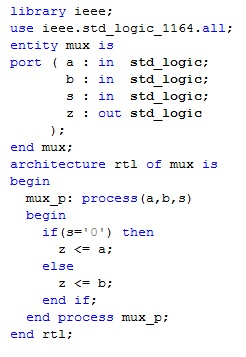
\includegraphics[scale=0.7]{variable_names_before.jpg}
    \caption{}
  \end{subfigure}
  \begin{subfigure}[b]{0.45\textwidth}
    \centering
    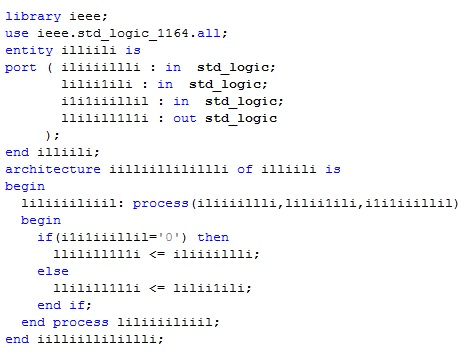
\includegraphics[scale=0.7]{variable_names_after.jpg}
    \caption{}
  \end{subfigure}
  \caption{ а "--- проектное описание до обфускации;
            б "--- после обфускации.}
  \label{fig:fire_alarms}
\end{figure}

\item встраиваемые функции. Часть кода выносится в отдельную функцию, а сам код заменяется вызовом этой функции. Результат синтеза остаётся тем же, злоумышленнику сложнее отследить потоки данных в исходном коде программы.


\begin{figure}[ht]
\centering
  \begin{subfigure}[b]{0.45\textwidth}
    \centering
    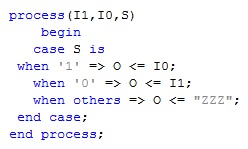
\includegraphics[scale=0.7]{inlining_before.jpg}
    \caption{}
  \end{subfigure}
  \begin{subfigure}[b]{0.45\textwidth}
    \centering
    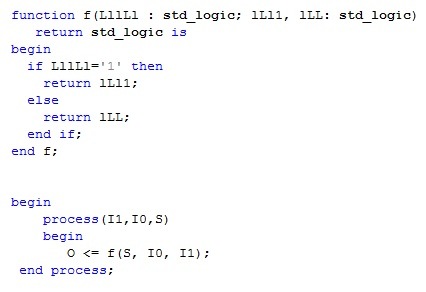
\includegraphics[scale=0.7]{inlining_after.jpg}
    \caption{}
  \end{subfigure}
  \caption{ а "--- проектное описание до обфускации;
            б "--- после обфускации.}
  \label{fig:fire_alarms}
\end{figure}

\item фиктивные выражения(bogus statements). В код добавляются выражения, не несущие никакого  логического смысла, однако затрудняют понимание кода злоумышленником.


\begin{figure}[ht]
\centering
  \begin{subfigure}[b]{0.45\textwidth}
    \centering
    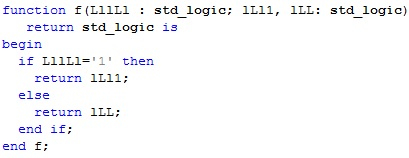
\includegraphics[scale=0.65]{bogus_before.jpg}
    \caption{}
  \end{subfigure}
  \begin{subfigure}[b]{0.45\textwidth}
    \centering
    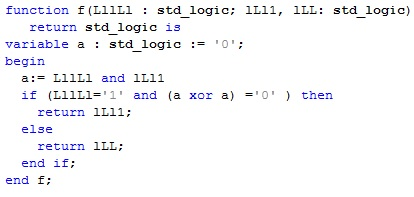
\includegraphics[scale=0.7]{bogus_after.jpg}
    \caption{}
  \end{subfigure}
  \caption{ а "--- проектное описание до обфускации;
            б "--- после обфускации.}
  \label{fig:fire_alarms}
\end{figure}


\item дублирование кода. В код вставляются одинаковые по логике, однако внешне разные по виду фрагменты кода. Позволяет усложнить понимание кода злоумышленником.


\begin{figure}[ht]
\centering
  \begin{subfigure}[b]{0.45\textwidth}
    \centering
    
\includegraphics[scale=0.7]{dup_before.jpg}
    \caption{}
  \end{subfigure}
  \begin{subfigure}[b]{0.45\textwidth}
    \centering
    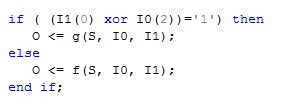
\includegraphics[scale=0.7]{dup_after.jpg}
    \caption{}
  \end{subfigure}
  \caption{ а "--- проектное описание до обфускации;
            б "--- после обфускации.}
  \label{fig:fire_alarms}
\end{figure}

\end{itemize}

Также существуют другие типы лексических преобразований:
\begin{itemize}
\item добавление нового уровня интерпретации. Определяется собственный набор инструкций, программа переводится на новый набор инструкций, пишется интерпретатор для данного набора инструкций. Как результат, программа станровится в 10-100 раз медленнее.
\item chengxification. Представляет собой разворачивание потока управления программы. Каждый оператор помещается внутрь условной конструкции switch и выполняется при определенном условии.
\item array aliasing. Создаётся массив со значениями, в котором каждый элемент определенной периодичности имеет значение, подчиняющееся какой-то логике\cite{collberg}:
    \subitem каждая третья ячейка(розового цвета, см. рисунок ниже), начиная с первой(нулевой), имеет значение 1 mod 5
    \subitem ячейки 2 и 5(зеленого цвета, см. рисунок ниже) содержат значения 1 и 5 соответственно
    \subitem каждая третяя ячейка(голубого цвета, см. рисунок ниже), начиная со второй(первой), имеет значение 2 mod 7
    \subitem ячейки 8 и 11(желтого цвета, см. рисунок ниже) содержат значения 2 и 7 соответственно.

\begin{figure}[ht]
\centering
  \begin{subfigure}[b]{1\textwidth}
    \centering
    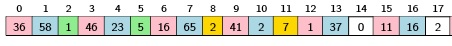
\includegraphics[scale=0.7]{array_aliasing.jpg}
    \caption{}
  \end{subfigure}
  \caption{ графическое представление массива }
  \label{fig:fire_alarms}
\end{figure}

Однако, в силу специфики языка, эти методы плохо применимы(или неприменимы вовсе) к VHDL.
\end{itemize}

\subsubsection{Функциональная обфускация}~\\


Функциональность устройства $Sch$ можно определить как зависимость значений на выходных портах $OP$ от значений на входных портах $IP$, внутренних блоков $B$ и проводящих линий $L$ \cite{ivaniuk}:

\begin{equation}
  OP = F_{Sch} (IP;B;L) \text{\,.}
  \label{eq:domain:functional:basis}
\end{equation}

Пусть существует другое устройство $Sch'$, схема которого описывается выражением

\begin{equation}
  Sch' = \{IP;OP;B';L'\} \text{\,,}
  \label{eq:domain:lexical:schema}
\end{equation}
при этом множество блоков $B'$ и множество линий $L'$ не совпадают с аналогичными множествами устройства $Sch$.

Устройства $Sch$ и $Sch'$ будут функционально эквивалентными, если выполняется следующее равенство\cite{ivaniuk}:
\begin{equation}
  F_{Sch}(IP;B;L) = F_{Sch'}(IP;B';L') \text{\,.}
  \label{eq:domain:functional:basis}
\end{equation}

Функционально эквивалентное преобразование - это замена одного фрагмента кода $V_1 = \{T;S;D;K\}$, результат синтеза которого
\begin{equation}
  DD(V_1) = DD(\{T;S;D;K\}) = \{IP;OP;B;L\} = S_{ch_1} \text{\,,}
  \label{eq:domain:functional:schema}
\end{equation}
другим фрагментом $V_2 = \{T';S';D';K'\}$, результат синтеза которого
\begin{equation}
  DD(V_2) = DD(\{T';S';D';K'\}) = \{IP;OP;B';L'\} = S_{ch_2} \text{\,.}
  \label{eq:domain:functional:schema}
\end{equation}

При этом $Sch_2$ не совпадает с $Sch_1$. Однако наблюдаемое поведение \cite{collberg} обеих схем идентично.

Тогда преобразование функциональной обфускации - это функциональное эквивалентное преобразование, для которого дополнительно выполняется свойство <<сложность результирующей схемы $Sch_2$ выше, чем сложность исходной $Sch_1$>>:

\begin{equation}
  C_{Sch_1}(IP;OP;B;L) = C_{Sch_2}(IP;OP;B';L') \text{\,.}
  \label{eq:domain:functional:schema}
\end{equation}

\subsubsection{Генераторы константных значений}~\\

Множество функциональных обфусцирующих преобразований основывается на генераторах константных значений. Проблема состоит в том, чтобы избежать упрощения схемы. Ниже приведены примеры реализации генераторов константных значений и результат их синтеза. На основе этих элементов можно производить преобразования базовых вентилей. Примером функциональной обфускации может быть мультиплексор, первый вход которого подключен к константе 0. Такая схема эквивалентна вентилю and. С помощью некоторых ухищрений можно добиться того, что синтезатор не распознает в данной схеме and.


\begin{figure}[ht]
\centering
  \begin{subfigure}[b]{1\textwidth}
    \centering
    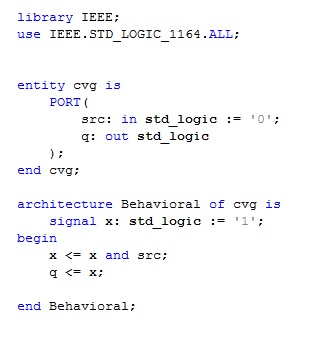
\includegraphics[scale=1]{cvg_code_1.jpg}
    \caption{}
  \end{subfigure}
  \begin{subfigure}[b]{1\textwidth}
    \centering
    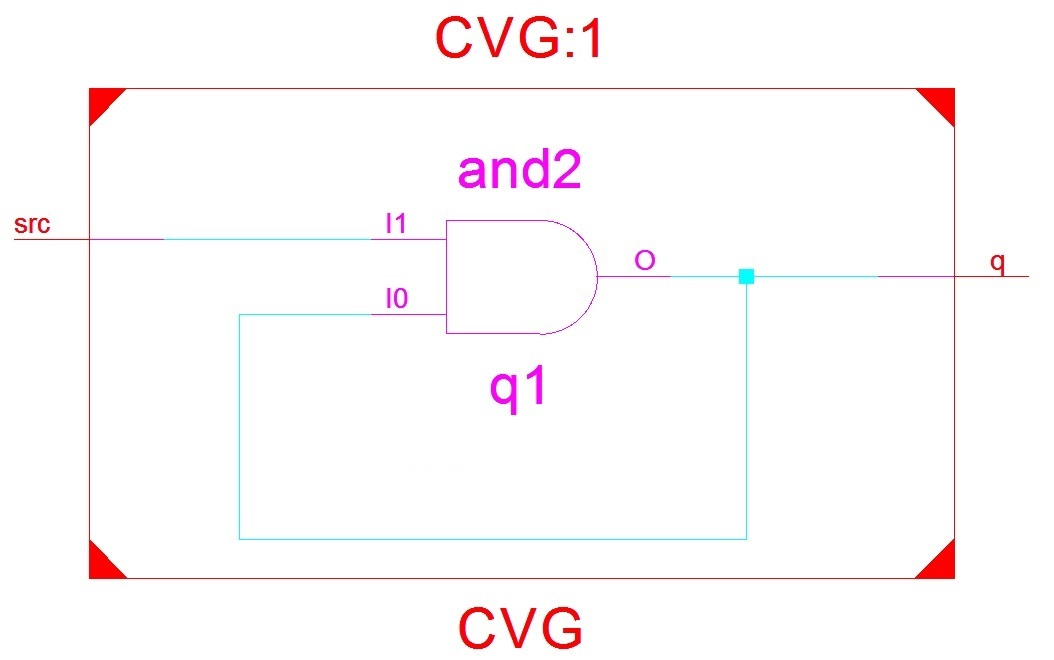
\includegraphics[scale=0.5]{cvg_scheme_inverted_1.jpg}
    \caption{}
  \end{subfigure}
  \caption{ Генератор константных значений с использованием комбинационной логики: а "--- исходный код;
            б "--- результат синтеза.}
  \label{fig:fire_alarms}
\end{figure}



\begin{figure}[ht]
\centering
  \begin{subfigure}[b]{1\textwidth}
    \centering
    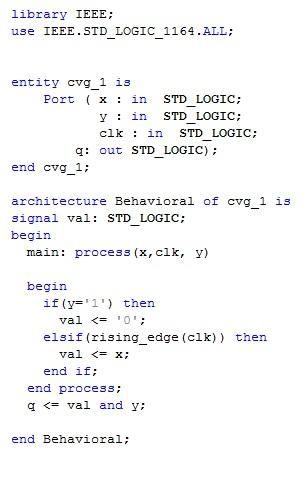
\includegraphics[scale=1]{cvg_code_2.jpg}
    \caption{}
  \end{subfigure}
  \begin{subfigure}[b]{1\textwidth}
    \centering
    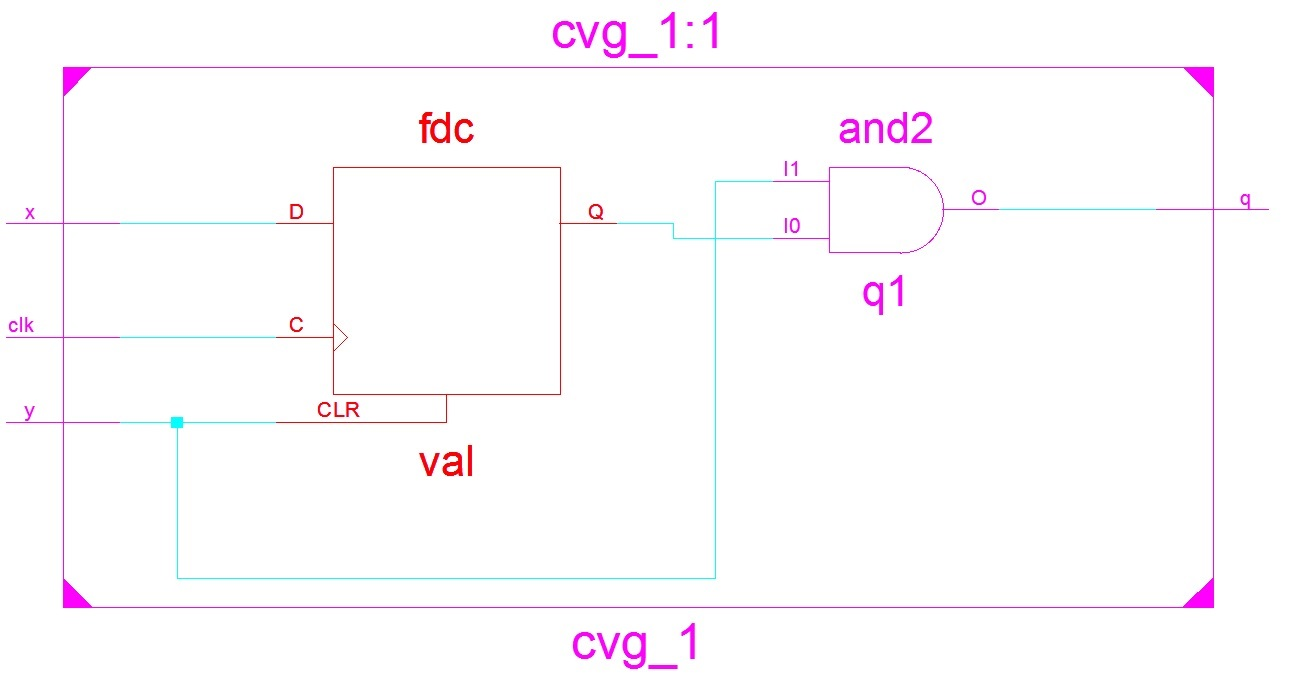
\includegraphics[scale=0.5]{cvg_scheme_inverted_2.jpg}
    \caption{}
  \end{subfigure}
  \caption{ Генератор константных значений с элементом памяти: а "--- исходный код;
            б "--- результат синтеза.}
  \label{fig:fire_alarms}
\end{figure}





\begin{figure}[ht]
\centering
  \begin{subfigure}[p]{1\textwidth}
    \centering
    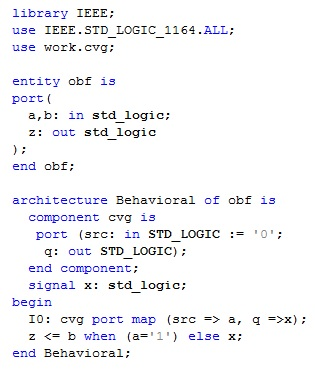
\includegraphics[scale=1]{obfand_code.jpg}
    \caption{}
  \end{subfigure}
  \begin{subfigure}[b]{1\textwidth}
    \centering
    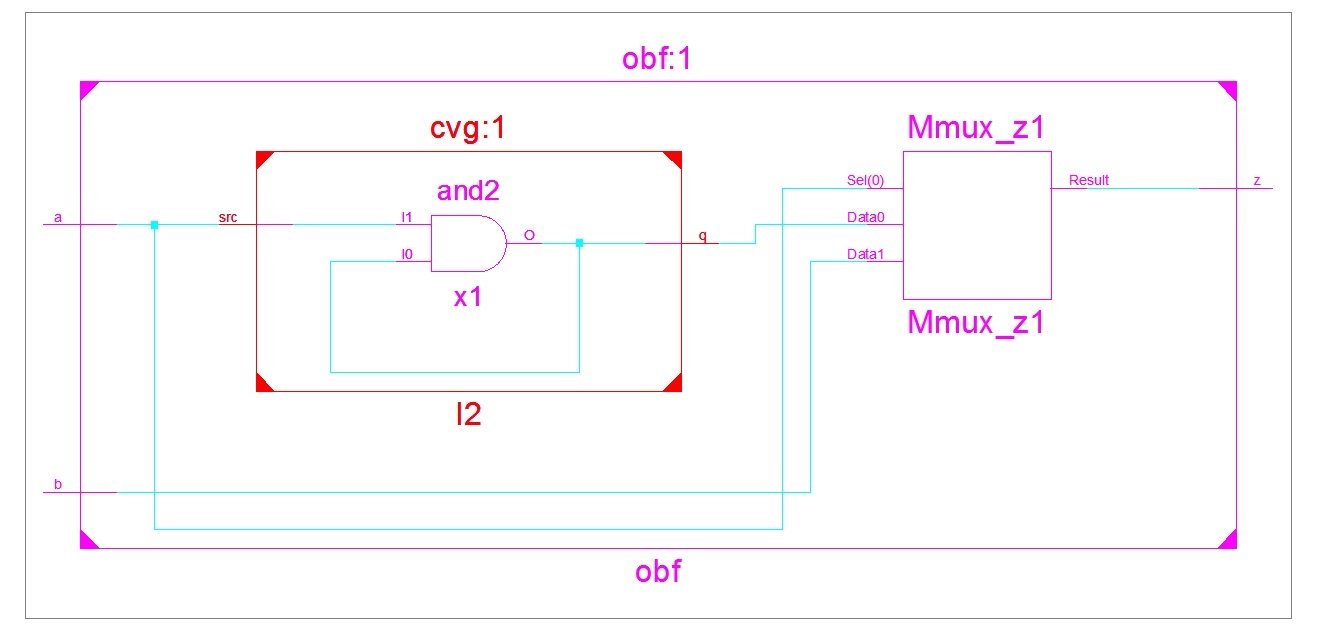
\includegraphics[scale=0.5]{obfand_scheme.jpg}
    \caption{}
  \end{subfigure}
  \caption{ Обфусцированный вентиль and: а "--- исходный код;
            б "--- результат синтеза.}
  \label{fig:fire_alarms}
\end{figure}

\FloatBarrier

\subsection{Обзор существующих аналогов}

Техники и алгоритмы, описанные выше, уже реализованы в программных продуктах фирм xilinx и aldec, однако, поскольку эти продукты являются закрытыми и не могут быть запущены вне этого программного комплекса, то сравнительный анализ данного программного средства с оными невозможен. Исходя из отсутствия свободно распространяемых утилит по обфускации проектных описаний цифровых устройств, разработка данного программного средства имеет смысл.
% \begin{explanation}


\subsection{Постановка задачи}
В результате выполнения дипломного проекта должно быть разработано программное средство лексической и функциональной обфускации проектных описаний цифровых устройств, описанных на языке VHDL со следующими спецификациями:
\begin{itemize}
\item Разрабатываемое ПО должно иметь возможность запускаться под платформами Windows(7,8,10) и Linux(Ubuntu, Arch Linux, Linux Mint)
\item ПО работает в совокупности с другими средствами описания аппаратуры интегральных схем и должно иметь возможность запускаться в форме скрипта.
\item Разрабатываемое ПО должно позволять производить только лексическую(или только функциональную) обфускацию в зависимости от требований конечного пользователя.
\item Время работы ПО должно быть приемлемым.
\end{itemize}
%   где $IP$ "--- множество входных портов; $OP$ "--- множество выходных портов;\\$B$ "--- множество функциональных блоков, из которых состоит схема\\ устройства; $L$ "--- множество проводящих линий, соединяющих внутренние\\ блоки и порты.
% \end{explanation}


% Байесовы сети являются разновидностью вероятностных графовых моделей (Probabilistic Graphical Models, PGM), представляющих вероятностные и причинно"=следственные отношения между переменными в статистическом информационном моделировании~\cite{terehov_2003}.
% Вероятностные сети являются одним из возможных способов представления совместного распределения множества случайных величин.
% Данный способ представления распределения является более компактным, чем хранение вероятностей для всех возможных назначений.
% Здесь и далее под назначением случайных величин $ X_1, X_2, \dotsc, X_n $ понимаются определенные значения, которые принимают случайные величины, т.\,е. значения $ x_1, x_2, \dotsc, x_n $.
% Табличное представление совместного распределения растет экспоненциально количеству переменных и состояний, которые эти переменные могут принимать.
% Например, чтобы задать совместное распределение $ 100 $ бинарных случайных величин необходимо запомнить $ 2^{100} - 1 $ параметр распределения, что не представляется возможным.
% Помимо компактного представления функции распределения такие сети кодируют отношения безусловной и условной независимости, что является важным для понимания причинно"=следственных отношений между переменными в решаемой задаче.
% Благодаря информации о независимости, распределение $ P(X_1, X_2,\dotsc, X_n) $ может быть факторизовано более просто, чем с использованием правила разложения условных вероятностей $ P(X_1, X_2,\dotsc, X_n) = P(X_1) P(X_2|X_1) \dotsm P(X_n|X_1,\dotsc,X_{n-1}) $.
% Если имеется некая классическая байесова сеть, значит она кодирует информацию о независимости между переменными.
% При наличии данной информации совместное распределение случайных величин может быть факторизовано по формуле:
% \begin{equation}
%   \label{eq:domain:bayes_net:joint_disitr}
%   P(X_1, X_2,\dotsc, X_n) = \prod_{i = 0}^{n}{P(X_i|X_{\pi_i})} \text{\,,}
% \end{equation}
% \begin{explanation}
% где & $ \pi_i $ & множество индексов переменных"=родителей для переменной $X_i$.
% \end{explanation}

% Данное представление совместного распределения все так же имеет экспоненциальный рост количества стохастических параметров от количества переменных и их состояний.
% Но на практике, обычно сети имеют небольшую связанность, далекую от полного графа, что позволяет представлять совместное распределение с помощью достижимого количества параметров.


% \label{page:domain:bayes_mod}
% Необходимо отметить, что существует пример успешного коммерческого применения одной из модификаций классической байесовой сети, которая имеет полиномиальный порядок роста количества параметров.
% К сожалению, работы, в которых данные сети были бы формализованы и математически доказана их корректность, пока не публиковались в открытых источниках.
% Отличие данной модификации от классических байесовых сетей заключается в том, что таблицы условных распределений $ P(X_k | X_{\pi_k}) $, где $k$ "--- индекс случайной величины, ассоциированные с вершинами графа и имеющими размерность $ \alpha_k \cdot \prod_{j \in \pi_k}\alpha_j $, заменяются на $ n $ таблиц меньшего размера, представляющих условные распределения $ P(X_k | X_j) $, где $ j \in \pi_k,\ k = 1,\dotsc,n $, ассоциированных с дугами графа и имеющими общую размерность $ \alpha_k \cdot \sum_{j \in \pi_k}\alpha_j $, где $\alpha_j$~--- количество значений, которые может принимать случайная величина $X_j$.
% Также в данной модификации вершины графа содержат таблицы безусловного распределения $ P(X_k) $.
% В связи с указанными изменениями в данной модификации используются несколько другие алгоритмы вывода статистических суждений.
% Разработанная в рамках дипломного проекта библиотека кода предназначена для работы именно с такой модификацией байесовых сетей, т.\,к. различных инструментов для работы с классическими байесовыми сетями создано достаточно.
% Несмотря на это, было сделано предположение, что структура классической байесовой сети и описанной выше модификации будет совпадать, и алгоритмы построения, применимые для нахождения структуры по данным для классической байесовой сети, подойдут для указанной модификации.
% Следовательно, сама библиотека может быть использована и для вывода структуры классических сетей, что будет неоднократно использовано далее для оценки качества структуры сети, полученной по экспериментальным данным.

% Таким образом можно выделить следующие понятия и компоненты, из которых состоят вероятностные сети~\cite{terehov_2003}:
% \begin{itemize}
%   \item множество случайных переменных и направленных связей между переменными;
%   \item каждая переменная может принимать одно из конечного множества взаимоисключающих значений;
%   \item переменные вместе со связями образуют ориентированный граф без циклов;
%   \item каждой переменной"=потомку $X_k$ с переменными"=предками $\pi_k$
% приписывается таблица условных вероятностей $P(X_k | X_{\pi_k})$, либо, для вышеупомянутой модификации "--- каждой дуге между переменными $ X $ и $ Y $ сопоставляется таблица условного распределения $ P (X | Y)$, каждой вершине "--- таблица безусловного распределения $ P(X) $.
% \end{itemize}

% %Что такое байесовы сети (2 стр)

% \subsection{Построение вероятностной сети}
% \label{sub:domain:learning_structure}
% Одним из первых этапов применения байесовых сетей для решения практической задачи, после формулирования проблемы в терминах вероятностей и выделения целевых переменных, является этап описания отношений <<причина"=следствие>> между переменными в виде ориентированных ребер графа~\cite{terehov_2003}.
% Задание подобных отношений определяет структуру графа вероятностной сети.

% От правильности выбора структуры сети зависят многие важные качественные показатели сети, такие как количество необходимых параметров, сложность вывода статистических суждений, возможность обоснования поведения сети при изменении назначений некоторых из переменных.

% Исторически одним из первых способов создания байесовых сетей было привлечение экспертов в предметной области решаемой проблемы.
% Построенная сеть отражала субъективное представление экспертов о проблеме и потенциально могла отличаться от истины.
% Параметры условных распределений в вершинах графа отражали байесовы вероятности по мнению экспертов.
% Здесь и далее под байесовой вероятностью понимается степень уверенности в истинности суждения определенного индивидуума, в отличие от частотной вероятности, которая определяется как относительная частота возникновения события в большом числе испытаний.

% Далее будет рассмотрен пример ручного построения классической байесовой сети по имеющимся априорным данным о проблеме.

% %О важности вывода структуры (1 стр)

% \subsection{<<Ручное>> построение структуры на основе экспертных знаний}
% \label{sub:domain:manual_structure}
% Рассматриваемый здесь пример был взят из домашнего задания, предлагаемого в онлайн курсе Стэндфордского университета по вероятностным графовым моделям~\cite{pgm_course}.
% Ниже приводится один из возможных вариантов его решения.

% Необходимо разработать модель для  прогнозирования своевременности выплат клиентом задолженности банку по кредиту и другим займовым операциям, т.\,е. модель для оценки кредитоспособности клиента банка.
% Банк имеет доступ к некоторой информации о клиенте, такой как его \emph{доходы} (Income), \emph{история платежей} (PaymentHistory), накопленные \emph{богатства} (Assets), \emph{возраст} клиента (Age), а также к \emph{соотношению долгов к доходам} (DebtIncomeRatio).
% Банковский эксперт полагает, что целевая переменная "--- \emph{кредитоспособность} (CreditWorthiness) "--- в конечном итоге зависит от \emph{надежности} (Reliability) клиента, его прогнозируемых \emph{будущих доходов} (FutureIncome) и \emph{соотношения долгов к доходам}.
% По известным на данный момент данным можно построить скелет будущей вероятностной сети "--- её структуру.
% Для полноты картины создания сети вручную пример продолжается и добавляется дополнительная информация, имеющаяся у банка, которая поможет задать вероятности в таблицах условного распределения.
% Необходимо отметить, что указанные вероятности будут байесовыми, т.\,к. отражают субъективное представление о поведении модели:
% \begin{itemize}
%   \item чем лучше история платежей клиента, тем с большей вероятностью он надежен;
%   \item чем старше клиент, тем с большей вероятностью он надежен;
%   \item у старших клиентов с большей вероятностью будет отличная история платежей;
%   \item клиенты с высоким соотношением долгов к доходам с большей вероятностью имеют финансовые трудности, следовательно с меньшей вероятностью имеют хорошую историю платежей;
%   \item чем выше доход человека, тем больше вероятность что он имеет много накопленных богатств;
%   \item чем больше накопленных богатств и выше доходы клиента, тем лучше прогнозируемые будущие доходы;
%   \item при прочих равных, надежные люди с большей вероятностью кредитоспособны, чем ненадежные. Также люди с более высокими прогнозируемыми доходами или с низким соотношением долгов к доходам более кредитоспособны и наоборот.
% \end{itemize}

% С учетом всех приведенных выше дополнительных наблюдений, имеющихся у банка, можно сконструировать сеть и задать байесовы вероятности в таблицах распределения.
% Одна из возможных структур сети приведена на рисунке~\ref{fig:domain:manual_structure:credit_net}.
% Перевод условных обозначений, используемых на рисунке, на русский язык приведен ранее в тексте данного подраздела.
% Таблицы с условными и безусловными вероятностями здесь не приводятся для экономии места.

% Таким образом, чтобы построить классическую байесову сеть понадобилось ознакомиться с предметной областью и проконсультироваться с экспертом.
% Также необходимо было учесть все наблюдения, сделанные экспертом, и учесть его опыт и представление о предметной области.
% В итоге была построена модель, которая соответствует представлению о проблеме эксперта, но на самом деле может отличаться от истинной модели проблемы.

% \begin{figure}[ht]
% \centering
%   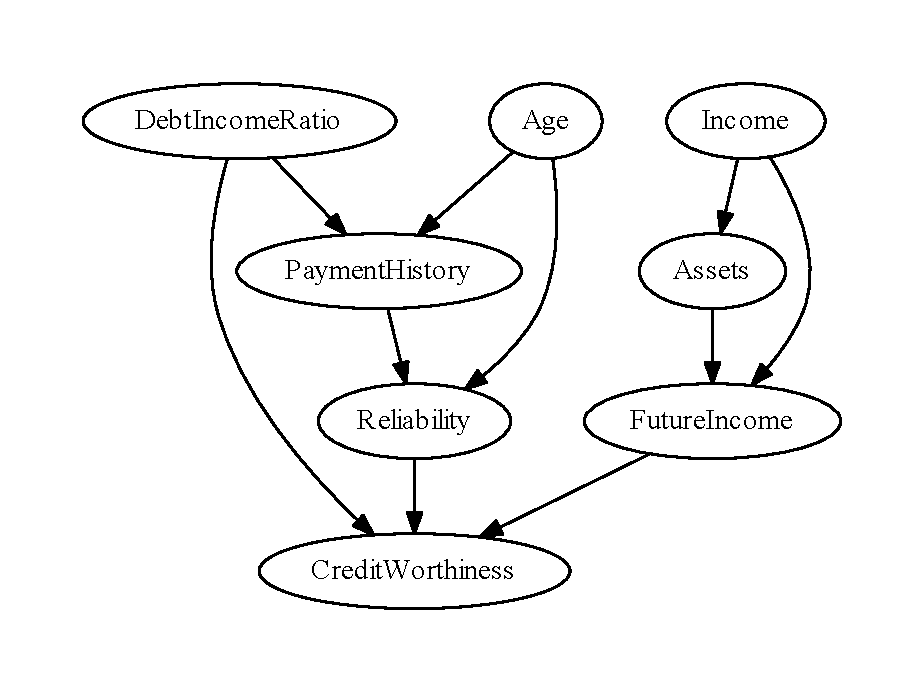
\includegraphics[scale=1]{Credit_net.pdf}
%   \caption{ Байесова сеть для оценки кредитоспособности. }
%   \label{fig:domain:manual_structure:credit_net}
% \end{figure}

% % 2 стр

% \subsection{Сложность нахождения структуры по данным}
% \label{sub:domain:learning_complexity}

% В предыдущем подразделе был приведен пример построения классической байесовой сети <<вручную>> с использованием экспертных знаний.
% Для большинства возникающих задач можно собрать большой объём экспериментальных данных без каких"=либо усилий.
% В данной ситуации возникает интересная задача "--- как построить вероятностную сеть используя лишь эти данные, прибегнув к минимуму экспертных знаний?
% Данный вопрос затрагивался во многих научных работах~\cite{Lam94learningbayesian,Suzuki93,Cooper1991,terentyev_2006} и имеет различные подходы к решению, но сама задача является $\mathcal{NP}$-полной~\cite{Chickering96learningbayesian} и требует применения различных ухищрений и эвристик для автоматического построения структуры сети на практике.

% Сложность задачи обоснована тем, что количество всевозможных назначений растет экспоненциально количеству переменных и их состояний.
% Различные алгоритмы построения сетей используют различные оценочные метрики качества сети.
% Эти метрики, обычно, включают себя подсчёт маргинализованных распределений некоторого подмножества случайных величин.
% Вычисление данных распределений подразумевает подсчет суммы вероятностей экспоненциального числа назначений.
% На практике во избежание большого количества вычислений используются различные приближенные методы, зависящие от метрики.
% Даже при наличии возможности вычислить функцию для оценки качества сети быстро, все равно остаётся проблема супер"=экспоненциального роста количества моделей в зависимости от числа переменных.
% Робинсон в работе~\cite{robinson_1977} предложил следующее рекуррентное соотношение для подсчета числа ацикличных моделей:
% \begin{equation}
%   r (n) =
%   \begin{cases}
%       1 &, n = 0 \\
%       \sum_{i = 1}^{n} (-1)^{i+1} \binom{n}{i} 2^{i(n-i)} r(n - i) &, n > 0
%   \end{cases} % = n ^{2^{\mathcal{O}(n)}}
% \end{equation}

% Для убедительности приведем в таблице~\ref{table:domain:learning:number_of_models} некоторые числа, касающиеся количества возможных моделей для сети из $n$ переменных~\cite{terentyev_2006}.
% Как видно из таблицы, для более семи вершин полный перебор выполнить проблематично.

% \begin{table}[ht]
% \caption{Зависимость числа моделей без циклов от количества вершин, которые нужно проанализировать при полном переборе моделей}
% \label{table:domain:learning:number_of_models}
% \centering
%   \begin{tabular}{| >{\centering}m{0.1\textwidth}
%                   | >{\raggedleft}m{0.345\textwidth}
%                   | >{\centering}m{0.1\textwidth}
%                   | >{\raggedleft\arraybackslash}m{0.345\textwidth}|}
%   \hline Число вершин & \begin{center} Моделей без циклов \end{center} & Число вершин & \begin{center} Моделей без циклов \end{center} \\
%   \hline \num{1} & \num{1} & \num{6} & \num{3781503} \\
%   \hline \num{2} & \num{3} & \num{7} & \num{1138779265} \\
%   \hline \num{3} & \num{25} & \num{8} & \num{783702329343} \\
%   \hline \num{4} & \num{543} & \num{9} & \num{1213442454842881} \\
%   \hline \num{5} & \num{29281} & \num{10} & \num{4175098976430598100} \\
%   \hline
%   \end{tabular}
% \end{table}

% %Указание что это NP трудная задача (0.5)
% %Табличка с оценкой количества сетей в зависимости от числа переменных (для устрашения) (0.2)

% \subsection{Принцип минимальной длинны описания}
% \label{sub:domain:mdl_principle}
% В данном подразделе рассматривается принцип минимальной длинны описания\footnote{В англоязычной литературе используется термин minimum description length или сокращенно MDL.} (МДО) и его применимость для задания функции оценки качества обучаемой сети.
% Данный принцип позволяет среди множества моделей выбрать модель с оптимальным соотношением сложности и соответствием модели наблюдаемым данным.
% Т.\,е. данный принцип позволяет выбрать несложную и <<полезную>> модель, устойчивую к проблеме переобучения\footnote{В англоязычной литературе данная проблема называется overfitting и подразумевает, что модель слишком хорошо объясняет данные на которых она обучалась, но из-за этого непригодна для прогнозирования "--- работе на данных ранее не известных.}.
% Принцип МДО в своей нестрогой и наиболее общей формулировке гласит: среди множества моделей следует выбрать ту, которая позволяет описать данные наиболее коротко, без потери информации~\cite{Grunwald05atutorial}.
% В контексте поиска модели байесовой сети, соответствующей экспериментальным данным, принцип МДО гласит, что нужно выбрать модель, которая минимизирует сумму длин кодирования самой модели и кодирования экспериментальных данных с помощью этой модели~\cite{Lam94learningbayesian}, что выражается формулой:
% \begin{equation}
%   \label{eq:domain:mdl:description_length}
%   l(x^{R}[n]) = \min_{g \in G}\left[ l_{G}(g) + l_{g}(x^{R}[n]) \right] \text{\,,}
% \end{equation}
% \begin{explanation}
% где & $ x^R $ & вектор размерностью $R$, содержащий значения переменных (аттрибутов). Представлен как $ x^R =\newline= (x^{(1)}, x^{(2)}, \dotsc, x^{(R)} ) $, где атрибут $ x^{(j)} $ может принимать $ \alpha_{j} $ значений, $ j = 1,\dotsc,R.$ \\
%     & $ n $ & количество случаев в экспериментальных данных;  \\
%     & $ x^R[n] $ & набор экспериментальны данных; \\
%     & $ G $ & множество моделей; \\
%     & $ l_{G}(g) $ & длина описания модели; \\
%     & $ l_{g}(x^{R}[n]) $ & длина представления данных $ x^R[n] $ моделью $ g \in G $.
% \end{explanation}

% Для вычисления длинны кодирования модели и длинны кодирования данных с использованием модели в реализации дипломного проекта использовались результаты, приведенные в работах~\cite{Suzuki93,terentyev_2006}.
% Собственно модель вероятностной сети состоит из таблиц условных и безусловных распределений и отношений <<родитель"=потомок>> между вершинами.
% Для вычисления длины кодирования модели можно воспользоваться формулой~(\ref{eq:domain:mdl:model_length}):
% \begin{equation}
%   \label{eq:domain:mdl:model_length}
%   l_{G}(g) = \frac{\log{n}}{2} \cdot \sum_{k = 1}^{R} S_k(g) (\alpha_k - 1) \text{\,,}
% \end{equation}
% \begin{explanation}
% где & $ S_k(g) $ & количество возможных назначений переменных"=родителей переменной $X_k$, способ вычисления данного значения отличается у классических сетей и модификации упомянутой в разделе~\ref{sub:domain:bayes_net} на странице~\pageref{page:domain:bayes_mod}.
% \end{explanation}

% Значение функции $S_k(g)$ для классических байесовых сетей вычисляется по формуле~(\ref{eq:domain:mdl:classic_parent_states}), для модификации упомянутой в разделе~\ref{sub:domain:bayes_net} на странице~\pageref{page:domain:bayes_mod} "--- по формуле~(\ref{eq:domain:mdl:mod_parent_states}):
% \begin{align}
%   \label{eq:domain:mdl:classic_parent_states}
%   S_k(g) &= \prod_{j \in \pi_k}\alpha_j \text{\,,} \\
%   \label{eq:domain:mdl:mod_parent_states}
%   S_k(g) &= \sum_{j \in \pi_k}\alpha_j \text{\,.}
% \end{align}

% Длинна представления данных $ l_{g}(x^{R}[n]) $ вычисляется как эмпирическая энтропия $ n $ экспериментальных наблюдений $ x^{R}[n] $ при заданной модели $ g $.
% Эмпирическая энтропия может быть вычислена по формуле~(\ref{eq:domain:mdl:data_entrophy}):
% \begin{equation}
%   \label{eq:domain:mdl:data_entrophy}
%   \mathcal{H}(x^{R}[n] | g) =
%     \sum_{k = 1}^{R}
%     \sum_{s = 1}^{S_{k}(g)}
%     \sum_{q = 0}^{\alpha_{k + 1} - 1}
%     -n[q, s, k, g] \log \frac{n[q, s, k, g]}{n[s, k, g]} \text{\,,}
% \end{equation}
% \begin{explanation}
% где & $ n[s, k, g] $ & количество случаев в экспериментальных данных $ x^R[n] $ в которых переменные"=родители переменной $X_k$ принимают назначение $s$; \\
%     & $ n[q, s, k, g] $ & количество случаев в экспериментальных данных $ x^R[n] $ в которых переменные"=родители переменной $X_k$ принимают назначение $s$, а переменная $X_k$ принимает назначение $q$.
% \end{explanation}

% Таким образом, приведенные выше формулы, могут быть использованы для оценки качества структуры сети и её сложности.
% Имея данную оценку можно использовать различные стратегии поиска в пространстве возможных моделей, минимизируя целевую функцию~(\ref{eq:domain:mdl:description_length}).
% Более подробно об используемых стратегиях поиска говорится в разделе~\ref{sec:arch_and_mod}.
% За доказательствами и более подробными сведениями о применении принципа МДО в построении байесовых сетей можно обратиться к работам~\cite{Lam94learningbayesian,Suzuki93,terentyev_2006,Grunwald05atutorial}.

% % MDL (2-3)


% \subsection{Оценка структуры сети на основе апостериорной вероятности}
% \label{sub:domain:k2_algo}
% Существуют подходы, использующие байесов метод для оценки качества полученной структуры и алгоритмы на их базе пытаются максимизировать апостериорную вероятность структуры для данного набора экспериментальны данных.
% Один из возможных подходов к оценке качества двух структур приведет в работе~\cite{Cooper1991}.
% В программном обеспечении, разработанном в данном дипломном проекте, использовался критерий оценки качества структуры, приведенный в упомянутой выше работе.

% Введем некоторые обозначения, в дополнение к тем, которые были введены в подразделе~\ref{sub:domain:mdl_principle}.
% Пусть структура вероятностной сети обозначается символом $B_S$, таблицы условных распределений, ассоциированные с сетью, "--- $B_P$.
% Две вероятностные сети для данного набора экспериментальных данных можно оценить по отношению~(\ref{eq:domain:k2:nets_ratio}) апостериорных вероятностей:
% \begin{equation}
%   \label{eq:domain:k2:nets_ratio}
%   \frac{P(B_{S_i} | x^R[n])}{P(B_{S_j} | x^R[n])} =
%     \frac{ \frac{P(B_{S_i}, x^R[n])}{P(x^R[n])} }
%          { \frac{P(B_{S_j}, x^R[n])}{P(x^R[n])} } =
%     \frac{ P(B_{S_i}, x^R[n]) }
%          { P(B_{S_j}, x^R[n]) } \text{\,.}
% \end{equation}

% Как видно из приведенной формулы~(\ref{eq:domain:k2:nets_ratio}), научившись вычислять отношение совместных распределений, можно сравнивать апостериорные вероятности структур.
% Т.\,к. в разработанном ПО использовались результаты, приведенные в работе~\cite{Cooper1991}, то считаем целесообразным привести в данном подразделе базовые формулы и предположения из вышеупомянутой работы.

% Для вычисления $P(B_S, D)$ важно сделать несколько важных предположений:

% \begin{itemize}
%   \item
%   Экспериментальные данные содержат только дискретные случайные величины и все эти случайные величины присутствуют в истинной структуре $B_S$ модели из которой были получены эти экспериментальные данные.
%   Из данного предположения следует формула~(\ref{eq:domain:k2:assumption1}):
%   \begin{equation}
%     \label{eq:domain:k2:assumption1}
%     \int_{B_P} P(x^R[n] | B_S, B_P) f(B_P | B_S) P(B_S) dB_p \text{\,,}
%   \end{equation}
%   \par\hspace{\fivecharsapprox} % абзацный отступ
%   \begin{tabular}{@{}ll@{ --- }p{0.74\textwidth}}
%   где & $ B_P $ & вектор, содержащий значения условных вероятностей для назначений переменных из структуры $ B_S $; \\
%       & $ f $ & условная плотность распределения $B_P$ при условии структуры $B_S$. \\[\parsep]
%   \end{tabular}

%   \item
%   Случаи, зафиксированные в экспериментальных данных, независимы друг от друга, при условии зафиксированной модели, т.\,е. данное предположение подразумевает, что модель, генерирующая экспериментальные данные не меняется.
%   Это предположение позволяет упростить формулу~(\ref{eq:domain:k2:assumption1}) и привести её к виду:
%   \begin{equation}
%     \label{eq:domain:k2:assumption2}
%     P(B_S, x^R[n]) =
%       P(B_S) \int_{B_P} \left[ \prod_{j = 1}^{n} P(x^R_j | B_S, B_P) \right] f(B_P | B_S) dB_P \text{\,.}
%   \end{equation}

%   \item
%   Экспериментальные данные не должны содержать пропущенных значений для переменных из структуры $B_S$.
%   Введем дополнительные обозначения.
%   Пусть $x_j^{(i)}$ представляет значение $i$-й переменной в $j$-м случае.
%   Пусть $\phi_i$ представляет из себя вектор уникальных назначений переменных"=родителей для $i$-й переменной, т.\,е. вектор уникальных назначений для $ \forall X_k,\ k \in \pi_i$.
%   Пусть $\sigma(i, j)$ индексная функция, которая возвращает индекс назначения $\pi_i$ в $j$-ом случае из вектора $\phi_i$.
%   Введем обозначение для длинны вектора $q_i = | \phi_i |$.
%   Теперь с учетом предположения об отсутствии пропущенных значений можно вычислить вероятность конкретного случая из экспериментальных данных по формуле:
%   \begin{equation}
%     \label{eq:domain:k2:case_prob}
%     P(x^R_j | B_S, B_P) =
%       \prod_{i = 1}^{R} = P(X_i = x_j^{(i)} | \phi_i[\sigma(i, j)], B_P) \text{\,.}
%   \end{equation}
%   Подставляя выражение~(\ref{eq:domain:k2:case_prob}) в формулу~(\ref{eq:domain:k2:assumption2}) получим:
%   \begin{align}
%     \label{eq:domain:k2:assumption3}
%     P(B_S, x^R[n]) =
%       P(B_S)
%       \int_{B_P}\left[ \prod_{j = 1}^{n}\prod_{i = 1}^{R} P(X_i = x_j^{(i)} | \phi_i[\sigma(i, j)], B_P)  \right] &\times \notag\\
%       \times f(B_P | B_S) dB_P \text{\,.}
%   \end{align}
%   Пусть для выбранных $i$ и $j$ $f(P(x_i | \phi_i[j], B_P))$ обозначает плотность распределения возможных значений $P(x_i | \phi_i[j], B_P)$.
%   Необходимо сделать еще одно предположение.

%   \item Для $ 1 \le i, i' \le n$, $ 1 \le j \le q_i $, $1 \le j' \le q_i $, если
%   $ij \neq i'j'$, то распределение $f(P(x_i | \phi_i[j]))$ не зависимо от распределения $f(P(x_{i'} | \phi_{i'}[{j'}]))$.
%   Данное предположение по свой сути полагает, что до того, как были получены экспериментальные данные, все возможные назначения равновероятны.
% \end{itemize}

% С учетом приведенных выше предположений и теоремы, приведённой и доказанной в работе~\cite{Cooper1991}, можно привести формулу для вычисления $P(B_S, D)$:
% \begin{equation}
%   \label{eq:domain:k2:model_and_data_prob}
%   P(B_S, x^R[n]) =
%     P(B_S)
%     \prod_{i = 1}^{R}
%     \prod_{j = 1}^{q_i}
%     \frac{(\alpha_i - 1)!}
%          {(n[\phi_i[j], i, B_S] + \alpha_i - 1)!}
%     \prod_{k = 1}^{\alpha_i}
%       n[v_{ik}, \phi_i[j], i, B_S]! \text{\,,}
% \end{equation}
% \par
% \begin{tabular}{@{}ll@{ --- }p{0.74\textwidth}}
% где & $ v_{ik} $ & $k$-е возможное назначение переменной $X_i$. \\[\parsep]
% \end{tabular}

% Формула~(\ref{eq:domain:k2:model_and_data_prob}) позволяет вычислить значение $P(B_S, x^R[n])$, если известна вероятность $P(B_S)$ и подсчитана оставшаяся часть формулы на основе экспериментальны данных $x^R[n]$.
% Но из-за того, что $P(B_S)$ является чаще неизвестной величиной, чем известной, предполагают, что все возможные структуры сети равновероятны и $P(B_S)$ является некой малой константой.
% Апостериорную вероятность структуры, при условии данных можно вычислить по формуле:
% \begin{equation}
%   \label{eq:domain:k2:aposteriori_structure_given_data}
%   P(B_S | x^R[n]) =
%     \frac{P(B_S, x^R[n])}
%          {\sum_{B_S}P(B_S, x^R[n])} \text{\,.}
% \end{equation}

% Но, как уже упоминалось, множество возможных структур слишком велико, и на практике значение апостериорной вероятности можно вычислить лишь для малых сетей либо приблизительно.
% В разделе~\ref{sec:arch_and_mod} будет более подробно рассмотрена модификация оценки апостериорной вероятности~(\ref{eq:domain:k2:model_and_data_prob}), применимая на практике.

% %Оценка апостериорных вероятностей (K2) (2-3)

% \subsection{Общая структура алгоритмов}
% \label{sub:domain:other_algos}
% В предыдущих двух подразделах были рассмотрены два подхода к оценке качества структуры сети при известных экспериментальных данных.
% Как уже упоминалось ранее, выбор функции оценки сети является лишь одним из компонентов большинства алгоритмов построения структуры сети по данным.
% Важной частью алгоритма является также выбор стратегии поиска в пространстве возможных структур.
% От выбора стратегии поиска зависит трудоемкость алгоритма, качество найденной сети и, собственно, её структура.
% В ПО разработанном в рамках дипломного проекта реализовано несколько различных алгоритмов нахождения структуры на основе оценки апостериорной вероятности из подраздела~\ref{sub:domain:k2_algo} и оценки на основе принципа МДО из подраздела~\ref{sub:domain:mdl_principle}.
% Стоит упомянуть, что в разработанном ПО реализованы разные стратегии поиска для разных оценок.
% Так алгоритмы использующие оценку МДО могут находить сети произвольной структуры без каких-либо априорных знаний о предметной области.
% С другой стороны, для уменьшения пространства возможных решений, алгоритм, использующий оценку апостериорной вероятности, требует априорных знаний об упорядоченности переменных.
% В данном конкретном случае, переменные должны быть упорядочены так, что возможные переменные"=родители данной переменной находятся в упорядоченном списке раньше самой переменной.
% Во многих других работах накладываются дополнительные ограничения на структуру выводимой сети.
% Например, в работе~\cite{Suzuki93} используется оценка МДО, но класс находимых структур ограничен деревьями.
% В работе~\cite{Rebane87} приводится алгоритм, ограниченный классом полидеревьев.
% % Ограничения других методов построения (упорядоченность нод, ) (2)

% \subsection{Обзор существующих программ} % (fold)
% \label{sub:domain:existing_programs}
% Cуществует множество решений для работы с классическими байесовыми сетями.
% Ниже приведены некоторые из задач, которые может выполнять типичный редактор вероятностных сетей:
% \begin{itemize}
%   \item ручное, автоматическое, полу"=автоматическое построение структуры сети;
%   \item оценка параметров условных распределений по данным;
%   \item различные алгоритмы статистического вывода суждений в сетях;
%   \item генерация экспериментальных данных по готовой сети;
% \end{itemize}

% Приняв во внимание тему дипломного проекта, наибольший интерес в существуем ПО будет представлять функциональность автоматического вывода структуры сети по данным.
% Ниже рассматриваются некоторые из программ для работы с байесовыми сетями.

% \subsubsection{SAMIAM }(\url{http://reasoning.cs.ucla.edu/samiam})
% Бесплатный кросс"=платформенный редактор байесовых сетей, написанный на Java.
% Имеет богатую функциональность по ручному созданию сетей.
% Поддерживает множество различных алгоритмов вывода статистических суждений и позволяет делать различные типы запросов к сети.
% Позволяет генерировать экспериментальные данные, соответствующие готовой сети.
% Но функциональность, обеспечивающая автоматический вывод структуры сети по данным, отсутствует.

% \subsubsection{Netica }(\url{http://www.norsys.com/netica.html})
% Коммерческое программное обеспечение.
% Версия программы с ограниченной функциональностью свободно доступна на сайте фирмы Norsys.
% Netica "--- мощная, удобная в работе программа для работы с графовыми вероятностными моделями.
% Она имеет интуитивный и приятный интерфейс пользователя для просмотра и редактирования топологии сети.
% Соотношения между переменными могут быть заданы, как индивидуальные вероятности, в форме уравнений, или путем автоматического обучения из файлов данных (которые могут содержать пропуски), но, к сожалению, в бесплатном варианте программы данная функциональность недоступна и возможности сравнить с разработанной в дипломном проекте реализацией нет.
% Созданные сети могут быть использованы независимо, и как фрагменты более крупных моделей, формируя тем самым библиотеку модулей~\cite{terehov_2003}.

% \subsubsection{GeNIe }
% \label{sub:domain:existing_programs:genie}
% (\url{http://genie.sis.pitt.edu/})
% Бесплатное кросс"=платформенное приложение и библиотека для работы с вероятностными графовыми моделями, написанная на \cpp{}.
% Предоставляется функциональность ручного и автоматического создания сетей, а также реализуются алгоритмы вывода статистических суждений.
% Программа реализует несколько алгоритмов вывода структуры сети по данным, целесообразно привести здесь одно небольшое сравнение с разработанным ПО, т.\,к. функциональности приложений пересекаются.
% Более подробное сравнение разработанного ПО с существующим будет произведено в разделе~\ref{sec:arch_and_mod}.
% Уместно рассмотреть хорошо изученную сеть Asia\footnote{\url{http://www.bnlearn.com/bnrepository/\#asia}}.
% Экспериментальные данные, содержащие \num{1000} случаев и имеющие распределение задаваемое сетью, были сгенерированы с помощью одной из вышеперечисленных программ.
% К этим экспериментальным данным были применены три различных алгоритма вывода структуры, реализованные в GeNIe.
% Выведенные структуры приведены на рисунке~\ref{fig:domain:programs:genie_infered_structrures}.
% Для сравнения, структуры, выведенные одним из алгоритмов из разработанной библиотеки на том же наборе данных, и истинная сеть Asia приведены на рисунке~\ref{fig:domain:programs:our_impl_plus_asia}.
% Как видно, алгоритм из разработанной библиотеки не нашел одну связь, в отличие от алгоритмов реализованных в GeNIe, которые допустили больше ошибок в структуре.

% \begin{figure}[ht]
% \centering
%   \begin{subfigure}[b]{0.51\textwidth}
%     \centering
%     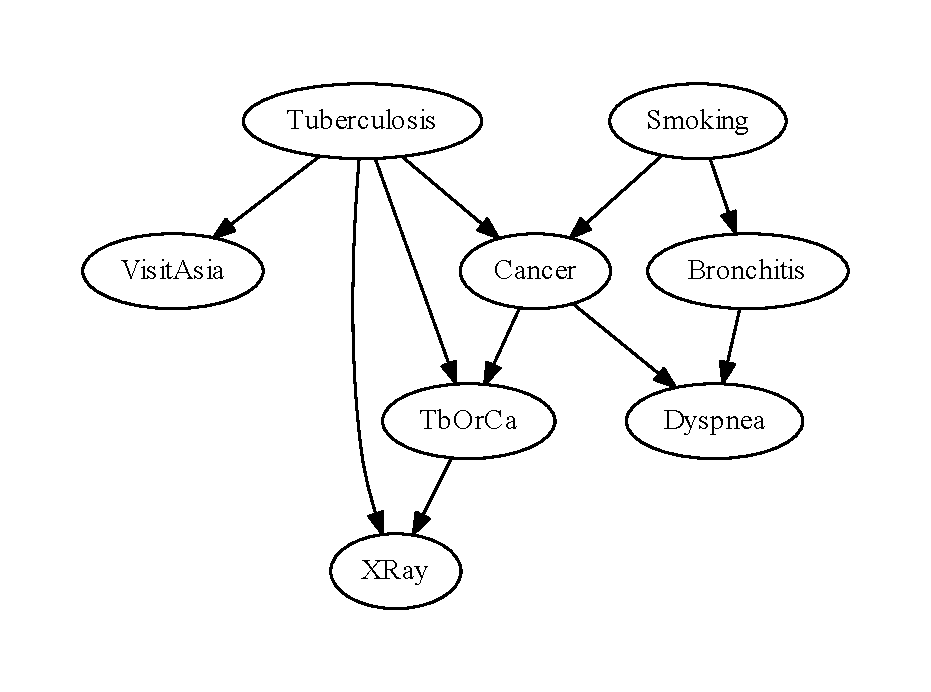
\includegraphics[scale=0.5]{asia_genie_1000_bayesian_search.pdf}
%     \caption{}
%   \end{subfigure}
%   \begin{subfigure}[b]{0.48\textwidth}
%     \centering
%     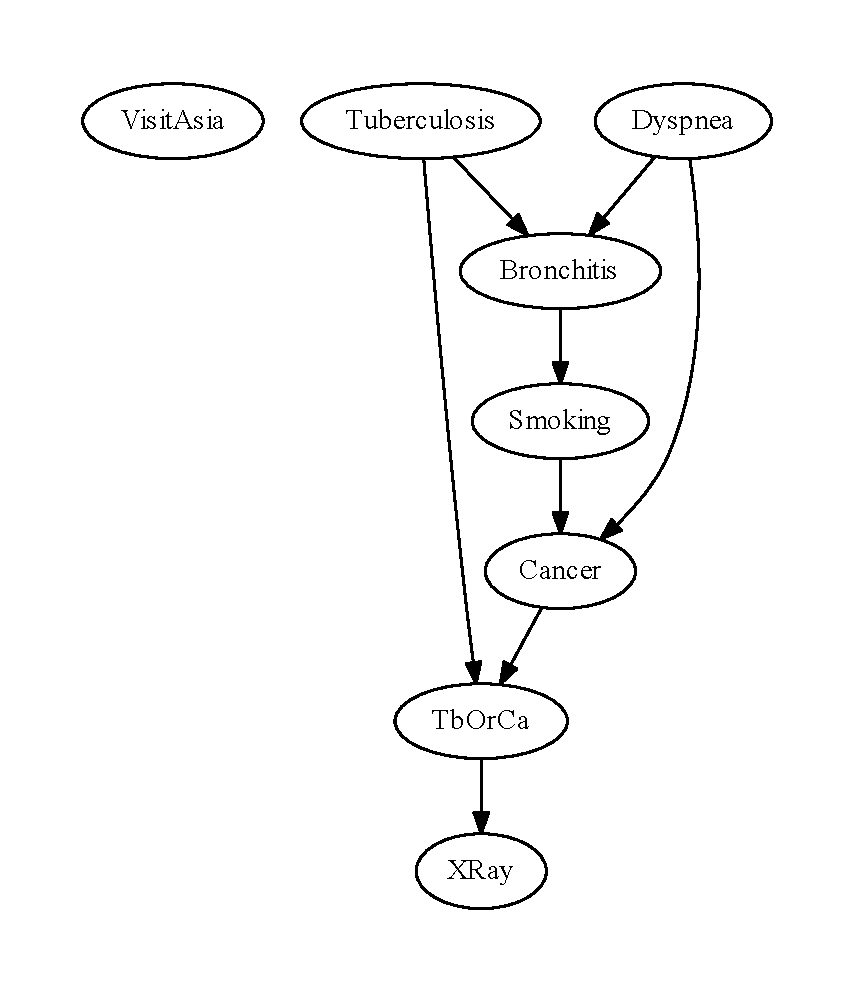
\includegraphics[scale=0.5]{asia_genie_1000_k2.pdf}
%     \caption{}
%   \end{subfigure}
%   \begin{subfigure}[b]{0.9\textwidth}
%     \centering
%     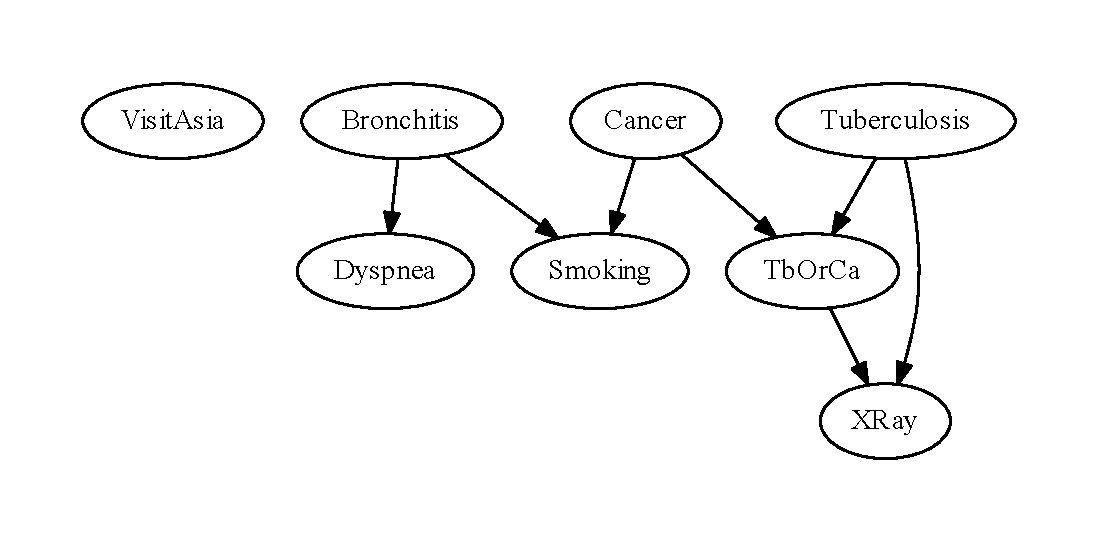
\includegraphics[scale=0.5]{asia_genie_1000_pc.pdf}
%     \caption{}
%   \end{subfigure}
%   \caption{ Структуры, выведенные по данным с помощью GeNIe: а "--- алгоритм Bayesian Search;
%             б "--- алгоритм K2;
%             в "--- алгоритм PC;}
%   \label{fig:domain:programs:genie_infered_structrures}
% \end{figure}


% \begin{figure}[ht]
% \centering
%   \begin{subfigure}[b]{0.49\textwidth}
%     \centering
%     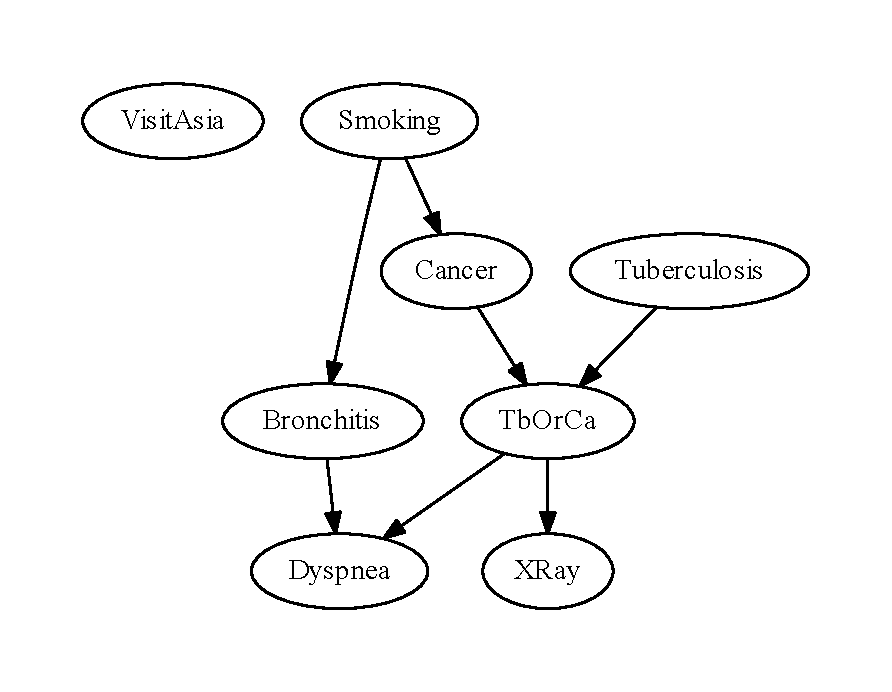
\includegraphics[scale=0.45]{asia-learned-by-terent-random-1000.pdf}
%     \caption{}
%   \end{subfigure}
%   \begin{subfigure}[b]{0.48\textwidth}
%     \centering
%     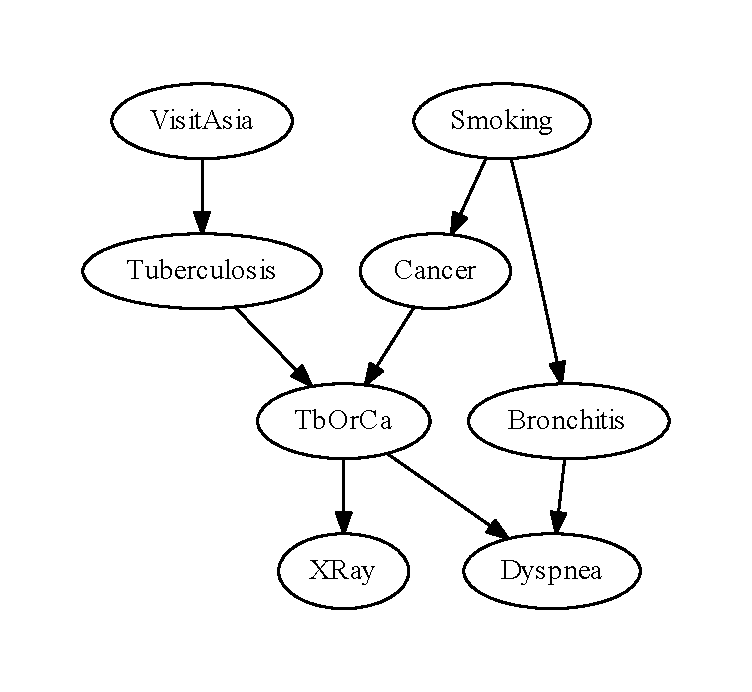
\includegraphics[scale=0.45]{asia_reference_net.pdf}
%     \caption{}
%   \end{subfigure}

%   \caption{ Выведенная из данных и оригинальная сеть Asia: а "--- алгоритм из разработанной библиотеки, использующий оценку МДО;
%             б "--- истинная сеть Asia}
%   \label{fig:domain:programs:our_impl_plus_asia}
% \end{figure}

\lstset{style=fsharpstyle}

\section{Используемые технологии}
\label{sec:practice:technology_used}

Выбор технологий является важным предварительным этапом разработки сложных информационных систем.
Платформа и язык программирования, на котором будет реализована система, заслуживает большого внимания, так как исследования показали, что выбор языка программирования влияет на производительность труда программистов и качество создаваемого ими кода.

Ниже перечислены некоторые факторы, повлиявшие на выбор технологий:
\begin{itemize}
\item разрабатываемое ПО должно иметь возможность запускаться под платформами Windows(7,8,10) и Linux(Ubuntu, Arch Linux, Linux Mint);
\item ПО работает в совокупности с другими средствами описания аппарутры интегральных схем и должно иметь возможность запускаться в форме скрипта;
\item среди различных платформ разработки имеющийся программист лучше всего знаком с разработкой на платформе;
\item дальнейшей поддержкой проекта, возможно, будут заниматься разработчики, не принимавшие участие в выпуске первой версии;
\item имеющийся разработчик имеет опыт работы с объекто-ориентированными языками программирования;
\end{itemize}

Основываясь на опыте работы имеющихся программистов разрабатывать ПО целесообразно с помощью языка Ruby.
Приняв во внимание необходимость обеспечения доступности дальнейшей поддержки ПО, возможно, другой командой программистов, необходимость работы с различными ОС, скриптообразный характер ПО, целесообразно не использовать малоизвестные и сложные языки программирования.
С учетом этого фактора выбор языков программирования сужается до четырех: Perl, Python, Ruby и Lua.
Слабые по сравнению с другими языками механизмы ООП (отсутствие наследования, классов) языка LUA, которые могут быть полезны при разработке ПО, позволяют исключить этот язык из списка кандидатов.
Per уступает по удобству использования двум другим кандидатам из нашего списка.
Оставшиеся два языка программирования Ruby и Python являются первостепенным, мультипарадигменными языками программирования. Однако наличие синтаксического анализатора языка VHDL делает
Ruby предпочтительным кандидатом.
Таким образом, с учетом вышеперечисленных факторов, целесообразно остановить выбор на следующих технологиях:
\begin{itemize}
  \item операционные системы: семейство Windows(7,8,10), семейство Linux(Ubuntu, Debian, Arch Linux), Mac os;
  \item язык описания аппаратуры интегральных схем VHDL;
  \item язык программирования Ruby;
\end{itemize}
Для реализации поставленной задачи предпочительно использовать библиотеку синтаксического анализа языка HDL, помимо этого достаточно использовать стандартные библиотеки указанного выше языка.
Высокий уровень абстракции языка, полноценные механизмы ООП, динамическая система типов позволяют наиболее просто и <<красиво>> позволяет решить возникающую задачу.
Разрабатываемое программное обеспечение в некоторой степени использует данное преимущество языка.
Язык ruby будет использован для создания высокоуровнего дизайна проложения (иерархия классов и интерфейсов, организация модулей и публичного программного интерфейса), реализации логики приложения, функций и методов~\cite{dpir_2007}, прототипирования различных идей.
В разрабатываемом программном продукте Ruby используется для cинтаксического анализа, обработки полученной информации, трансформации исходного кода языка VHDL.


\subsection{Язык программирования Ruby}
\label{sub:practice:ruby_overview}
Ruby -- объектно-ориентированный, динамический язык программирования общего назначения~\cite{ruby_site}.
Язык разрабатывался с целью сделать <<настоящий объектно-ориентированный>>, лёгкий в разработке, интерпретируемый язык программирования.
Для достижения этой цели в языке гармонично сочетаются простота, выразительность.
Создателем языка с первой версии является  Юкихиро Мацумото (Matz).
Язык ruby является платформенно нейтральным, но создавался для хорошей работы с unix-подобными системами.
Этот язык сочетает простой синтаксис, похожий на синтаксис языков Perl и Python, и полную поддержку всех современных объектно-ориентированных концепций и подходов. В качестве ориентира при разработке языка была выбрана динамичность, нацеленная на написание простого и продуктивного кода~\cite{trpr_2011_ru}.

Язык имеет богатую поддержку парадигмы объекто-ориентированного программирования, включающую поддержку инкапсуляции, наследования и полиморфизма.
Отличительными чертами Ruby с точки зрения ОО парадигмы являются:
\begin{itemize}
  \item Динамическая система типов.
        В ruby реализована неявная(утиная) типизация: границы использования объекта определяются его текущим набором методов и свойств, в противоположность наследованию от определённого класса. Это значит, что объект реализует интерфейс, если он содержит все методы этого интерфейса, независимо от связей в иерархии наследования и принадлежности к какому-либо конкретному классу.
        В ruby все типы являются объектами, унаследованными от класса Object.
  \item Классы и интерфейсы.
        В классической объекто-ориентированной парадигме существуют только классы.
        В ruby дополнительно существуют и другие типы, например, модули.
        Модули в ruby похожи на классы в том, что они содержат набор методов, константы, другие модули и определения классов.
        Есть два предназначения модулей. Во-первых, они служат централизованного хранения констант и методов:
        \begin{lstlisting}[language=Ruby, style=rubystyle]
  module Trig
    PI = 3.1416
    # class methods
    def Trig.sin(x)
      # ...
    end
    def Trig.cos(x)
      # ...
    end
  end
        \end{lstlisting}

        Во-вторых, модули позволяют делить функциональность между классами, при включении (include) модуля в класс, его методы добавляются в класс. Такой способ называется примесью (mixin):

        \begin{lstlisting}[language=Ruby, style=rubystyle]
  module MyModule
    GOODMOOD = "happy"
    BADMOOD = "grumpy"

    def greet
      return "I'm #{GOODMOOD}. How are you?"
    end

    def MyModule.greet
      return "I'm #{BADMOOD}. How are you?"
    end
  end

  class MyClass
     include MyModule

    def sayHi
      puts( greet )
    end
  end

  ob = MyClass.new
  ob.sayHi
  puts(ob.greet)
        \end{lstlisting}
        <<Примеси>> могут быть использованы при необходимости проведения множественного наследования (в отличие от языков \cpp{} и Eiffel, ruby не поддерживает множественное наследование классов).
  \item Свойства и методы.
        В чистой объекто-ориентированной парадигме все функции являются методами.
        Свойство -- это такая разновидность функций, которая инкапсулирует часть состояния объекта.
        Cвойства в ruby являются обычными методами:
        \begin{lstlisting}[language=Ruby, style=rubystyle]
  class Song
    def duration
      @duration
    end
    def duration=(value)
      @duration = value
    end
  end
         \end{lstlisting}
         Однако простое обращение к внутренней переменной объекта может быть заменено на вызов метода attr\_accessor:
         \begin{lstlisting}[language=Ruby, style=rubystyle]
  class Song
    attr_accessor :duration
  end
         \end{lstlisting}
        По аналогии с другими языками, с помощью этих методов можно установить правила доступа к свойства: \cite{trpr_2011_ru}
        \begin{itemize}
        \item attr\_reader создаёт геттер для свойства;
        \item attr\_writer создаёт сеттер для свойства;
        \item attr\_accessor создаёт геттер и сеттер для свойства;
        \end{itemize}
\end{itemize}

Поскольку ruby является динамически типизированным языком, интерпретатор не осуществляет контроль за переменными, программист должен знать, c какими типами он работает.
Например, интерпретатор ruby может выполнить код который обращается со строками, как если бы они были целыми числами, но при этом велика вероятность получить runtime error.
Говоря более точно, интерпретатор ruby просто выполняет код, ответственность за соблюдение контракта ложится на программиста.
Динамическая типизация может стать причиной широкого круга ошибок, возникающих из-за ошибок типов.
Однако она делает написание и изменение программ более простым и понятным, кроме того, позволяет делать архитектуру приложения более гибкой.
Еще одним аспектом типизации в ruby является её строгость.
Строгая типизация означает, что язык не позволяет смешивать в выражениях различные типы и не выполняет автоматические неявные преобразования.
Например, нельзя вычесть из строки множество. Такие требования спасают от некоторых ошибок.

Ruby полагается на автоматическое управление памятью со стороны исполняющей среды, предоставляя совсем немного средств для управления жизненным циклом объектов.
Не смотря на это, в языке все же присутствуют указатели на функции.

Создатели языка ruby не являются противниками привнесения в язык новых идей и возможностей.
Каждая новая версия интерпретатора языка привносит различные полезные возможности, которые отвечают требованиям индустрии.


\subsection{Язык описания аппаратуры интегральных схем VHDL}
\label{sub:practice:vhdl_overview}
VHDL является формальной записью, предназначенной для описания функций и логической организации цифровой системы. Функция системы определяется как преобразование значений на входах в значения на выходах. Причем время в этом преобразовании задается явно. Организация системы задается перечнем связанных компонентов.

Объект проекта (entity) представляет собой описание компонента проекта, имеющего четко заданные входы и выходы и выполняющей четко определенную функцию \cite{vhdl_entity}. Объект проекта может представлять всю проектируемую систему, некоторую подсистему, устройство, узел, стойку, плату, кристалл, макроячейку, логический элемент и т.п.

В описании объекта проекта можно использовать компоненты, которые, в свою очередь, могут быть описаны как самостоятельные объекты проекта более низкого уровня. Таким образом, каждый компонент объекта проекта может быть связан с объектом проекта более низкого уровня. В результате такой декомпозиции объекта проекта пользователь строит иерархию объектов проекта, представляющих весь проект в целом и состоящую из нескольких уровней абстракций. Такая совокупность объектов проекта называется иерархией проекта (design hierarchy).Каждый объект проекта состоит, как минимум, из двух различных типов описаний: описания интерфейса и одного или более архитектурных тел.Интерфейс описывается в объявлении объекта проекта  (entity declaration)  и определяет только входы и выходы объекта проекта. Для описания поведения объекта или его структуры служит архитектурное тело (architecture body). Чтобы задать, какие объекты проекта использованы для создания полного проекта, используется объявление конфигурации (configuration declaration).

В языке VHDL  предусмотрен механизм пакетов для часто используемых описаний, констант, типов, сигналов \cite{vhdl_packages}. Эти описания помещаются в объявлении пакета (package declaration).Если пользователь использует нестандартные операции или функции, их интерфейсы описываются в объявлении пакета, а тела содержатся в теле пакета (package body).

Таким образом, при описании цифровой системы на языке VHDL,  пользователь может использовать пять различных типов описаний: объявление объекта проекта, архитектурное тело, объявление конфигурации, объявление пакета и тело пакета. Каждое из описаний является самостоятельной конструкцией языка  VHDL, может быть независимо проанализировано анализатором и поэтому получило название "Модуль проекта" (design unit).

Модули проекта, в свою очередь, можно разбить на две категории: первичные и вторичные. К первичным модулям относятся различного типа объявления. Ко вторичным  -  отдельно анализируемые тела первичных модулей. Один или несколько модулей проекта могут быть помещены в один файл, называемый файлом проекта (design file). Каждый проанализированный модуль проекта помещается в библиотеку проекта (design ibrary) и становится библиотечным модулем (library unit). Данная реализация позволяет создать любое число библиотек проекта. Каждая библиотека проекта в языке  VHDL имеет логическое имя (идентификатор). Фактическое имя файла, содержащего эту библиотеку, может совпадать или не совпадать с логическим именем библиотеки проекта. Для ассоциации логического имени библиотеки с соответствующим ей фактическим именем предусмотрен специальный механизм установки внешних ссылок.

По отношению к сеансу работы  VHDL существует два класса библиотек проекта: рабочие библиотеки и библиотеки ресурсов.Рабочая библиотека  -  это библиотека, с которой в данном сеансе работает пользователь и в которую помещается библиотечный модуль, полученный в результате анализа модуля проекта. Библиотека ресурсов  -  это библиотека, содержащая библиотечные модули, ссылка на которые имеется в анализируемом модуле проекта. В каждый конкретный момент пользователь работает с одной рабочей библиотекой и произвольным числом библиотек ресурсов.

Возможность создания и использования многих библиотек ресурсов позволяет пользователю классифицировать библиотечные модули по различным признакам. Например, в одной библиотеке хранить описания микросхем одной серии, в другой  -  описания микросхем другой серии и т.д.    Или водной библиотеке хранить описания микросхемс одним типом задержки,  в другой  -  описания микросхем с другим типом задержки и т.д.



\section{Архитектура и модули системы} % (fold)
\label{sec:arch_and_mod}

Разработанное программное обеспечение представляет из себя библиотеку кода написанную на языке ruby.
Библиотека предназначена лексической и функциональной обфускации исходных кодов, написанных на языке VHDL.
Библиотeка состоит из следующих компонентов:
\begin{itemize}
\item Лексический анализатор(лексер)
\item Синтаксический анализатор(парсер)
\item Обфускатор
\end{itemize}
Поскольку в данной библиотеке используется синтаксический анализатор LALR-типа, действия интегрируются прямо в грамматику языка. Из этого следует, что обфускатор, хоть и является отдельным компонентом, представленным в виде набора классов, всё же интегрирован в синтаксический анализатор. Процесс работы ПС абстрактно представлен на рисунке~\ref{fig:arch_and_mod::abstract_flow}
\begin{figure}[ht]
  \centering
  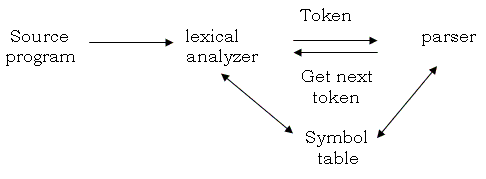
\includegraphics[scale=0.6]{abstract_flow.png}
  \caption{ Процесс работы ПС }
  \label{fig:arch_and_mod::abstract_flow}
\end{figure}


\subsection{Лексический анализатор}
\label{sub:arch_and_mod:lexer}

Так как в дипломном проекте используется синтаксический анализ исходного кода, то, очевидно, для этого анализа должна быть часть, отвечающая за процесс аналического разбора входной последовательности символов. Слово <<лексический>> в традиционном смысле означает <<относящийся к словам>>. С точки зрения языка программирования, слова являются объектами, такими как имена переменных, числа, ключевые слова и т.д. Такие слова традиционно называются <<токенами>>\cite{basic_compiler_design}.

Лексический анализатор, или \textit{лексер}, принимает в качестве входных параметров строку символов, и разделяет эту строку на лексемы. Кроме того, он отфильтровывает все, что разделяет токены, то есть элементы разметки символов (пробелы,переводы строк т.п.) и комментарии.

Основная цель лексического анализа --- упростить процесс последующего синтаксического анализа. В теории, работа, которая проводится во время лексического анализа может
составлять неотъемлемую часть синтаксического анализа, так и в простых системах это действительно почти всегда справедливо. Тем не менее, есть основания для разделения синтаксического и лексического анализа:
\begin{itemize}
\item
  Эффективность: Лексический анализатор может делать простые операции быстрее, чем это делает обычный парсер. Кроме того, размер системы, которая разделена на две части, может
  быть меньше, чем в объединенной системе.
\item
  Модульность: Синтаксическое описание языка не должно быть загромождено мелкими лексическими деталями, такими как пробелы и комментарии.
\item
  Традиция: Языки часто проектируются с отдельными лексическими и синтаксическими анализаторами, а также стандарты таких языков обычно разделяют лексические и синтаксические элементы.
\end{itemize}
\subsubsection{Регулярные выражения}~
\label{sec:arch_and_mod:regex}
Основу лексера, представленного в ПС, составляют регулярные выражения: алгебраическая нотация для описания наборов строк\cite{regular_expressions_tutorial}.

Множество всех целочисленных констант или множество всех имен переменных представляют собой наборы строк, где отдельные буквы берутся из определенного алфавита. Такой набор
строки называется \textit{языком}. Для целых чисел, алфавит состоит из цифр 0-9 и для имен переменных алфавит содержит буквы и цифры (и, возможно, некоторые из них
другие символы, такие как подчеркивание). При заданном алфавите, мы будем описывать наборы строк и обычные выражения. Алгебраическая нотация является компактной и легкой для понимания и использования людьми формой представления. Идея заключается в том, что регулярные выражения, которые описывают простые наборы строк могут быть объединены, чтобы формировать регулярные выражения, которые описывают более сложные наборы строк.

Регулярные выражения разбивают входной поток символов на части, которые затем анализируются, и трансфомируются в токены. Лексер считывает поток символов и останавливается только при встрече определенного символа, называемого \textit{разделителем}. Эти символы уникальны для каждого языка и определены его грамматикой. Разделитель, используемый в программе, а также его использование, приведены в листинге \ref{lst:arch_and_mod:delimiter_usage}:
\begin{lstlisting}[language=Ruby, style=rubystyle,caption={Определение и использование разделителя}, label=lst:arch_and_mod:delimiter_usage]
DELIMITER = '=>|\*\*|:=|\/=|>=|<=|<>|\Z|[&\'()*+,-.\/\:;<=>|\[\]]'
DELIMITER_RE = /(?:#{DELIMITER})/

def parse(str)
  .
  .
  .

  scanner.check_until(/\s|#{DELIMITER}/)
  v = scanner.pre_match[before..-1]
  scanner.pos += v.size
  case v
  when /^abs$/i then
    [:ABS, "abs"]
  when /^access$/i then

  .
  .
  .
end
\end{lstlisting}

Помимо разделителя, в лексере также присутствуют другие регулярные выражения, которые отвечают за определение токены. Эти регулярные выражения и их использование приведены в листинге
\ref{lst:arch_and_mod:literal_usage}:
\begin{lstlisting}[language=Ruby, style=rubystyle,caption={Определение и использование регулярных выражений для опознавания токена}, label=lst:lst:arch_and_mod:literal_usage]
UPPERCASE_LETTERS = 'A-Z'
DIGITS = '0-9'
SPECIAL_CHARS = '\s#&\'\(\)*+,-\.\/\:\;<=>\[\]_|'
SPACE_CHARS = ' '

BASIC_GRAPHIC_CHAR = "#{UPPERCASE_LETTERS}#{DIGITS}#{SPECIAL_CHARS}#{SPACE_CHARS}"
GRAPHIC_CHARS = "#{BASIC_GRAPHIC_CHAR}#{LOWERCASE_LETTERS}#{OTHER_SPECIAL_CHARS}"
BASIC_CHARS = "#{BASIC_GRAPHIC_CHAR}#{FORMAT_EFFECTOR}"

BASIC_IDENT_RE = /[A-Za-z][A-Za-z0-9_]*/
EXTENDED_IDENT_RE = /\\([#{GRAPHIC_CHARS}]+)\\/

INTEGER = '[0-9][0-9_]*'
EXPONENT = 'E[+-]?[0-9][0-9_]*'
BASED_INTEGER  = '[0-9A-Za-z][0-9A-Za-z_]*'
BIT_VALUE = '[0-9A-Za-z][0-9A-Za-z_]*'

DECIMAL_LITERAL_RE = /#{INTEGER}(?:\.#{INTEGER})?(?:#{EXPONENT})?/
BASED_LITERAL_RE = /#{INTEGER}#(?:#{BASED_INTEGER})(?:\.#{BASED_INTEGER})?#(?:#{EXPONENT})?/
CHAR_LITERAL_RE = /'([#{GRAPHIC_CHARS}])'/
STRING_LITERAL_RE = /"([#{GRAPHIC_CHARS}]*)"/
BIT_STRING_LITERAL_RE = /[BOX]"#{BIT_VALUE}"/
COMMENT_RE = /--.*[\r\n]*/
.
.
.
@tokens = s.collect_token{|scanner|
  case
  when scanner.skip(/\s+/)
    # ignore
  when scanner.skip(COMMENT_RE)
    # ignore
  when scanner.scan(EXTENDED_IDENT_RE)
    [:EXTENDED_IDENTIFIER, scanner[1]]
  when scanner.scan(BASED_LITERAL_RE)
    [:BASED_LITERAL, scanner[0]]
  when scanner.scan(DECIMAL_LITERAL_RE)
    [:DECIMAL_LITERAL, scanner[0]]
  when scanner.scan(CHAR_LITERAL_RE)
    [:CHARACTER_LITERAL, scanner[1]]
  when scanner.scan(STRING_LITERAL_RE)
    [:STRING_LITERAL, scanner[1]]
  when scanner.scan(BIT_STRING_LITERAL_RE)
    [:BIT_STRING_LITERAL, scanner[0]]
  when scanner.scan(DELIMITER_RE)
    [scanner[0], scanner[0]]
end
\end{lstlisting}
После того, как встречен разделитель, лексер с помощью регулярных выражений определяет тип лексемы, и если она не является литералом(строковым, символьным, числовыми), проверяется принадлежность строки к набору базовых операторов языка:

\begin{lstlisting}[language=Ruby, style=rubystyle,caption={Проверка принадлежности части строки базовой конструкции языка}]
  .
  .
  .
  before = scanner.pos
  scanner.check_until(/\s|#{DELIMITER}/)
  v = scanner.pre_match[before.0]
  scanner.pos += v.size
  case v
  when /^abs$/i then
    [:ABS, "abs"]
  when /^access$/i then
    [:ACCESS, "access"]
  when /^after$/i then
    [:AFTER, "after"]
  when /^alias$/i then
    [:ALIAS, "alias"]
  when /^all$/i then
    [:ALL, "all"]
  when /^and$/i then
    [:AND, "and"]
  when /^arch$/i then
    [:ARCH, "arch"]
  when /^architecture$/i then
    [:ARCHITECTURE, "architecture"]
  when /^array$/i then
    [:ARRAY, "array"]
  .
  .
  .
end
\end{lstlisting}
Сама лексема представлена как массив, состоящий из 2 элементов: тип лексемы, и ее значение. Пример различных лексем приведен в листинге \ref{lst:arch_and_mod:lexem_definition}:
\begin{lstlisting}[language=Ruby, style=rubystyle,caption={Различные типы лексем}, label=lst:arch_and_mod:lexem_definition]
  .
  .
  .
  when /^xnor$/i then
    [:XNOR, "xnor"]
  when /^xor$/i then
    [:XOR, "xor"]
  else
    [:BASIC_IDENTIFIER, v]
  .
  .
  .
\end{lstlisting}

Данный набор лексем более чем достаточен для исчерпывающего описания языка VHDL. Использование лексера сильно упрощает работу синтаксического анализатора и добавляет ему гибкости, что позволяет расширять его функциональность.
\subsection{Синтаксический анализатор}
\label{sub:arch_and_mod:parser}
Следующий за лексическим анализом шаг --- синтаксический анализ или \textit{парсинг}.

Парсинг --- это процесс структурирования линейного представления в соответствии с заданной грамматикой. ``Линейное представление'' может быть предложением, исходным кодом программы, последовательность геологических слоев, звуковым, файлом, короче говоря, любой линейной последовательностью, в которой предыдущие элементы некоторым способом предопределяют следующий элемент.

В дополнение к поиску структуры входного текста, синтаксический анализ должен также отвергать недействительные тексты, сообщая о синтаксических ошибках. Поскольку синтаксический анализ имеет менее локальный характер, для него требуются более продвинутые методы. В нашем случае используется та же базовая стратегия: нотация, пригодная для чтения человеком, трансформируется в машинную низкоуровневую нотацию, которая подходит для эффективного выполнения. Этот процесс называется генерацией синтаксического анализатора.

Нотация которая используется для манипуляций человека является контекстно-свободной грамматикой, которая является рекурсивным обозначением для описания наборов строк и наложения структуры на каждую такую строки. Эти нотации могут в некоторых случаях быть переведены непосредственно в рекурсивные программы, но часто бывает удобнее перевести их в конечный автомат стекового типа. Они похожи на конечный автомат, используемый для лексического анализа, но они могут дополнительно использовать стек, который позволяет считать и находить соответствия вне локального контекста.
\subsubsection{Контексто-независимые грамматики}~
\label{sub:arch_and_mod:grammars}

Подобно регулярным выражениям, контекстно-независимые грамматики описывают наборы строк, то есть \textit{языки}. Кроме того, контекстно-независимая грамматика также определяет структуру над строками в определяемом языке. Язык определен над некоторым алфавитом, например, набор токенов, полученных с помощью лексера или набор буквенно-цифровых символов. Символы в алфавите называются \textit{терминалами}. Контекстно\hyphнезависимая грамматика рекурсивно определяет несколько наборов строк. Каждый набор обозначается именем, которое называется \textit{нетерминалом}. Множество нетерминалов не пересекается с другим множеством нетерминалов. Один из нетерминалов выбирается для обозначения языка, описываемого грамматикой. Это называется стартовым символом грамматики. Множества описываются рядом продукций(production rule). Каждая продукция описывает некоторые из возможных строк, содержащихся в наборе, обозначенном нетерминалом. Продукция имеет вид
\begin{equation}
  N \rightarrow X_1...X_n
\end{equation}
\begin{explanation}
где N - нетерминал, $X_1...X_n$ - 0 или более символов, каждый из которых \\
    является или терминалом, или нетерминалом
\end{explanation}

Предполагаемый смысл этого обозначения в том, что множество обозначаемое через $N$ содержит строки, которые получаются с помощью конкатенации строк из множеств, обозначенных
$X_1...X_n$. В данном случае терминал обозначает одноэлементный набор, так же, как алфавит символов в регулярных выражениях, например:

\begin{equation}
  A \rightarrow a
\end{equation}
\begin{explanation}
описывает набор, обозначенный нетерминалом $A$, который содержит строку \\
из одного символа $a$
\end{explanation}

\begin{equation}
  A \rightarrow aA
\end{equation}
\begin{explanation}
обозначает, что множество, обозначенное как $A$, содержит все строки,\\
образованные добавлением символа $a$ в начало строки, взятой из \\ множества $a$
\end{explanation}
Можно определить  грамматику, эквивалентную регулярному выражению $a*$ с помощью двух продукций:
\begin{equation}
\begin{aligned}
  &B \rightarrow        \\
  &B \rightarrow aB
\end{aligned}
\end{equation}
\begin{explanation}
где первая продукция показывает, что пустая строка является частью \\
множества $B$.
\end{explanation}

Для каждой грамматики, существует, как правило, бесконечное число линейных представлений
("предложений"), которые могут быть представлены ей. То есть, грамматика конечного размера может соответствовать бесконечному числу предложений. Это основное преимущество грамматик
и доказательство их важности: они обобщают структуру бесконечного числа объектов определенного класса.
Есть несколько причин, чтобы выполнить процесс парсинга. Одна из
причин вытекает из того факта, что полученная структура помогает нам обрабатывать объект
в дальнейшем. Когда мы знаем, что определенный сегмент предложения на немецком языке является предметом,
эта информация помогает в переводе предложения. После того, как структура документа обработана синтаксическим анализатором, манипулировать ей становится в разы проще.
\subsubsection{Генератор парсеров YACC}~
\label{sub:arch_and_mod:parser_generator}
Посколько разработка собственного парсера является очень затратной, было принято решение использовать генератор парсеров. Генератор парсеров --- приложение, которое генерирует исходный код LALR(1)-парсера на основе BNF грамматик. Акроним LALR расшифровывается как lookahead left-right. Цифра ``1'' означает, на сколько символов вперед смотрит анализатор. Для написания был использован адаптер YACC(yet another compiler compiler) для языка ruby --- RACC. В качестве правил использовалась модифицированная BNF грамматика для языка VHDL и уникальный набор действий для каждого правила. Пример грамматики приведен в листинге \ref{lst:arch_and_mod:yacc_rules}:
\begin{lstlisting}[language=Ruby, style=rubystyle,caption={Различные описания грамматик и действия, вызываемые при соответствии грамматики линейной последовательности}, label=lst:arch_and_mod:yacc_rules]
  .
  .
  .
abstract_literal :
  DECIMAL_LITERAL {
    result = DecimalLiteral.new(val[0]);
    LiteralRepository.add(result);
  }
  | BASED_LITERAL {result = val[0]}

access_type_definition :
  ACCESS subtype_indication {result = val}

actual_designator :
  expression {result = val[0]}
  | signal_name {result = val[0]}
  | variable_name {result = val[0]}
  | file_name {result = val[0]}
  | OPEN {result = val[0]}

expression :
  relation expression_loop0 {result = Expression.new(val.flatten); }
  | STRING_LITERAL {result = StringLiteral.new(val[0]);}
  | relation expression_loop1 {result =  Expression.new(val.flatten);}
  | relation expression_loop2 {result =  Expression.new(val.flatten);}
  | relation NAND relation {result =  Expression.new(val.flatten);}
  | relation NOR relation {result =  Expression.new(val.flatten);}
  | relation expression_loop3 {result =  Expression.new(val.flatten);}

  .
  .
  .
\end{lstlisting}
Поскольку грамматики описываются в форме Бэкуса---Наура, то эти правила могут рекурсивными:


\begin{lstlisting}[language=Ruby, style=rubystyle,caption={Пример рекурсивных правил}, label=lst:arch_and_mod:recursive_rules]
  identifier_list :
    identifier identifier_list_loop0 {result = val = IdentifierList.new(val.flatten); InitializeRepository.add(result.identifiers) }

  identifier_list_loop0 :
    ',' identifier identifier_list_loop0 {result = val - [',']}
    | {result = val}
\end{lstlisting}


Подобно другим сдвиго-сверточным анализаторам, LR-парсер ожидает сканирования следующего символа и пытается сделать свертку в некую конструкцию всех элементов на стеке. Как только найдено правило для заданных элементов, парсер немедленно сворачивает конструкцию. В примере в таблице \ref{arch_and_mod:parse_table}, литерал \textit{A} сворачивается до \textit{Значения}, а затем до \textit{Умножения} (согласно имени правила) на шагах 1-3 как только следующий(lookahead) символ ``*''  виден, а не ждет дополнительных комманд, чтобы организовать эти части дерева. Решения, как  обрабатывать литерал \textit{A} базируются только на том, что сканнер и парсер уже видели, не принимая в расчет те элементы, что будут прочтены позднее.
Свертка реорганизует последние проанализириванные элементы непосредственно слева от следующего символа. Поэтому список проанализированных элементов является стеком. Стек растет слева-направо. Вершина стека находится левее всех и содержит старейший проанализированный фрагмент. Каждый шаг свертки действует только на крайнем правом, новейшем фрагменте.
Пример обработки выражения $A*2+1$ приведен в таблице \ref{arch_and_mod:parse_table}:

\begin{table}[ht]
  \caption{Пример разбора выражения $A*2+1$}
  \label{arch_and_mod:parse_table}
  \begin{tabular}{| >{\centering}m{0.07\textwidth}
                  | >{\centering}m{0.23\textwidth}
                  | >{\centering}m{0.2\textwidth}
                  | >{\centering}m{0.4\textwidth}|}
  \hline
  Шаг & Cтек парсера & Выражение & Сдвиг/Свертка \tabularnewline
  \hline
  0 & empty & $A*2+1$ & Cдвиг \tabularnewline
  \hline
  1 &  id  & $*2 + 1$ & Значение $\rightarrow $ id \tabularnewline
  \hline
  2 &  Value &  $*2 + 1$ & Products $\rightarrow $ Value \tabularnewline
  \hline
  3 &  Products & $*2 + 1$ & Сдвиг \tabularnewline
  \hline
  4 &  Products  * &  $2 + 1$  & Сдвиг \tabularnewline
  \hline
  5 &  Products  * int &$  + 1$  & Value $\rightarrow $ int \tabularnewline
  \hline
  6 &  Products  * Value &  $+ 1$ &  Products $\rightarrow $ Products * Value \tabularnewline
  \hline
  7 &  Products & $+ 1$  &  Sums $\rightarrow $ Products \tabularnewline
  \hline
  8 &  Sums & $+ 1$  & Сдвиг \tabularnewline
  \hline
  9 &  Sums  + &  $1$  & Сдвиг \tabularnewline
  \hline
  10 & Sums  + int &  eof &  Value $\rightarrow $ int \tabularnewline
  \hline
  11 & Sums + Value & eof &   Products $\rightarrow $ Value \tabularnewline
  \hline
  12 & Sums + Products &  eof  & Sums $\rightarrow $ Sums + Products \tabularnewline
  \hline
  13 & Sums & eof &  done \tabularnewline
  \hline
  \end{tabular}
\end{table}


На рисунке~\ref{fig:arch_and_mod::lr_example_img} представлено состояние парсера на одном из шагов:

\begin{figure}[!htb]
  \centering
  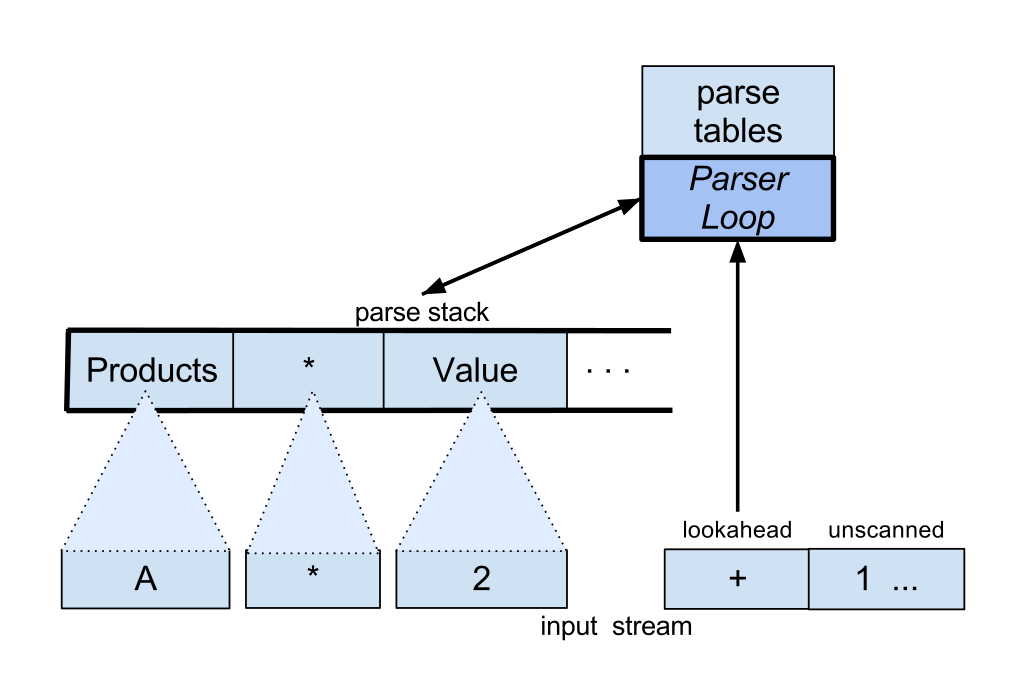
\includegraphics[scale=0.3]{parser_state.png}
  \caption{ Состояние парсера на шаге №6 }
  \label{fig:arch_and_mod::lr_example_img}
\end{figure}

\FloatBarrier


\subsubsection{Абстрактное синтаксическое дерево}~
\label{sub:arch_and_mod:ast}
Каждое правило содержит действие, которое выполнится при соответствии оного. В данном ПС эти действия на построение абстрактного синтаксического дерева(Abstract syntax tree, AST), которое представляет собой структуру программы в удобном виде, с возможностью модификации узлов, что является необходимым условием для обфускации исходной последовательности.

Абстрактное синтаксическое дерево --- это конечное, помеченное, ориентированное дерево, в котором внутренние вершины сопоставлены с операторами языка программирования, а листья --- с соответствующими операндарми. Таким образом, листья являются пустыми операторами и представляют только переменные и константы.

Для языка, который описывается контекстно-независимой грамматикой, какими являются почти все языки программирования, создание абстрактного дерева в синтаксическом анализаторе является тривиальной задачей. Большинство правил в грамматике создают новую вершину, а символы в правиле становятся ребрами. Правила, которые ничего не привносят в АСД(например, группирующие правила), просто заменяются в вершине одним из своих символов. Кроме того, анализатор можешт создать полное дерево разбора и затем пройти по нему, удаляя узлы и рёбра, которые не используются в абстрактном синтаксисе, для получения АСД.

Структура АСД часто тесно связана с дизайном компилятора и его ожидаемых функций.
Основные требования включают в себя следующее:
\begin{itemize}
\item  Типы переменных должны быть сохранены, а также расположение каждого объявления в исходном коде.
\item  Порядок исполняемых операторов должен быть явно представлены и четко определен.
\item  Левая и правая компоненты бинарных операций должны храниться и правильно определены.
\item  Идентификаторы и назначенные им значения должны быть сохранены для операторов присваивания.
\end{itemize}

Некоторые операции всегда будут требовать двух элементов, таких, как два слагаемых для операции суммирования. Тем не менее, некоторые языковые конструкции требуют сколь угодно большого числа операндов, таких как списки аргументов, передаваемых программе из командной оболочки. В результате, АСД используется для представления кода, написанного на таком языке, который должен быть достаточно гибким, чтобы позволить быстрое добавление неизвестного количества детей(листьев дерева).
Еще одним желательным условием конструкции для АСД является то, что должна быть обеспечена возможность представления АСД в виде исходного кода. Исходный код, сгенерированный из АСД, должен быть достаточно похожим на оригинал по внешнему виду и идентичным в исполнении. Последнее является обязательным, так как после обфускации дерева его необходимо перевести в исходный код.

\subsection{Обфускатор}
\label{sub:arch_and_mod:grammars}

После того, как сформировано синтаксическое дерево, необходимо внести в его изменения. В данном ПС обфускатором представлен наборов классов-оболочек над примитивами языка VHDL и контейнерами литералов.
Т.к мы используем генератор парсеров, то обфускатор инициализируется на этапе синтаксического анализа(создаются экземпляры классов, создаются соответствия между реальными именами переменных и их обфусцированными вариантами). Сам процесс обфускации реализован через определение метода \textbf{to\_s}  у классов-оболочек, что позволяет автоматически заменять имена переменных, вставлять произвольный код прямо в процессе конвертации экземпляра класса в строку:

\begin{lstlisting}[language=Ruby, style=rubystyle,caption={Определение метода перевода класса в строку для примитива component instantiation}, label=lst:arch_and_mod:wrapper_to_s]
  def to_s
    "#{@name} : #{@instantiated_unit} #{@generic_map_aspect}#{@port_map_aspect ? '' : ';'}#{@port_map_aspect}"
  end
\end{lstlisting}


\subsubsection{Контейнеры литералов}~
  Контейнеры литералов представлены в виде трёх классов для различных видов литералов:
  \begin{itemize}
  \item InitializerRepository --- контейнер для хранения строковых литералов. Является статическим, содержит в себе все строковые литералы, объявленные в программе, такие как имена переменных, сигналов, процессов, архитектур. При добавлении нового литерала для него автоматически создаётся его обфусцированное соответствие:
  \begin{lstlisting}[language=Ruby, style=rubystyle,caption={Определение метода перевода класса в строку для примитива component instantiation}, label=lst:arch_and_mod:initializer_repository_add]
    def self.add identifier
      identifier = [identifier] unless identifier.is_a? Array
      @@initializers.push identifier
      @@initializers.flatten!
      @@initializers.uniq!(&:name)
      identifier.each{|i| generate_mapping_for(i)}
    end
  \end{lstlisting}

  Как видно из листинга \ref{lst:arch_and_mod:initializer_repository_add}, список литералов их соответствия являются уникальными, так как многие из них используются несколько раз(например, при объявлении архитектуры и при её окончании).
  Контейнер имеет ряд вспомогательных методов, которые используются сторонними классами для определения, существует ли соответствие для данного литерала и метод выдачи соответствия по имени литерала:

  \begin{lstlisting}[language=Ruby, style=rubystyle,caption={Вспомогательные методы контейнера}, label=lst:arch_and_mod:support_methods]
    def self.mapping_defined? identifier
      !!@@mappings[identifier]
    end

    def self.mapping_for identifier
      @@mappings[identifier]
    end
  \end{lstlisting}
  \item
  LiteralRepository --- контейнер для хранения числовых и символьных литералов. Этот контейнер имеет специфическое поведение, так как конкретные числа или символы невозможно поставить в соответствие некоторому строковому литералу. Поэтому у этих литералов существует дополнительный метод \textbf{stringified}, уникальный, для каждого типа литерала:
  \subitem Для числовых литералов:
    \begin{lstlisting}[language=Ruby, style=rubystyle,caption={Вспомогательные метод stringified для числовых литералов}, label=lst:arch_and_mod:decimal_stringified]
      def stringified
        @value.to_i
      end
    \end{lstlisting}
  \subitem Для строковых литералов:
     \begin{lstlisting}[language=Ruby, style=rubystyle,caption={Вспомогательные метод stringified для символьных литералов}, label=lst:arch_and_mod:character_stringified]
      def stringified
        "'#{@value}'"
      end
    \end{lstlisting}
  Контейнер ищет соответствие по значению, возвращаемому этой функцией. Это сделано для того, чтобы избежать возможных коллизий, так как в синтаксическом анализаторе все числа и символы представлены строкой из одного символа, поэтому возможен конфликт типов при одновременном существовании в исходном коде символьных литералов '0' и '1' и соотвествующих числовых литералов.
  \item
  ConstantValueRepository --- контейнер для хранения константных значений. Этот контейнер уникален тем, что используется для функциональной обфускации: вместо генерации текстового соответствия, этот контейнер генерирует определение сигнала, которое затем добавляется в определения архитектуры и соответствующий примитив для замены оригинального значения:
  \begin{lstlisting}[language=Ruby, style=rubystyle,caption={Создание сигнала на основе значения константы}, label=lst:arch_and_mod:constant_generate_name]
    .
    .
    .
    @@signals << SignalDeclaration.new('SIGNAL', name, nil, TypeWrapper.new(literal.type, nil, true), nil)
    wires = AssociationList.new([AssociationElement.new('src', name), AssociationElement.new('q', name)])
    port_map_aspect = PortMap.new('PORT', wires)
    if literal.value == '1'
      @@statements << ComponentInstantiation.new(attr_name, 'cvg_1', nil, port_map_aspect);
    else
      @@statements << ComponentInstantiation.new(attr_name, 'cvg_2', nil, port_map_aspect);
    end
    .
    .
    .
  \end{lstlisting}
  \end{itemize}

Все 3 контейнера реализуют метод генерации случайного имени, представленный в листинге~\ref{lst:arch_and_mod:generate_name}
  \begin{lstlisting}[language=Ruby, style=rubystyle,caption={Вспомогательные метод stringified для символьных литералов}, label=lst:arch_and_mod:generate_name]
    def self.generate_random_name(size: rand(6..10), alphabet: %w{ 2 3 4 6 7 9 A C D E F G H J K M N P Q R T V W X Y Z})
      charset = alphabet
      reduced_charset = charset.reject{|x| x =~ /\d/}

      reduced_charset[rand(reduced_charset.size)] + (1...size).map{ charset.to_a[rand(charset.size)] }.join
    end
  \end{lstlisting}
Три данные класса составляют существенную часть обфускатора, так как реализуют базовый функционал, которым управляют классы-оболочки.




\subsubsection{Классы-оболочки}~реализуют базовые примитивы языка VHDL. В данном ПС представлено 32 класса, экземпляры которых при конвертации в строку представляют копию исходного кода, на основе которого был создан экземпляр. Поскольку структура проанализированного кода представляет собой дерево, классы более высшего порядка принимают в качестве аргументов классы, описывающие меньшие порядки или терминальные элементы(контейнеры литералов). Ниже представлен список классов высокого порядка:
\begin{itemize}
\item класс DesignFile является классом высшего порядка(корнем синтаксического дерева), содержащим в себе все выражения дерева. Принимает только один аргумент: набор выражений, однако играет очень важную роль в функциональной обфускации, так как именно на этом этапе добавляются дополнительные примитивы, необходимые для запутывания схемы на  уровне RTL:
  \begin{lstlisting}[language=Ruby, style=rubystyle,caption={Добавление дополнительных компонентов для функциональной обфускации}, label=lst:arch_and_mod:design_functional_obf]
    def generalize_literals
      .
      .
      .
      @statements.unshift(cvg_1, cvg_2)
      header = @statements.select {|s| s.class.name == 'EntityDeclaration'}[0].header

      unless header.is_a? Array
        header = [header]
      end
      generic_clause = nil

      append_to_header = false
      if header[0] && header[0].class.name == 'GenericClause'
        generic_clause = header[0]
      else
        generic_clause = GenericClause.new([])
        append_to_header = true
      end

      generic_clause.generics.each do |statement|
        if statement.class.name == 'SignalDeclaration'
          statement.value = statement.assigned_value
        end
      end
      statements = []

      LiteralRepository.literals.each do |literal|
        signal = SignalDeclaration.new(nil, LiteralRepository.mapping_for(literal.stringified), nil, TypeWrapper.new(literal.type, nil, true), literal.stringified)
        generic_clause.generics.unshift signal
      end

      generic_clause.generics.last.type.append_semicolon = false

      (@statements.select {|s| s.class.name == 'EntityDeclaration'}[0].header = [generic_clause,header].flatten) if append_to_header
    end
  \end{lstlisting}
\item класс EntityDeclaration содержит в себе описание структуры сущности. Сущность содержит в себе порты, константы, <<дженерики>>.
\item класс ArchitectureDeclaration описывает дизайн архитектуры. Класс принимает имя архитектуры, имя сущности, набор определений(объявления переменных, сигналов), набор операторов, и закрывающую часть(посколько VHDL имеет различные формы закрывающих конструкций). Экземпляр этого класса создаётся каждый раз, когда грамматике \textit{architecture\_declaration} находится соответствие. Кроме того, именно в этом классе добавляются дополнительные определения, созданные функциональные обфускатором:
  \begin{lstlisting}[language=Ruby, style=rubystyle,caption={Часть кода, отвечающая за функциональную обфускацию}, label=lst:arch_and_mod:declaration_functional_obf]
    class ArchitectureDeclaration

      attr_accessor :type, :identifiers
      def initialize(arch_name, entity_name, declarative_part , statement_part, closing_part)
        @name = arch_name
        @entity = entity_name
        @declarations = declarative_part
        @statements = statement_part
        @closing_part = closing_part.join(' ')
        obfuscate_literals
      end

      def obfuscate_literals
        @declarations.unshift(*ConstantValueRepository.signals)
        @statements.unshift(*ConstantValueRepository.statements)
      end
      .
      .
      .
  \end{lstlisting}
\item класс ProcessDeclaration описывает оператор процесса. Оператор процесса --- параллельный оператор, представляющий основу языка VHDL. Объявленными в процессе могут быть: объявление и тело подпрограммы, объявление типа и подтипа, объявление константы, переменной, файла, псевдонима, объявление и спецификация атрибута, объявление группы, описание use. То, что объявлено в процессе, имеет область действия (видимость), ограниченную данным процессом. Принимает в качестве параметров модифкатор процесса(POSTPONED или отсутствует), метку процесса, список чувствительности, объявления(сигналов, подпрограмм, переменных и т.д), набор операторов, закрывающую часть(аналогично классу \\ArchitectureDeclaration). Учавствует в функциональной обфускации: список чувствительности должен содержать сигналы, описанные в генераторах константных значений.
\end{itemize}
% \subsection{Представление вероятностной сети}

% Другой важной частью разработанной библиотеки являются типы для представления и работы с самими вероятностными сетями.
% Первостепенными требованиями, поставленными перед началом проектирования типов, были следующие пункты:
% \begin{itemize}
%   \item Типы предназначены для представления модификации классических байесовых сетей, упомянутой в разделе~\ref{sub:domain:bayes_net} на странице~\pageref{page:domain:bayes_mod}.
%   \item Представление сети должно быть <<многослойным>>.
%   Под <<многослойностью>> понимается возможность расширения представления сети дополнительными <<слоями>> атрибутов, с целью увеличения количества сценариев, в которых данные типы пригодны к использованию.
%   Например, в случае когда нужно знать лишь структуру сети можно использовать лишь информацию о структуре "--- граф.
%   Для проведения статистического вывода суждений добавляется дополнительный <<слой>>, содержащий талицы условных и безусловных вероятностей.
%   В случаях, когда нужно отображать сеть пользователю, добавляется еще один <<слой>>, содержащий дополнительную информацию о переменных и их состояниях.
%   \item Сеть должна предоставлять возможность отмены вносимых в нее изменений, т.\,е. по сути поддерживать версионность.
%   \item Сеть должна предоставлять возможность валидации её структуры.
% \end{itemize}

% Приняв во внимание приведенные выше требования были приняты следующие решения:
% \begin{itemize}
%   \item Необходимо разработать отдельные типы для представления вершин вероятностной модели и связей между переменными в этой модели.
%   В разработанной библиотеке за это отвечают типы \lstinline!Node<'T>! и \lstinline!Link<'T>!, содержащие информацию о переменных, таблицы распределения и дополнительные атрибуты.
%   Использование параметрического полиморфизма в реализации данных типов играет ключевую роль в обеспечении <<многослойности>> и расширяемости представления вероятностной сети.
%   \item Необходимы типы для представления распределения.
%   В предложенной реализации был разработан тип для представления безусловного распределения случайной величины, эта таблица хранится в сети как один из аттрибутов типа \lstinline!Node<'T>!, и тип для представления условного распределения пары случайных величин, экземпляр данного типа хранится как аттрибут связи между переменными "--- \lstinline!Link<'T>!.
%   Было сочтено целесообразным в качестве внутренней реализации таблиц распределения использовать готовую библиотеку для работы с матрицами и другими математическими объектами и понятиями "--- Math.NET Numerics\footnote{\url{http://numerics.mathdotnet.com/}}.
%   Соответственно в предложенной реализации использовались типы \lstinline!Vector<float>! и \lstinline!Matrix<float>! и сопутствующие операции над ними.
%   Использование данной библиотеки позволило сократить объём сопутствующего кода, необходимого для реализации библиотеки для работы с вероятностными сетями, также уменьшив множество потенциальных ошибок реализации.
%   В данном случае преимущества от использования библиотеки превысили затраты на добавление и поддержку дополнительных зависимостей.

%   \item Требование возможности отмены изменений вносимых в вероятностную сеть привело к реализации сети, как и в случае типов для представления графов, к реализации сети как неизменяемой структуры данных.
%   Все операции, при условии использования специальных функций, возвращают новый экземпляр сети, оставляя старый не изменённым.
%   Подобная реализация типов автоматически дает возможность производить версионирование экземпляров типа, т.\,к. всегда есть доступ к изменённой копии и исходному экземпляру.
%   С первого взгляда данный подход кажется очень расточительным по памяти, но на самом деле оказывается, что все с точностью до наоборот, т.\,к. обычно, и в данном конкретном случае, при модификации неизменяемой структуры данных большая часть структуры разделяется между копией и исходной структурой, а физически копирование памяти происходит лишь в тех местах, которые действительно необходимо было поменять.
%   Для убедительности, сказанное проиллюстрировано на рисунке~\ref{fig:arch_and_mod:probab_net:immutable_ds_modification}.

%   \item Валидация сети происходит на этапе её построения и модификации.
%   Дополнительно существуют функции для проверки структуры сети на ацикличность.
%   Ацикличность ориентированного графа проверяется с помощью алгоритма нахождения компонент сильной связности Косарайю\footnote{\url{http://en.wikipedia.org/wiki/Kosaraju's_algorithm}}.

% \end{itemize}

% \begin{figure}[ht]
% \centering
%   \begin{subfigure}[b]{0.41\linewidth}
%     \centering
%     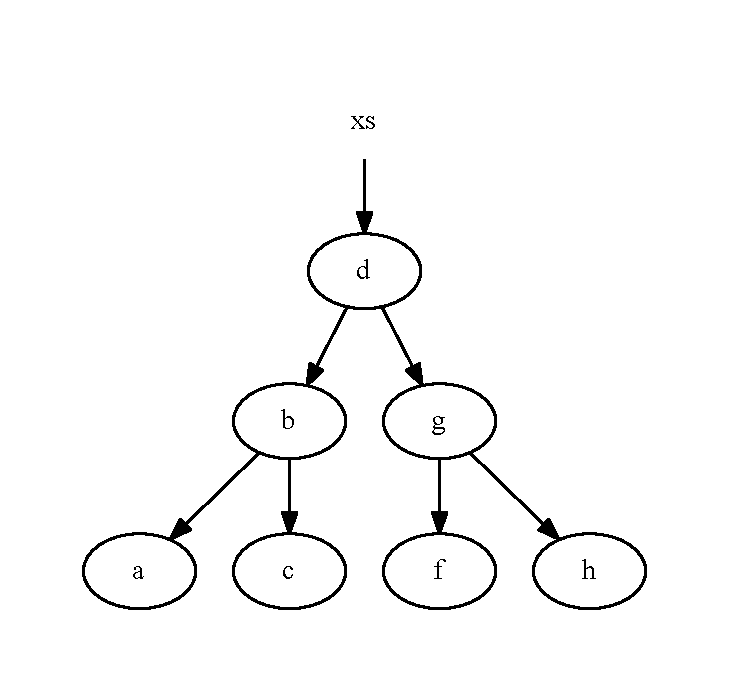
\includegraphics[scale=0.63]{persistent_tree.pdf}
%     \caption{}
%   \end{subfigure}
%   \begin{subfigure}[b]{0.58\linewidth}
%     \centering
%     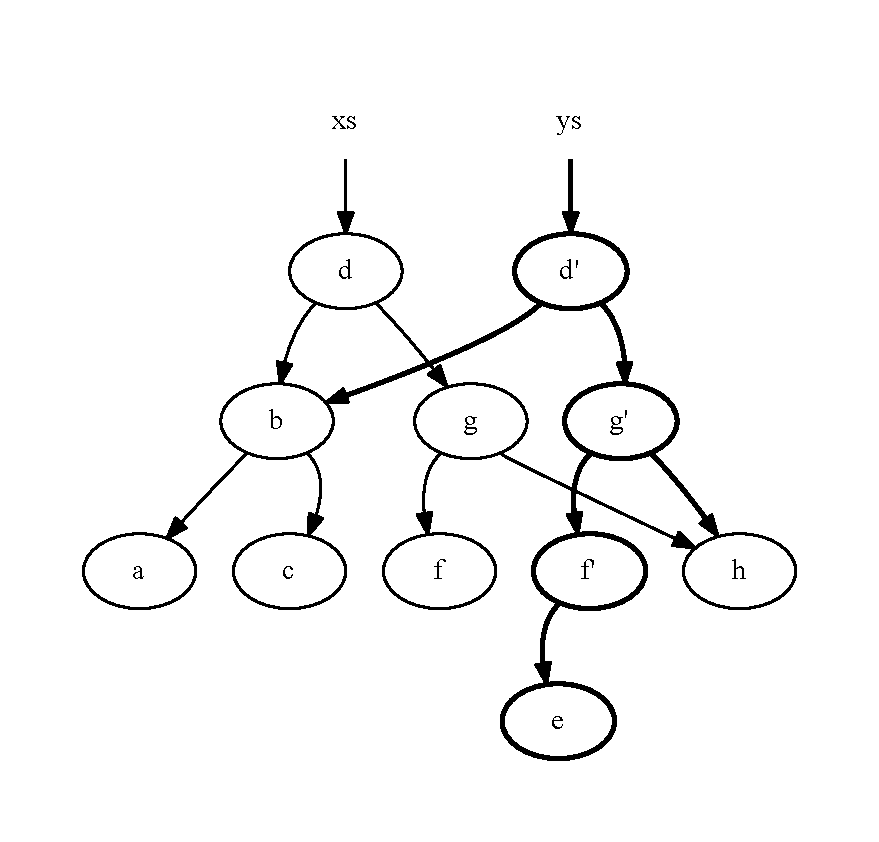
\includegraphics[scale=0.63]{persistent_tree_mod.pdf}
%     \caption{}
%   \end{subfigure}
%   \caption{ Пример разделения структуры в неизменяемых структурах данных:
%             а "--- исходное дерево;
%             б "--- измененное дерево, добавлена вершина \textit{e};}
%   \label{fig:arch_and_mod:probab_net:immutable_ds_modification}
% \end{figure}

% В результате получилось довольно простое и расширяемое представление сети, основное определение которого приведено в листинге~\ref{lst:arch_and_mod:probab_net:bnet_definition}.
% Параметризация типа параметрами \lstinline!'NodeAttributes! и \lstinline!'LinkAttributes! и расширяемое устройство типов \lstinline!Node<'T>! и \lstinline!Link<'T>! позволяет достигнуть заявленной расширяемости представления сети и её <<многослойности>>.
% Библиотека содержит предопредёленные типы, для представления уровней.
% Параметризация типа \lstinline!BNet<unit, unit>! представляет структуру сети и таблицы распределения.
% <<Слой>> с дополнительными аттрибутами, планируемыми для использования в алгоритмах статистического вывода суждений представлен типами \lstinline!NodeAttributes<'Annotations>! и \lstinline!LinkAttributes!, но на момент защиты дипломного проекта, из-за неготовой реализации алгоритмов статистического вывода суждений, данные типы содержат не все необходимые атрибуты для работы таких алгоритмов, а лишь прогнозируемых заготовки.
% Дополнительный <<слой>>, потенциально необходимый при построении пользовательских приложений, представлен типом \lstinline!VarAnnotations!.
% Данный тип содержит дополнительную информацию о переменной, такую как её название и аннотации возможных значений переменной.
% Таким образом, наиболее полное представление сети, содержащее все <<слои>>, в коде параметризуется следующим образом \lstinline!BNet<NodeAttributes<VarAnnotations>, LinkAttributes>!.

% \begin{lstlisting}[style=fsharpstyle,caption={Определение структуры данных для вероятностной сети}, label=lst:arch_and_mod:probab_net:bnet_definition]
% /// Represents immutable BN. Nodes and links between nodes.
% type BNet<'NodeAttributes, 'LinkAttributes> =
%     private { nodes: Map<int, Node<'NodeAttributes>>;
%               links: Map<int * int, Link<'LinkAttributes>>;
%               graph: Graph<int, unit>; }
% \end{lstlisting}

% Таким образом, использование параметрического полиморфизма и не\-изменяемых типов данных, позволило добиться поставленных при проектировании целей, а также довольно легкой возможности расширять сеть в дальнейшем.

% \subsection{Сохранение сети} % (fold)
% \label{sub:arch_and_mod:net_persistence}

% Помимо функциональности, связанной с представлением, манипуляцией и выведением структуры сети, разработанная библиотека предоставляет возможность импорта и экспорта вероятностной сети из и в различные форматы.
% Т.\,к. библиотека предназначена для работы с модификацией вероятностных сетей, отличающейся в нескольких ключевых моментах от классических байесовых сетей, то нельзя было использовать общепринятые форматы для хранения сетей во внешней памяти и необходимо было разработать свой формат.
% Разработанный формат хранения сетей основывается на XML и предназначен для полного сохранения состояния представления сети, используемого в программе.
% Данный формат в большей степени похож на ручную сериализацию, чем на удобный формат для обмена вероятностными сетями.
% Пример сети, представленной в данном формате, приведен в листинге~\ref{lst:arch_and_mod:net_persistence:bnxml}.

% У разработанного формата есть существенный недостаток, его <<понимает>> только разработанная библиотека.
% В связи с тем, что в данном дипломном проекте основной целью является реализация лишь малой части возможных операций над вероятностными сетями "--- построение структуры по данным, целесообразно было добавить в библиотеку, хотя и весьма ограниченную, возможность загрузки и сохранения вероятностных сетей из и в существующие распространённые форматы.
% Список поддерживаемых форматов приведён в таблице~\ref{table:arch_and_mod:net_persistence:supported_formats}.
% Поддержка нескольких форматов понадобилась потому, что многие существующие программы, которые использовались в различной степени для оценки результатов проделанной работы, поддерживают весьма ограниченный набор форматов.
% Таким образом, имея возможность экспортировать сеть, построенную одним из алгоритмов реализованных в разработанной библиотеке по данным, в общеиспользуемый формат можно использовать обученную сеть для статистического вывода суждений и других операций в существующих программах, т.\,к. в данный момент в разработанной библиотеке данная функциональность не реализована.
% Отдельно стоит отметить возможность сохранения структуры сети в формат представления графов программы GraphViz\footnote{\url{http://www.graphviz.org/}}.
% Данное ПО использовалось с целью визуализации выведенных структур и экспорта полученной визуализации в один из векторных графических форматов.
% Утилита dot из состава GraphViz умеет автоматически визуализировать сложные графы наилучшим для отображения образом.

% \clearpage
% \begin{lstlisting}[language=XML,caption={Пример представления простой вероятностной сети в собственном XML"=формате}, label=lst:arch_and_mod:net_persistence:bnxml]
% <network>
%   <variables>
%     <variable id="1" dim="2" />
%     <variable id="2" dim="3" />
%   </variables>
%   <node_attributes>
%     <node variable_id="1"> <answered>false</answered> </node>
%     <node variable_id="2"> <answered>true</answered>  </node>
%   </node_attributes>
%   <link_attributes>
%     <link parent_id="1" child_id="2" />
%   </link_attributes>
%   <variable_annotations>
%     <variable_annotation variable_id="1">
%       <name>My variable</name>
%       <annotations>
%         <label>Yes</label> <label>No</label>
%       </annotations>
%     </variable_annotation>
%     <variable_annotation variable_id="2">
%       <name>Color</name>
%       <annotations>
%         <label>Red</label> <label>Green</label> <label>Blue</label>
%       </annotations>
%     </variable_annotation>
%   </variable_annotations>
%   <probability_tables>
%     <probability_table variable_id="1">
%       <vector>0.2 0.8</vector>
%     </probability_table>
%     <probability_table variable_id="2">
%       <vector>0.4 0.3 0.3</vector>
%     </probability_table>
%   </probability_tables>
%   <forward_probability_tables>
%     <forward_probability_table variable_id="2" condition_variable_id="1">
%       <matrix nrows="3" ncols="2">0.1 0.2 0.7 0.6 0.1 0.3</matrix>
%     </forward_probability_table>
%   </forward_probability_tables>
% </network>
% \end{lstlisting}

% \begin{table}[ht]
% \caption{Поддерживаемые форматы хранения вероятностных сетей}
% \label{table:arch_and_mod:net_persistence:supported_formats}
% \centering
%   \begin{tabular}{| >{\raggedright}m{0.35\textwidth}
%                   | >{\centering}m{0.27\textwidth}
%                   | >{\centering\arraybackslash}m{0.27\textwidth}|}
%   \hline Формат & Поддержка импорта & Поддержка экспорта \\
%   \hline Собственный xml"=формат & полная & полная \\
%   \hline XMLBIF & частичная & частичная \\
%   \hline GeNIe & частичная & отсутствует \\
%   \hline GraphViz dot & отсутствует & полная \\
%   \hline
%   \end{tabular}
% \end{table}



% \subsection{Представление экспериментальных данных}
% \label{sub:arch_and_mod:dataframe}

% Немаловажной задачей в обучении и построении структуры сети по данным является представление набора экспериментальных данных в оперативной и постоянной памяти.
% В машинном обучении и других областях, связанных с обработкой массивов данных, для хранения данных на диске в большинстве случаев применяется простой текстовый формат \emph{csv} "--- значения, разделённые специальным символом и записанные в текстовый файл построчно.
% В разработанной библиотеке также используется данный формат для импортирования экспериментальных данных с диска в память программы для дальнейшей обработки.
% Для чтения \emph{csv} файлов используется легковесная внешняя библиотека LumenWorks.Framework.IO\footnote{\url{http://www.codeproject.com/Articles/9258/A-Fast-CSV-Reader}}.

% Для представления набора экспериментальны данных в библиотеке присутствует специальный тип "--- DataFrame, который представляет из себя информацию о переменных и, собственно, набор экспериментальных данных в компактном для хранения виде.
% Из особенностей реализации стоит упомянуть способ достижения компактности хранения.
% При чтении \emph{csv} файла каждому состоянию переменной назначается некоторое 8-битное число, которое является представлением данного состояния в памяти компьютера.
% Использование 8"=битного числа с одной стороны ограничивает число возможных состояний одной переменной до \num{256}, с другой стороны "--- данное представление достаточно компактно, чтобы быть пригодным для работы на персональном компьютере разработчика с ограниченным размером ОЗУ и уметь обрабатывать наборы данных из миллионов случаев для десятков переменных.
% Одной из дополнительных возможностей DataFrame является возможность производить случайные выборки из имеющегося набора данных.
% Данная возможность была использована при реализации алгоритмов вывода структуры вероятностной сети по данным.


% \subsection{Байесовы сети Asia и ALARM}
% \label{sub:arch_and_mod:asia_and_alarm}

% Перед тем как перейти к обсуждению разработанных алгоритмов вывода структуры сети по данным целесообразно обсудить известные сети, которые использовались в качестве моделей для вывода по экспериментальным данным.
% Речь пойдет о ставших уже классикой в таких задачах "--- сетях Asia и ALARM.

% \subsubsection{Asia }
% \label{sub:arch_and_mod:asia_and_alarm:asia}

% Байесова сеть Asia является небольшой синтетической сетью, обычно используемой при изучении вероятностных сетей.
% Данная вероятностная сеть рассмотрена в работе~\cite{Lauritzen_Spiegelhalter88}.
% Искусственная байеосова сеть Asia предназначена для диагностики у пациентов заболеваний связанных с лёгкими.
% В перечень диагностируемых болезней входят туберкулёз, рак и бронхит.
% Данная сеть имеет восемь бинарных случайных величин.
% Структура данной сети приведена на рисунке~\ref{fig:domain:programs:our_impl_plus_asia}~(б) на странице~\pageref{fig:domain:programs:our_impl_plus_asia}.
% В таблице~\ref{table:arch_and_mod:asia_and_alarm:asia:vars} приведено описание переменных.

% \begin{table}[ht]
% \caption{Описание переменных сети Asia}
% \label{table:arch_and_mod:asia_and_alarm:asia:vars}
% \centering
%   \begin{tabular}{| >{\raggedright}m{0.17\textwidth}
%                   | >{\centering}m{0.17\textwidth}
%                   | >{\raggedright\arraybackslash}m{0.57\textwidth}|}
%   \hline Переменная & Количество состояний & \begin{center} Примечание \end{center} \\
%   \hline VisitAsia & \num{2} & посещал ли пациент Азию \\
%   \hline Tuberculosis & \num{2} & болен туберкулёзом \\
%   \hline Smoking & \num{2} & курит \\
%   \hline Cancer & \num{2} & имеет рак легких \\
%   \hline TbOrCa & \num{2} & имеет рак или туберкулёз \\
%   \hline XRay & \num{2} & плохая рентгенография \\
%   \hline Bronchitis & \num{2} & болен бронхитом \\
%   \hline Dyspnea & \num{2} & испытывает удушье \\
%   \hline
%   \end{tabular}
% \end{table}


% \subsubsection{ALARM }
% \label{sub:arch_and_mod:asia_and_alarm:alarm}

% Данная байесова сеть также очень часто рассматривается для оценки качества различных алгоритмов, работающих с вероятностными сетями.
% Данная сеть была рассмотрена в работе~\cite{beinlich1989alarm}.
% Сеть предназначена для медицинской диагностики, и используется для обработки физиологических наблюдений пациента.
% Сеть состоит из переменных трех типов: диагнозов, физиологических показателей и скрытых переменных, которые измерить на практике нельзя.
% Данная сеть содержит \num{37} переменных и \num{46} связей между ними.
% Максимальное количество переменных"=родителей равно четырём.
% Рассматриваемая вероятностная сеть относится к сетям средник размеров.
% Данная сеть хорошо изучена и представляет интерес, как модель для оценки качества реализованных в библиотеке алгоритмов.
% Структура сети приведена на рисунке~\ref{fig:arch_and_mod:asia_and_alarm:alarm_structure}.
% Из-за довольно большого количества переменных здесь не приводится их описание и назначение.
% В этой информации нет необходимости для оценки качества реализованных алгоритмов, важно знать общую структуру сети.

% \begin{figure}[ht!]
%   \hspace{-4ex} % Кривой хак чтобы подвинуть картинку к левому краю страницы
%   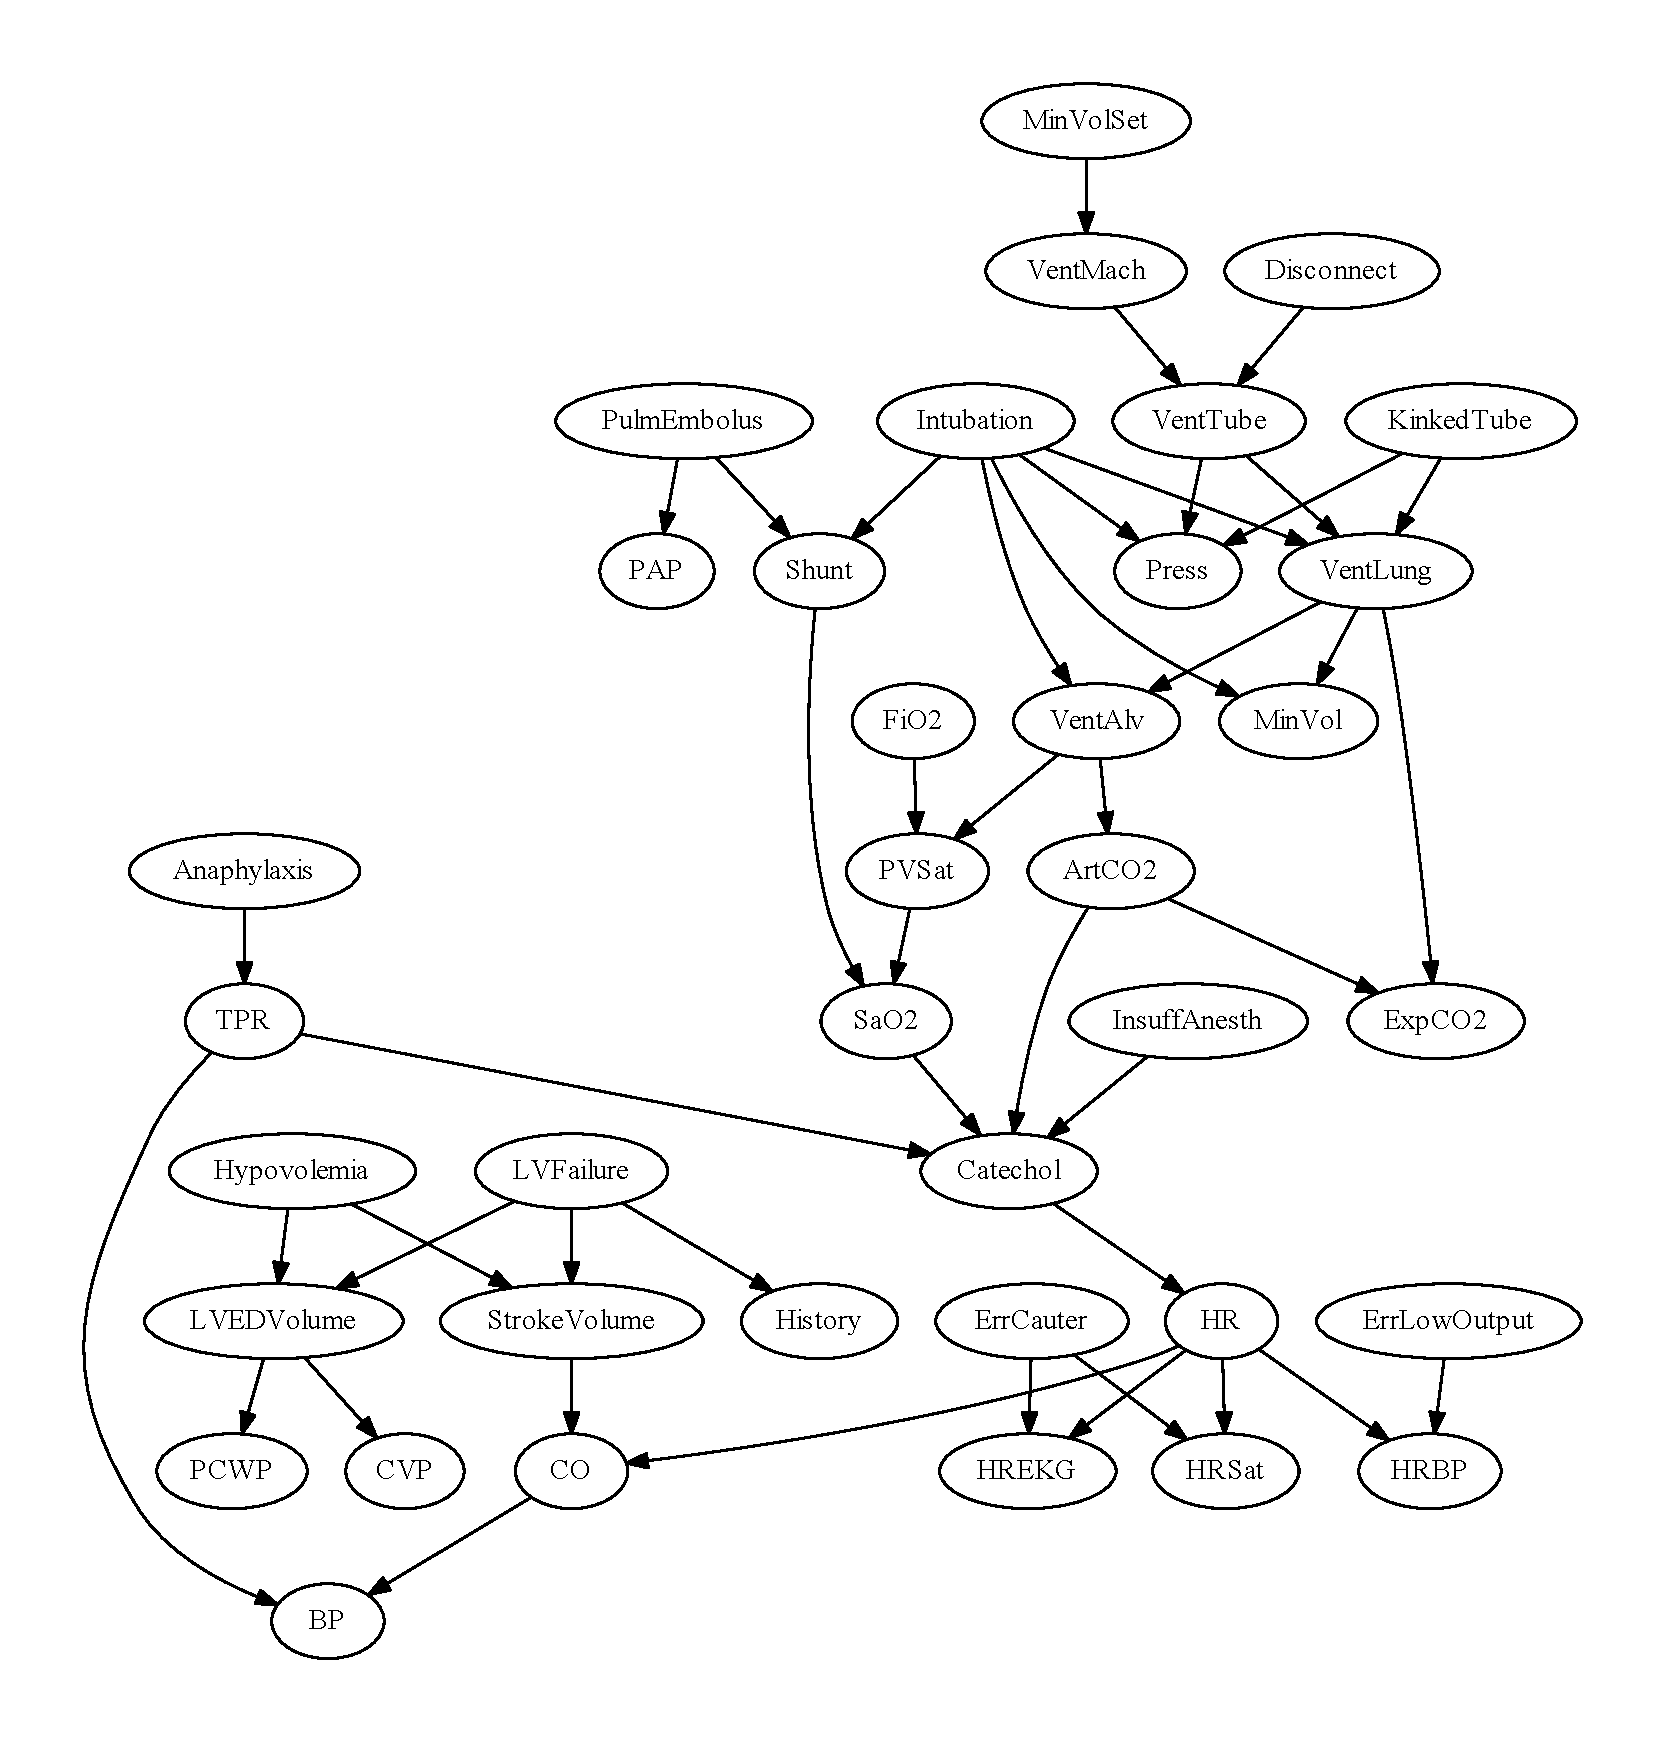
\includegraphics[scale=0.6]{alarm_reference_net.pdf}
%   \caption{ Структура байесовой сети ALARM }
%   \label{fig:arch_and_mod:asia_and_alarm:alarm_structure}
% \end{figure}


% \subsection{Алгоритм на основе оценки апостериорной вероятности структуры}
% \label{sub:arch_and_mod:k2_algorithm}

% В данном подразделе рассматривается известный алгоритм, использующий оценку апостериорной вероятности в качестве критерия поиска.
% Подробное описание данной оценки и базового алгоритма поиска приведены в работе~\cite{Cooper1991}.

% Формулу~(\ref{eq:domain:k2:model_and_data_prob}) для оценки совместной вероятности на практике напрямую использовать не получится, без введения дополнительных предположений.
% Необходимо сделать предположение, что все возможные структуры равновероятны, т.\,е. $P(B_S)$ равно некоторой малой константе $c$.
% Таким образом нахождение оптимальной структуры сводится к максимизации формулы~(\ref{eq:arch_and_mod:k2_algorithm:optimization_objective}), т.\,e. задача сводится к нахождению множества вершин"=предков $ \pi_i $ для каждой вершины $X_i$, оптимизирующих целевую функцию~\cite{Cooper1991}.
% \begin{align}
%   \label{eq:arch_and_mod:k2_algorithm:optimization_objective}
%   \max \left[ P(B_S, x^R[n]) \right] = \notag\\
%   =
%     c \prod_{i = 1}^{R} \max_{\pi_i}
%     \bigg[
%       \prod_{j = 1}^{q_i} &% to align formula
%       \frac{(\alpha_i - 1)!}
%            {(n[\phi_i[j], i, B_S] + \alpha_i - 1)!}
%       \prod_{k = 1}^{\alpha_i}
%         n[v_{ik}, \phi_i[j], i, B_S]!
%     \bigg] \text{\,.}
% \end{align}

% Таким образом наивный алгоритм поиска состоит в полном переборе всех возможных родителей для каждой вершины и оптимизации при этом функции~(\ref{eq:arch_and_mod:k2_algorithm:node_optimization_obj}):
% \begin{equation}
%   \label{eq:arch_and_mod:k2_algorithm:node_optimization_obj}
%   g(i, \pi_i) =
%     \prod_{j = 1}^{q_i}
%       \frac{(\alpha_i - 1)!}
%            {(n[\phi_i[j], i, B_S] + \alpha_i - 1)!}
%       \prod_{k = 1}^{\alpha_i}
%         n[v_{ik}, \phi_i[j], i, B_S]! \text{\,.}
% \end{equation}

% На практике наивный вариант не годится из-за большого количества возможных вариантов структур сетей.
% В разработанной реализации использовались те же ограничения и стратегия поиска, что и в работе~\cite{Cooper1991}.
% Перед началом выполнения алгоритма требуется знание о порядке вершин, таком, что вершины родители всегда находятся раньше вершин потомков.
% Схематически алгоритм поиска выглядит следующим образом:

% \begin{lstlisting}[mathescape,escapeinside={/*@}{@*/},caption={Псевдокод реализации алгоритма К2}, label=lst:arch_and_mod:k2_algorithm:k2_pseudo]
% function k2 =
%   (* Input: dataset $x^R[n]$, ordering of variables, u - maximum number of parents per variable.
%      Output: for each node, a printout of the parents of the node. *)
%   for i in 1 .. R do
%     $ \pi_i $ := $ \emptyset $
%     $P_{old}$ := $g(i, \pi_i)$; // formula(/*@\ref{eq:arch_and_mod:k2_algorithm:node_optimization_obj}@*/)
%     OkToContinue := true;
%     while OkToContinue and $|\pi_i| < u$ do
%       let z = node in $ \text{Pred}(X_i) - \pi_i $ that maximizes $ g(i, \pi_i \cup {z}) $
%       $P_{new}$ := $f(i, \pi_i \cup {z})$
%       if $P_{new} > P_{old}$ then
%         $P_{old}$ := $P_{new}$;
%         $ \pi_i $ := $ \pi_i \cup {z} $
%       else OkToContinue := false
%     end while
%     printfn("Node: ", $X_i$, "Parents of $X_i$:", $\pi_i$)
%   end for
% end
% \end{lstlisting}

% В разработанной в рамках дипломного проекта реализации за основу был взят алгоритм К2, приведенный в работе~\cite{Cooper1991}, псевдокод которого показан в листинге~\ref{lst:arch_and_mod:k2_algorithm:k2_pseudo}.
% В разработанном алгоритме слегка изменен способ подсчета целевой функции.
% Приняв во внимание ограничение на представление в компьютере вещественных и больших целых чисел, а также то, что операции умножения, деления и возведения в степень более сложные, было принято решение воспользоваться прологарифмированной версией формулы~(\ref{eq:arch_and_mod:k2_algorithm:node_optimization_obj}).
% Ниже приводится точная формула~(\ref{eq:arch_and_mod:k2_algorithm:log_node_optimization_obj}), по которой вычисляется оценка в реализованном алгоритме.
% Данная формула более удобная для вычисления на компьютере:

% \begin{align}
%   \label{eq:arch_and_mod:k2_algorithm:log_node_optimization_obj}
%   \log(g(i, \pi_i)) &=
%     \sum_{j = 1}^{q_i}
%       \log
%       \left(
%         \frac{(\alpha_i - 1)!}
%              {(n_{ij} + \alpha_{i} - 1)!}
%         \prod_{k = 1}^{\alpha_i}
%           n_{ijk}!
%       \right) =\notag\\
%     &=
%     \sum_{j = 1}^{q_i}
%       \left(
%         \log
%           \frac{(\alpha_i - 1)!}
%                {(n_{ij} + \alpha_{i} - 1)!}
%         +
%         \log
%           \prod_{k = 1}^{\alpha_i}
%             n_{ijk}!
%       \right) =\notag\\
%     &=
%     \sum_{j = 1}^{q_i}
%       \left(
%         \log (\alpha_i - 1)! - \log (n_{ij} + \alpha_{i} - 1)!
%         +
%         \sum_{k = 1}^{\alpha_i}
%           \log n_{ijk}!
%       \right) =\notag\\
%     &=
%       \sum_{j = 1}^{q_i}
%       \left(
%         \log \Gamma(\alpha_i) - \log \Gamma(n_{ij} + \alpha_{i})
%         +
%         \sum_{k = 1}^{\alpha_i}
%           \log \Gamma(n_{ijk} + 1)
%       \right) = \notag\\
%     &=
%       q_i \log \Gamma(\alpha_i) +
%       \sum_{j = 1}^{q_i}
%       \left(
%         \sum_{k = 1}^{\alpha_i}
%           \log \Gamma(n_{ijk} + 1)
%         - \log \Gamma(n_{ij} + \alpha_{i})
%       \right) \text{\,,}
% \end{align}
% \begin{explanation}
% где & $ \Gamma $ & гамма-функция "---  расширение понятия факториала на поле комплексных чисел; \\
%     & $ n_{ijk} $ & условное, более краткое, обозначение для $n[v_{ik}, \phi_i[j], i, B_S]$; \\
%     & $ n_{ij} $ & условное, более краткое, обозначение для $n[\phi_i[j], i, B_S]$.
% \end{explanation}

% Помимо использования формулы~(\ref{eq:arch_and_mod:k2_algorithm:log_node_optimization_obj}) в реализации были произведены дополнительные оптимизации, продиктованные результатами профилирования реализации алгоритма.

% Результаты обучения сетей Asia и ALARM на наборах данных разного объёма реализованным алгоритмом приведены в таблицах~\ref{table:arch_and_mod:k2_algorithm:result_asia} и~\ref{table:arch_and_mod:k2_algorithm:result_alarm} соответственно\footnote{Формат времени в колонке <<Время построения>> "--- часы:минуты:секунды.милисекунды}.
% Как видно из результатов, с увеличением количества данных улучшается качество извлеченной из данных сети.
% Стоит обратить внимание, что данный алгоритм потребовал априорных знаний о распределении, по которому были сгенерированы данные.
% Алгоритму на вход необходим определенный порядок вершин и знание максимального количества переменных"=родителей для каждой переменной.

% \begin{table}[ht]
% \caption{Качество структуры извлеченной из данных для сети Asia алгоритмом К2 из разработанной библиотеки}
% \label{table:arch_and_mod:k2_algorithm:result_asia}
%   \centering
%   \begin{tabular}{| >{\raggedleft}m{0.14\textwidth}
%                   | >{\centering}m{0.15\textwidth}
%                   | >{\centering}m{0.15\textwidth}
%                   | >{\centering}m{0.195\textwidth}
%                   | >{\centering\arraybackslash}m{0.23\textwidth}|}
%     \hline
%     \multirow{2}{0.14\textwidth}{\centering Размер данных} &
%     \multicolumn{3}{c|}{\centering Соединения} &
%     \multirow{2}{0.22\textwidth}{\centering Время построения} \\
%     \cline{2-4}
%     & пропущено & добавлено & инвертировано & \\
%     \hline
%      \num{1000} & \num{1} & \num{1} & \num{0} & 00:00:00.01 \\
%     \hline
%      \num{2000} & \num{1} & \num{1} & \num{0} & 00:00:00.02 \\
%     \hline
%      \num{4000} & \num{1} & \num{0} & \num{0} & 00:00:00.04 \\
%     \hline
%      \num{8000} & \num{1} & \num{1} & \num{0} & 00:00:00.09 \\
%     \hline
%      \num{16000} & \num{0} & \num{0} & \num{0} & 00:00:00.17 \\
%     \hline
%      \num{32000} & \num{0} & \num{0} & \num{0} & 00:00:00.36 \\
%     \hline
%      \num{64000} & \num{0} & \num{0} & \num{0} & 00:00:00.80 \\
%     \hline
%      \num{1048576} & \num{0} & \num{0} & \num{0} & 00:00:11.41 \\
%     \hline
%   \end{tabular}
% \end{table}

% \begin{table}[ht]
% \caption{Качество структуры извлеченной из данных для сети ALARM алгоритмом К2 из разработанной библиотеки}
% \label{table:arch_and_mod:k2_algorithm:result_alarm}
%   \centering
%   \begin{tabular}{| >{\raggedleft}m{0.14\textwidth}
%                   | >{\centering}m{0.15\textwidth}
%                   | >{\centering}m{0.15\textwidth}
%                   | >{\centering}m{0.195\textwidth}
%                   | >{\centering\arraybackslash}m{0.23\textwidth}|}
%     \hline
%     \multirow{2}{0.14\textwidth}{\centering Размер данных} &
%     \multicolumn{3}{c|}{\centering Соединения} &
%     \multirow{2}{0.22\textwidth}{\centering Время построения} \\
%     \cline{2-4}
%     & пропущено & добавлено & инвертировано & \\
%     \hline
%      \num{1000} & \num{1} & \num{5} & \num{0} & 00:00:00.75 \\
%     \hline
%      \num{2000} & \num{1} & \num{1} & \num{0} & 00:00:00.72 \\
%     \hline
%      \num{4000} & \num{1} & \num{0} & \num{0} & 00:00:01.29 \\
%     \hline
%      \num{8000} & \num{1} & \num{2} & \num{0} & 00:00:02.45 \\
%     \hline
%      \num{16000} & \num{0} & \num{2} & \num{0} & 00:00:04.83 \\
%     \hline
%      \num{32000} & \num{0} & \num{1} & \num{0} & 00:00:09.48 \\
%     \hline
%      \num{64000} & \num{0} & \num{1} & \num{0} & 00:00:18.61 \\
%     \hline
%      \num{128000} & \num{0} & \num{1} & \num{0} & 00:00:36.58 \\
%     \hline
%      \num{1048576} & \num{0} & \num{1} & \num{0} & 00:04:57.18 \\
%     \hline
%      \num{8388608} & \num{0} & \num{1} & \num{0} & 00:44:13.00 \\
%     \hline
%   \end{tabular}
% \end{table}

% Произведём сравнение реализованного алгоритма, с аналогичным алгоритмом реализованным в программе GeNIe, описанной в пункте~\ref{sub:domain:existing_programs:genie} на странице~\pageref{sub:domain:existing_programs:genie}.
% В таблице~\ref{table:arch_and_mod:k2_algorithm:genie_asia_k2} приводятся полученные результаты.

% \begin{table}[ht]
% \caption{Качество структуры извлеченной из данных для сети Asia программой GeNIe с применением алгоритма Greedy Thick Thinning с оценкой K2}
% \label{table:arch_and_mod:k2_algorithm:genie_asia_k2}
%   \centering
%   \begin{tabular}{| >{\raggedleft}m{0.14\textwidth}
%                   | >{\centering}m{0.15\textwidth}
%                   | >{\centering}m{0.15\textwidth}
%                   | >{\centering}m{0.195\textwidth}
%                   | >{\centering\arraybackslash}m{0.23\textwidth}|}
%     \hline
%     \multirow{2}{0.14\textwidth}{\centering Размер данных} &
%     \multicolumn{3}{c|}{\centering Соединения} &
%     \multirow{2}{0.22\textwidth}{\centering Время построения} \\
%     \cline{2-4}
%     & пропущено & добавлено & инвертировано & \\
%     \hline
%      \num{1000} & \num{2} & \num{2} & \num{2} & \emph{не измерялось} \\
%     \hline
%      \num{2000} & \num{2} & \num{3} & \num{2} & \emph{не измерялось} \\
%     \hline
%      \num{4000} & \num{1} & \num{1} & \num{3} & \emph{не измерялось} \\
%     \hline
%      \num{8000} & \num{2} & \num{4} & \num{2} & \emph{не измерялось} \\
%     \hline
%      \num{16000} & \num{2} & \num{5} & \num{2} & \emph{не измерялось} \\
%     \hline
%      \num{32000} & \num{1} & \num{4} & \num{2} & \emph{не измерялось} \\
%     \hline
%      \num{64000} & \num{0} & \num{1} & \num{3} & \emph{не измерялось} \\
%     \hline
%      \num{1048576} & \num{1} & \num{4} & \num{2} & \emph{не измерялось} \\
%     \hline
%   \end{tabular}
% \end{table}

% Для сравнения реализованных в библиотеке алгоритмов с теми, которые есть в GeNIe, были произведены дополнительные испытания последних.
% Для наиболее <<точного>> алгоритма реализованного в GeNIe в таблице~\ref{table:arch_and_mod:k2_algorithm:genie_asia_pc} приводится оценка качества полученной структуры на наборах данных различного размера
% Для трех других алгоритмов в таблице~\ref{table:arch_and_mod:k2_algorithm:genie_asia_other} "--- на самом большом наборе данных.
% Как видно из полученных экспериментально данных, реализация алгоритма на основе оценки апостериорной вероятности из разработанной библиотеки ведет себя лучше как на малых объёмах данных, так и на больших, не смотря на то, что некоторые алгоритмы реализованные в GeNIe используют тот же метод оценки.

% \begin{table}[ht]
% \caption{Качество структуры извлеченной из данных для сети Asia программой GeNIe с использованием алгоритма PC}
% \label{table:arch_and_mod:k2_algorithm:genie_asia_pc}
%   \centering
%   \begin{tabular}{| >{\raggedleft}m{0.14\textwidth}
%                   | >{\centering}m{0.15\textwidth}
%                   | >{\centering}m{0.15\textwidth}
%                   | >{\centering}m{0.195\textwidth}
%                   | >{\centering\arraybackslash}m{0.23\textwidth}|}
%     \hline
%     \multirow{2}{0.14\textwidth}{\centering Размер данных} &
%     \multicolumn{3}{c|}{\centering Соединения} &
%     \multirow{2}{0.22\textwidth}{\centering Время построения} \\
%     \cline{2-4}
%     & пропущено & добавлено & инвертировано & \\
%     \hline
%      \num{1000} & \num{2} & \num{1} & \num{2} & \emph{не измерялось} \\
%     \hline
%      \num{2000} & \num{3} & \num{0} & \num{0} & \emph{не измерялось} \\
%     \hline
%      \num{4000} & \num{1} & \num{0} & \num{0} & \emph{не измерялось} \\
%     \hline
%      \num{8000} & \num{2} & \num{0} & \num{0} & \emph{не измерялось} \\
%     \hline
%      \num{16000} & \num{3} & \num{1} & \num{3} & \emph{не измерялось} \\
%     \hline
%      \num{32000} & \num{2} & \num{0} & \num{0} & \emph{не измерялось} \\
%     \hline
%      \num{64000} & \num{1} & \num{0} & \num{0} & \emph{не измерялось} \\
%     \hline
%      \num{1048576} & \num{1} & \num{0} & \num{0} & \emph{не измерялось} \\
%     \hline
%   \end{tabular}
% \end{table}

% \begin{table}[ht]
% \caption{Качество структуры извлеченной из данных для сети Asia программой GeNIe на наборе данных из \num{1048576} случаев}
%   \label{table:arch_and_mod:k2_algorithm:genie_asia_other}
%   \centering
%   \begin{tabular}{| >{\raggedright}m{0.405\textwidth}
%                   | >{\centering}m{0.15\textwidth}
%                   | >{\centering}m{0.14\textwidth}
%                   | >{\centering\arraybackslash}m{0.195\textwidth}|}
%     \hline
%     \multirow{2}{0.37\textwidth}{\centering Алгоритм} &
%     \multicolumn{3}{c|}{\centering Соединения}  \\
%     \cline{2-4}
%     & пропущено & добавлено & инвертировано \\
%     \hline
%      Bayesian Search & \num{0} & \num{2} & \num{5} \\
%     \hline
%      Essential Graph Search & \num{5} & \num{0} & \num{2} \\
%     \hline
%      Greedy Thick Thinning с оценкой BDeu & \num{1} & \num{4} & \num{2} \\
%     \hline
%   \end{tabular}
% \end{table}


% \subsection{Алгоритм на основе оценки минимальной длины описания}
% \label{sub:arch_and_mod:mdl_algorithm1}
% Помимо алгоритма использующего оценку апостериорной вероятности в разработанной библиотеке был реализован алгоритм использующий оценку на основе принципа МДО.
% Описание принципа МДО приведено в подразделе~\ref{sub:domain:mdl_principle} данной пояснительной записки.
% Т.\,к. способ подсчета оценки уже был здесь описан, то необходимо привести описание процедуры поиска.
% Процедура поиска в разработанной реализации алгоритма поиска вдохновлена процедурой поиска, использованной в работе~\cite{terentyev_2006}.

% Данный алгоритм нахождения структуры не требует предварительных знаний об истинном распределении, в отличие от алгоритма описанного в подразделе~\ref{sub:arch_and_mod:k2_algorithm}, что является существенным преимуществом на практике.
% Вместо использования априорных знаний, реализация алгоритма используем предварительные вычисления, извлекающие полезные данные о взаимозависимостях между переменным.
% Затем эта информация используется в стратегии поиска структуры.

% В качестве оценки степени зависимости двух произвольных переменных в работе~\cite{Chow68approximatingdiscrete} было предложено использовать значение взаимной информации\footnote{В англоязычной литературе используется термин mutual information}.
% Эта информация задаёт приоритет поиска зависимостей между переменными.
% По своей сути значение обоюдной информации является аналогом корреляции, но по своему содержанию "--- это оценка количества информации содержащейся в одной переменной о другой~\cite{terentyev_2006}.
% Значение взаимной информации принимает неотрицательные значения и равно нулю в случае независимости случайных величин.
% Для вычисления взаимной информации была предложена формула~(\ref{eq:arch_and_mod:mdl_algorithm1:mutual_information}):
% \begin{equation}
%   \label{eq:arch_and_mod:mdl_algorithm1:mutual_information}
%   I(X; Y) = \sum_{y \in Y} \sum_{x \in X}
%                  p(x, y) \log{ \left(\frac{p(x, y)}{p(x)\,p(y)}
%                               \right) } \text{\,,}
% \end{equation}
% \begin{explanation}
% где & $ p(x, y)$ & совместное распределение случайных величин $X$ и $Y$; \\
%     & $ p(y) $ & безусловное распределение случайной величины $X$; \\
%     & $ p(x) $ & безусловное распределение случайной величины $Y$.
% \end{explanation}

% На практике при вычислении $I(X; Y)$ следует соблюдать осторожность, т.\,к. относительные частоты, используемые для оценки $p(x)$, $p(y)$ и $p(x, y)$, могут необоснованно принимать значение \num{0} из-за отсутствия некоторых состояний переменных в наблюдаемых данных.
% В таких случаях вместо нуля используется достаточно малое число.

% Таким образом алгоритм поиска состоит из следующих шагов:
% \begin{enumerate}
%   \item Вычислить значения взаимной информации между всеми парами переменных и отсортировать список уникальных пар по убыванию взаимной информации.
%   Пусть данный список обозначается символом $list$.
%   \item Алгоритм поиска начинается с извлечения двух пар переменных $(X_{i1}, X_{i2})$ и $(X_{j1}, X_{j2})$ из списка $list$ с максимальным значением взаимной информации.
%   Затем среди всех возможных ацикличных моделей, построенных из переменных $ X_{i1}, X_{i2}, X_{j1}, X_{j2} $ выбирается модель с наименьшей оценкой, вычисленной по формуле~(\ref{eq:domain:mdl:description_length}).
%   Эта модель принимается за стартовую модель $g_0$
%   \item Пока список $list$ не пуст из него извлекается пара переменных $(X_{k1}, X_{k2})$ и строится множество новых моделей $\{g_0; g_0 \cup (X_{k1}, X_{k2}); g_0 \cup (X_{k2}, X_{k1})\} $.
%   И этого множества удаляются циклические модели и выбирается модель с минимальной оценкой по формуле~(\ref{eq:domain:mdl:description_length}) и присваивается переменной $g_0$.
%   \item Когда список $list$ пуст, то поиск прекращается, модель $g_0$ считается оптимальной и рассматривается как структура вероятностной сети выведенная из данных.
%   На практике можно завершить алгоритм раньше не дожидаясь пустоты $list$.
% \end{enumerate}

% При реализации данного алгоритма важным моментом для повышения производительности является мемоизация значений функций $n[s, k, g]$ и $n[q, s, k, g]$, т.\,к. оценка длины описания считается для всей модели сразу, но между двумя последовательными итерациями разница между моделями составляем максимум одно соединение, т.\,е. для большинства вершин множество предков не меняется и значения $n[s, k, g]$ и $n[q, s, k, g]$ остаются неизменными и их можно не вычислять каждый раз.
% Так, для сети ALARM на экспериментальных данных из \num{1048576} случаев, время построения сети сократилось с более чем четырех часов, до двух с половиной минут.
% Ниже приведены результаты качества обучения данного алгоритма для сети Asia, в табилце~\ref{table:arch_and_mod:mdl_algorithm1:asia_mdl}, и для сети ALARM, в таблице~\ref{table:arch_and_mod:mdl_algorithm1:alarm_mdl}.

% \begin{table}[ht]
% \caption{Качество структуры извлеченной из данных для сети Asia алгоритмом из разработанной библиотеки, использующим оценку МДО}
% \label{table:arch_and_mod:mdl_algorithm1:asia_mdl}
%   \centering
%   \begin{tabular}{| >{\raggedleft}m{0.14\textwidth}
%                   | >{\centering}m{0.15\textwidth}
%                   | >{\centering}m{0.15\textwidth}
%                   | >{\centering}m{0.195\textwidth}
%                   | >{\centering\arraybackslash}m{0.23\textwidth}|}
%     \hline
%     \multirow{2}{0.14\textwidth}{\centering Размер данных} &
%     \multicolumn{3}{c|}{\centering Соединения} &
%     \multirow{2}{0.22\textwidth}{\centering Время построения} \\
%     \cline{2-4}
%     & пропущено & добавлено & инвертировано & \\
%     \hline
%      \num{1000} & \num{2} & \num{1} & \num{0} & 00:00:00.26 \\
%     \hline
%      \num{2000} & \num{2} & \num{2} & \num{2} & 00:00:00.28 \\
%     \hline
%      \num{4000} & \num{1} & \num{2} & \num{2} & 00:00:00.47 \\
%     \hline
%      \num{8000} & \num{1} & \num{1} & \num{0} & 00:00:00.93 \\
%     \hline
%      \num{16000} & \num{1} & \num{2} & \num{0} & 00:00:01.70 \\
%     \hline
%      \num{32000} & \num{0} & \num{1} & \num{1} & 00:00:03.37 \\
%     \hline
%      \num{64000} & \num{0} & \num{1} & \num{0} & 00:00:07.05 \\
%     \hline
%      \num{1048576} & \num{0} & \num{1} & \num{0} & 00:01:46.53 \\
%     \hline
%   \end{tabular}
% \end{table}

% \begin{table}[ht]
% \caption{Качество структуры извлеченной из данных для сети ALARM алгоритмом из разработанной библиотеки, использующим оценку МДО}
% \label{table:arch_and_mod:mdl_algorithm1:alarm_mdl}
%   \centering
%   \begin{tabular}{| >{\raggedleft}m{0.14\textwidth}
%                   | >{\centering}m{0.15\textwidth}
%                   | >{\centering}m{0.15\textwidth}
%                   | >{\centering}m{0.195\textwidth}
%                   | >{\centering\arraybackslash}m{0.23\textwidth}|}
%     \hline
%     \multirow{2}{0.14\textwidth}{\centering Размер данных} &
%     \multicolumn{3}{c|}{\centering Соединения} &
%     \multirow{2}{0.22\textwidth}{\centering Время построения} \\
%     \cline{2-4}
%     & пропущено & добавлено & инвертировано & \\
%     \hline
%      \num{1000} & \num{6} & \num{3} & \num{11} & 00:00:01.78 \\
%     \hline
%      \num{2000} & \num{5} & \num{5} & \num{11} & 00:00:01.50 \\
%     \hline
%      \num{4000} & \num{3} & \num{4} & \num{11} & 00:00:01.84 \\
%     \hline
%      \num{8000} & \num{3} & \num{7} & \num{9} & 00:00:02.26 \\
%     \hline
%      \num{16000} & \num{2} & \num{10} & \num{17} & 00:00:03.27 \\
%     \hline
%      \num{32000} & \num{2} & \num{13} & \num{19} & 00:00:05.17 \\
%     \hline
%      \num{64000} & \num{1} & \num{17} & \num{15} & 00:00:09.30 \\
%     \hline
%      \num{128000} & \num{1} & \num{21} & \num{21} & 00:00:18.50 \\
%     \hline
%      \num{1048576} & \num{0} & \num{22} & \num{16} & 00:02:22.82 \\
%     \hline
%   \end{tabular}
% \end{table}

% Как видно данный алгоритм работает хуже алгоритма из подраздела~\ref{sub:arch_and_mod:k2_algorithm}.
% По результатам измерений, приведенных в табилце~\ref{table:arch_and_mod:mdl_algorithm1:alarm_mdl} можно видеть, что с увеличением набора данных структура сети усложняется.
% Количество пропущенных связей уменьшается, но также растет количество лишних и инвертированных связей.
% На практике возможна доработка структуры сети с участием эксперта.
% Это займет меньше времени, чем разработка сети <<с нуля>>, т.\,к. большинство связей и общая структура уже найдены.
% В защиту данного алгоритма можно сказать, что он работает без каких-либо априорных знаний о структуре сети и не ограничен максимальным количеством вершин"=предков, как алгоритм из предыдущего подраздела.
% Также можно заметить, что не смотря на то, что алгоритм проигрывает реализации алгоритма K2, качество обучаемой структуры в многих случаях лучше того, что может предоставить программа GeNIe.
% Сравнение с различными алгоритмами GeNIe приведено в таблице~\ref{table:arch_and_mod:mdl_algorithm1:genie_alarm_other}, необходимо отметить, что алгоритмы из GeNIe субъективно работают в разы медленнее разработанной библиотеки на данных из \num{1048576} случаев для сети ALARM.
% Например, выполнение алгоритма Bayesian Search заняло более четырёх часов.

% \begin{table}[ht]
% \caption{Качество структуры извлеченной из данных для сети ALARM программой GeNIe на наборе данных из \num{1048576} случаев}
%   \label{table:arch_and_mod:mdl_algorithm1:genie_alarm_other}
%   \centering
%   \begin{tabular}{| >{\raggedright}m{0.405\textwidth}
%                   | >{\centering}m{0.15\textwidth}
%                   | >{\centering}m{0.14\textwidth}
%                   | >{\centering\arraybackslash}m{0.195\textwidth}|}
%     \hline
%     \multirow{2}{0.37\textwidth}{\centering Алгоритм} &
%     \multicolumn{3}{c|}{\centering Соединения}  \\
%     \cline{2-4}
%     & пропущено & добавлено & инвертировано \\
%     \hline
%      Bayesian Search & \num{8} & \num{66} & \num{21} \\
%     \hline
%      PC & \multicolumn{3}{c|}{\centering создал циклическую структуру} \\
%     \hline
%      Essential Graph Search & \num{32} & \num{2} & \num{4} \\
%     \hline
%      Greedy Thick Thinning с оценкой BDeu & \num{0} & \num{26} & \num{24} \\
%     \hline
%      Greedy Thick Thinning с оценкой K2 & \num{0} & \num{30} & \num{23} \\
%     \hline
%   \end{tabular}
% \end{table}

% В процессе оценки результатов данного алгоритма было выявлено экспериментальным путём, что оценка на основе МДО довольная чувствительна к данным, т.\,е. имея два набора данных одинакового размера, сгенерированных одним распределением, можно получить немного разные сети из-за случайных различий в данных.
% В связи с этим была проделана следующая модификация в существующем алгоритме, которая позволила получать улучшенные сети на малых объёмах данных.
% Когда на вход алгоритму подается набор данных из $n$ случаев, то алгоритм случайным образом отбрасывает из него небольшой процент данных и строит структуру сети на уменьшенном объёме данных.
% Далее указанная операция повторяется некоторое количество раз.
% В итоге получается некоторое множество сетей из которых выбирается лучшая, используя оценку МДО и исходный набор экспериментальных данных.
% Результаты работы модифицированного алгоритма приведены в таблицах~\ref{table:arch_and_mod:mdl_algorithm1:asia_mdl_mod} и~\ref{table:arch_and_mod:mdl_algorithm1:alarm_mdl_mod}.
% Как видно из результатов, в некоторых случаях результаты незначительно улучшились, в некоторых "--- ухудшились.
% С учетом времени работы алгоритмов вопрос о целесообразности данной модификации остается открытым.

% \begin{table}[ht]
% \caption{Качество структуры извлеченной из данных для сети Asia модифицированным алгоритмом из разработанной библиотеки, использующим оценку МДО}
% \label{table:arch_and_mod:mdl_algorithm1:asia_mdl_mod}
%   \centering
%   \begin{tabular}{| >{\raggedleft}m{0.14\textwidth}
%                   | >{\centering}m{0.15\textwidth}
%                   | >{\centering}m{0.15\textwidth}
%                   | >{\centering}m{0.195\textwidth}
%                   | >{\centering\arraybackslash}m{0.23\textwidth}|}
%     \hline
%     \multirow{2}{0.14\textwidth}{\centering Размер данных} &
%     \multicolumn{3}{c|}{\centering Соединения} &
%     \multirow{2}{0.22\textwidth}{\centering Время построения} \\
%     \cline{2-4}
%     & пропущено & добавлено & инвертировано & \\
%     \hline
%      \num{1000} & \num{1} & \num{0} & \num{1} & 00:00:00.92 \\
%     \hline
%      \num{2000} & \num{1} & \num{0} & \num{0} & 00:00:00.36 \\
%     \hline
%      \num{4000} & \num{0} & \num{0} & \num{0} & 00:00:00.42 \\
%     \hline
%      \num{8000} & \num{0} & \num{0} & \num{1} & 00:00:00.67 \\
%     \hline
%      \num{16000} & \num{1} & \num{2} & \num{0} & 00:00:01.44 \\
%     \hline
%      \num{32000} & \num{0} & \num{1} & \num{0} & 00:00:02.25 \\
%     \hline
%      \num{64000} & \num{0} & \num{1} & \num{0} & 00:00:03.90 \\
%     \hline
%      \num{1048576} & \num{0} & \num{1} & \num{0} & 00:01:06.87 \\
%     \hline
%   \end{tabular}
% \end{table}

% \begin{table}[!ht]
% \caption{Качество структуры извлеченной из данных для сети ALARM модифицированным алгоритмом из разработанной библиотеки, использующим оценку МДО}
% \label{table:arch_and_mod:mdl_algorithm1:alarm_mdl_mod}
%   \centering
%   \begin{tabular}{| >{\raggedleft}m{0.14\textwidth}
%                   | >{\centering}m{0.15\textwidth}
%                   | >{\centering}m{0.15\textwidth}
%                   | >{\centering}m{0.195\textwidth}
%                   | >{\centering\arraybackslash}m{0.23\textwidth}|}
%     \hline
%     \multirow{2}{0.14\textwidth}{\centering Размер данных} &
%     \multicolumn{3}{c|}{\centering Соединения} &
%     \multirow{2}{0.22\textwidth}{\centering Время построения} \\
%     \cline{2-4}
%     & пропущено & добавлено & инвертировано & \\
%     \hline
%      \num{1000} & \num{7} & \num{6} & \num{10} & 00:00:11.21 \\
%     \hline
%      \num{2000} & \num{3} & \num{8} & \num{10} & 00:00:08.22 \\
%     \hline
%      \num{4000} & \num{3} & \num{8} & \num{15} & 00:00:09.89 \\
%     \hline
%      \num{8000} & \num{3} & \num{7} & \num{11} & 00:00:13.00 \\
%     \hline
%      \num{16000} & \num{1} & \num{7} & \num{15} & 00:00:18.10 \\
%     \hline
%      \num{32000} & \num{2} & \num{12} & \num{9} & 00:00:31.90 \\
%     \hline
%      \num{64000} & \num{0} & \num{8} & \num{17} & 00:00:51.33 \\
%     \hline
%      \num{128000} & \num{0} & \num{11} & \num{16} & 00:01:33.80 \\
%     \hline
%      \num{1048576} & \num{0} & \num{15} & \num{11} & 00:13:51.61 \\
%     \hline
%   \end{tabular}
% \end{table}

% Также, вероятно, стоит упомянуть что в разработанной библиотеке реализован еще один алгоритм, использующий оценку МДО, но с использованием другой стратегии поиска и другого способа вычисления длинны описания.
% Данный алгоритм и оценка были позаимствованы из работы~\cite{Lam94learningbayesian}.
% Реализация данного алгоритма проявила себя хуже, чем предыдущие два рассмотренных алгоритма и поэтому детальная информация по данному алгоритму здесь не приводится.

% В качестве промежуточного итога для данного раздела стоит отметить, что два известных алгоритма и одна модификация, реализованные в библиотеке, показывают результаты лучше как по качеству, так и по времени, чем все алгоритмы, представленные в бесплатной программе GeNIe.
% Из-за лицензионных ограничений сравнить реализованные алгоритмы с другим коммерческим ПО не удалось.

\section{Тестирование приложения}
\label{sec:testing}


\section{Методика~использования разработанного приложения}
\label{sec:usage}
Программное средство лексической и функциональной обфускации проектных описаний цифровых устройств представляет собой консольное приложение, которое может работать под управлением операционных систем семейства Windows и *nix. Корректная работа приложения гарантируется в ОС, перечисленных в разделе, описывающем анализ предметной области и укрупненную спецификацию требований. Данная методика использования программного сердства составлена с использованием операционной системы Arch Linux и симулятора терминала Sakura. Поскольку приложение является консольным и не содержит промежуточных состояний, в качестве управления используются аргументы, передаваемые при запуске приложения. Запуск приложения без аргументов(или с использованием аргументов -h или -help) и результат его работы представлены на рисунке \ref{fig:sec:usage:without_args}.

При запуске приложения в аналитическом режиме проверяется правильность кода, однако не выполняется его обфускация. Анализатор проверяет каждую сущность в дизайне и если она верна, то выводится соответствующее сообщение:

\begin{figure}[hbtp]
\centering
  
\includegraphics[scale=0.65]{analyze_success.jpg}
  \caption{ Запуск приложения в аналитическом режиме с корректным входным файлом }
  \label{fig:sec:usage:analyze_success}
\end{figure}

\afterpage{
  \begin{landscape}
  \thispagestyle{lscape}
  \begin{figure}[htbp]
  \centering
    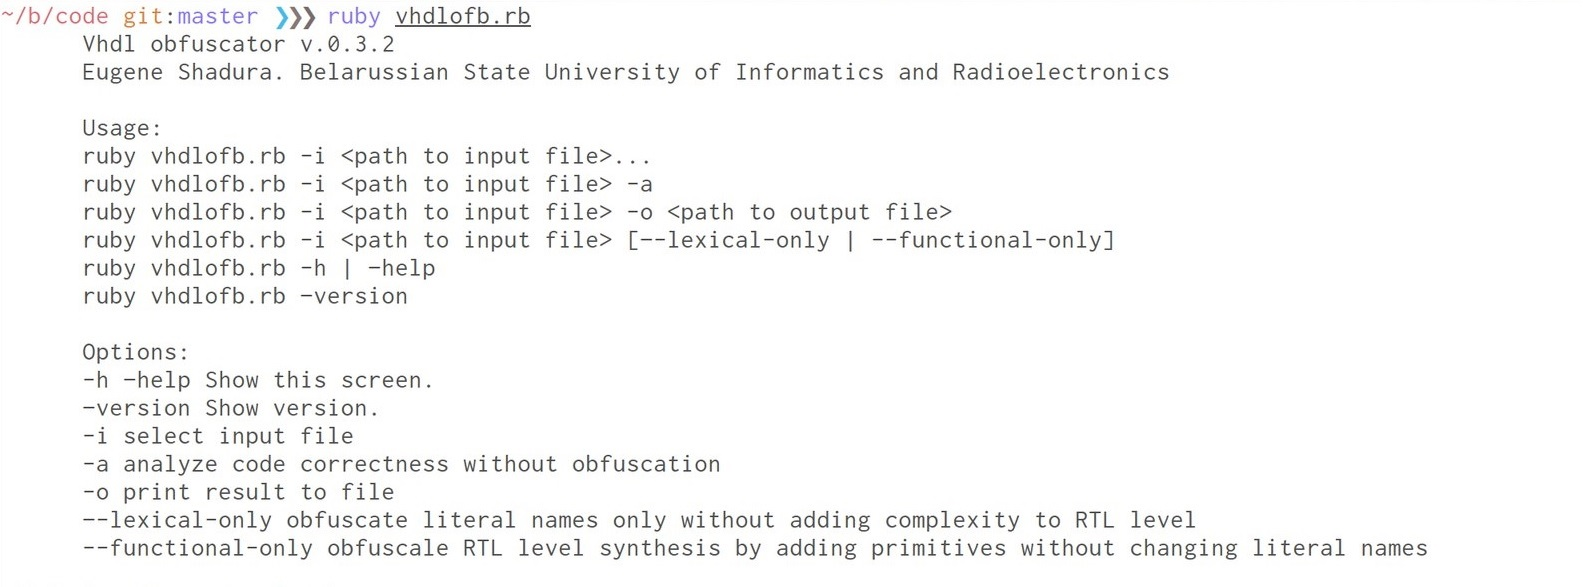
\includegraphics[scale=0.65]{without_args.jpg}
    \caption{ Запуск приложения без аргументов }
    \label{fig:sec:usage:without_args}
  \end{figure}
  \end{landscape}

}

Если же исходный код содержит какие-либо ошибки, то пользователь увидит сообщение с ошибкой, которое содержит символ, который привёл к ней:


\begin{figure}[ht]
\centering
  
\includegraphics[scale=0.65]{analyze_error.jpg}
  \caption{ Запуск приложения в аналитическом режиме с некорректным входным файлом }
  \label{fig:sec:usage:analyze_error}
\end{figure}

\begin{landscape}
\thispagestyle{lscape}
\begin{figure}[ht]
\centering
  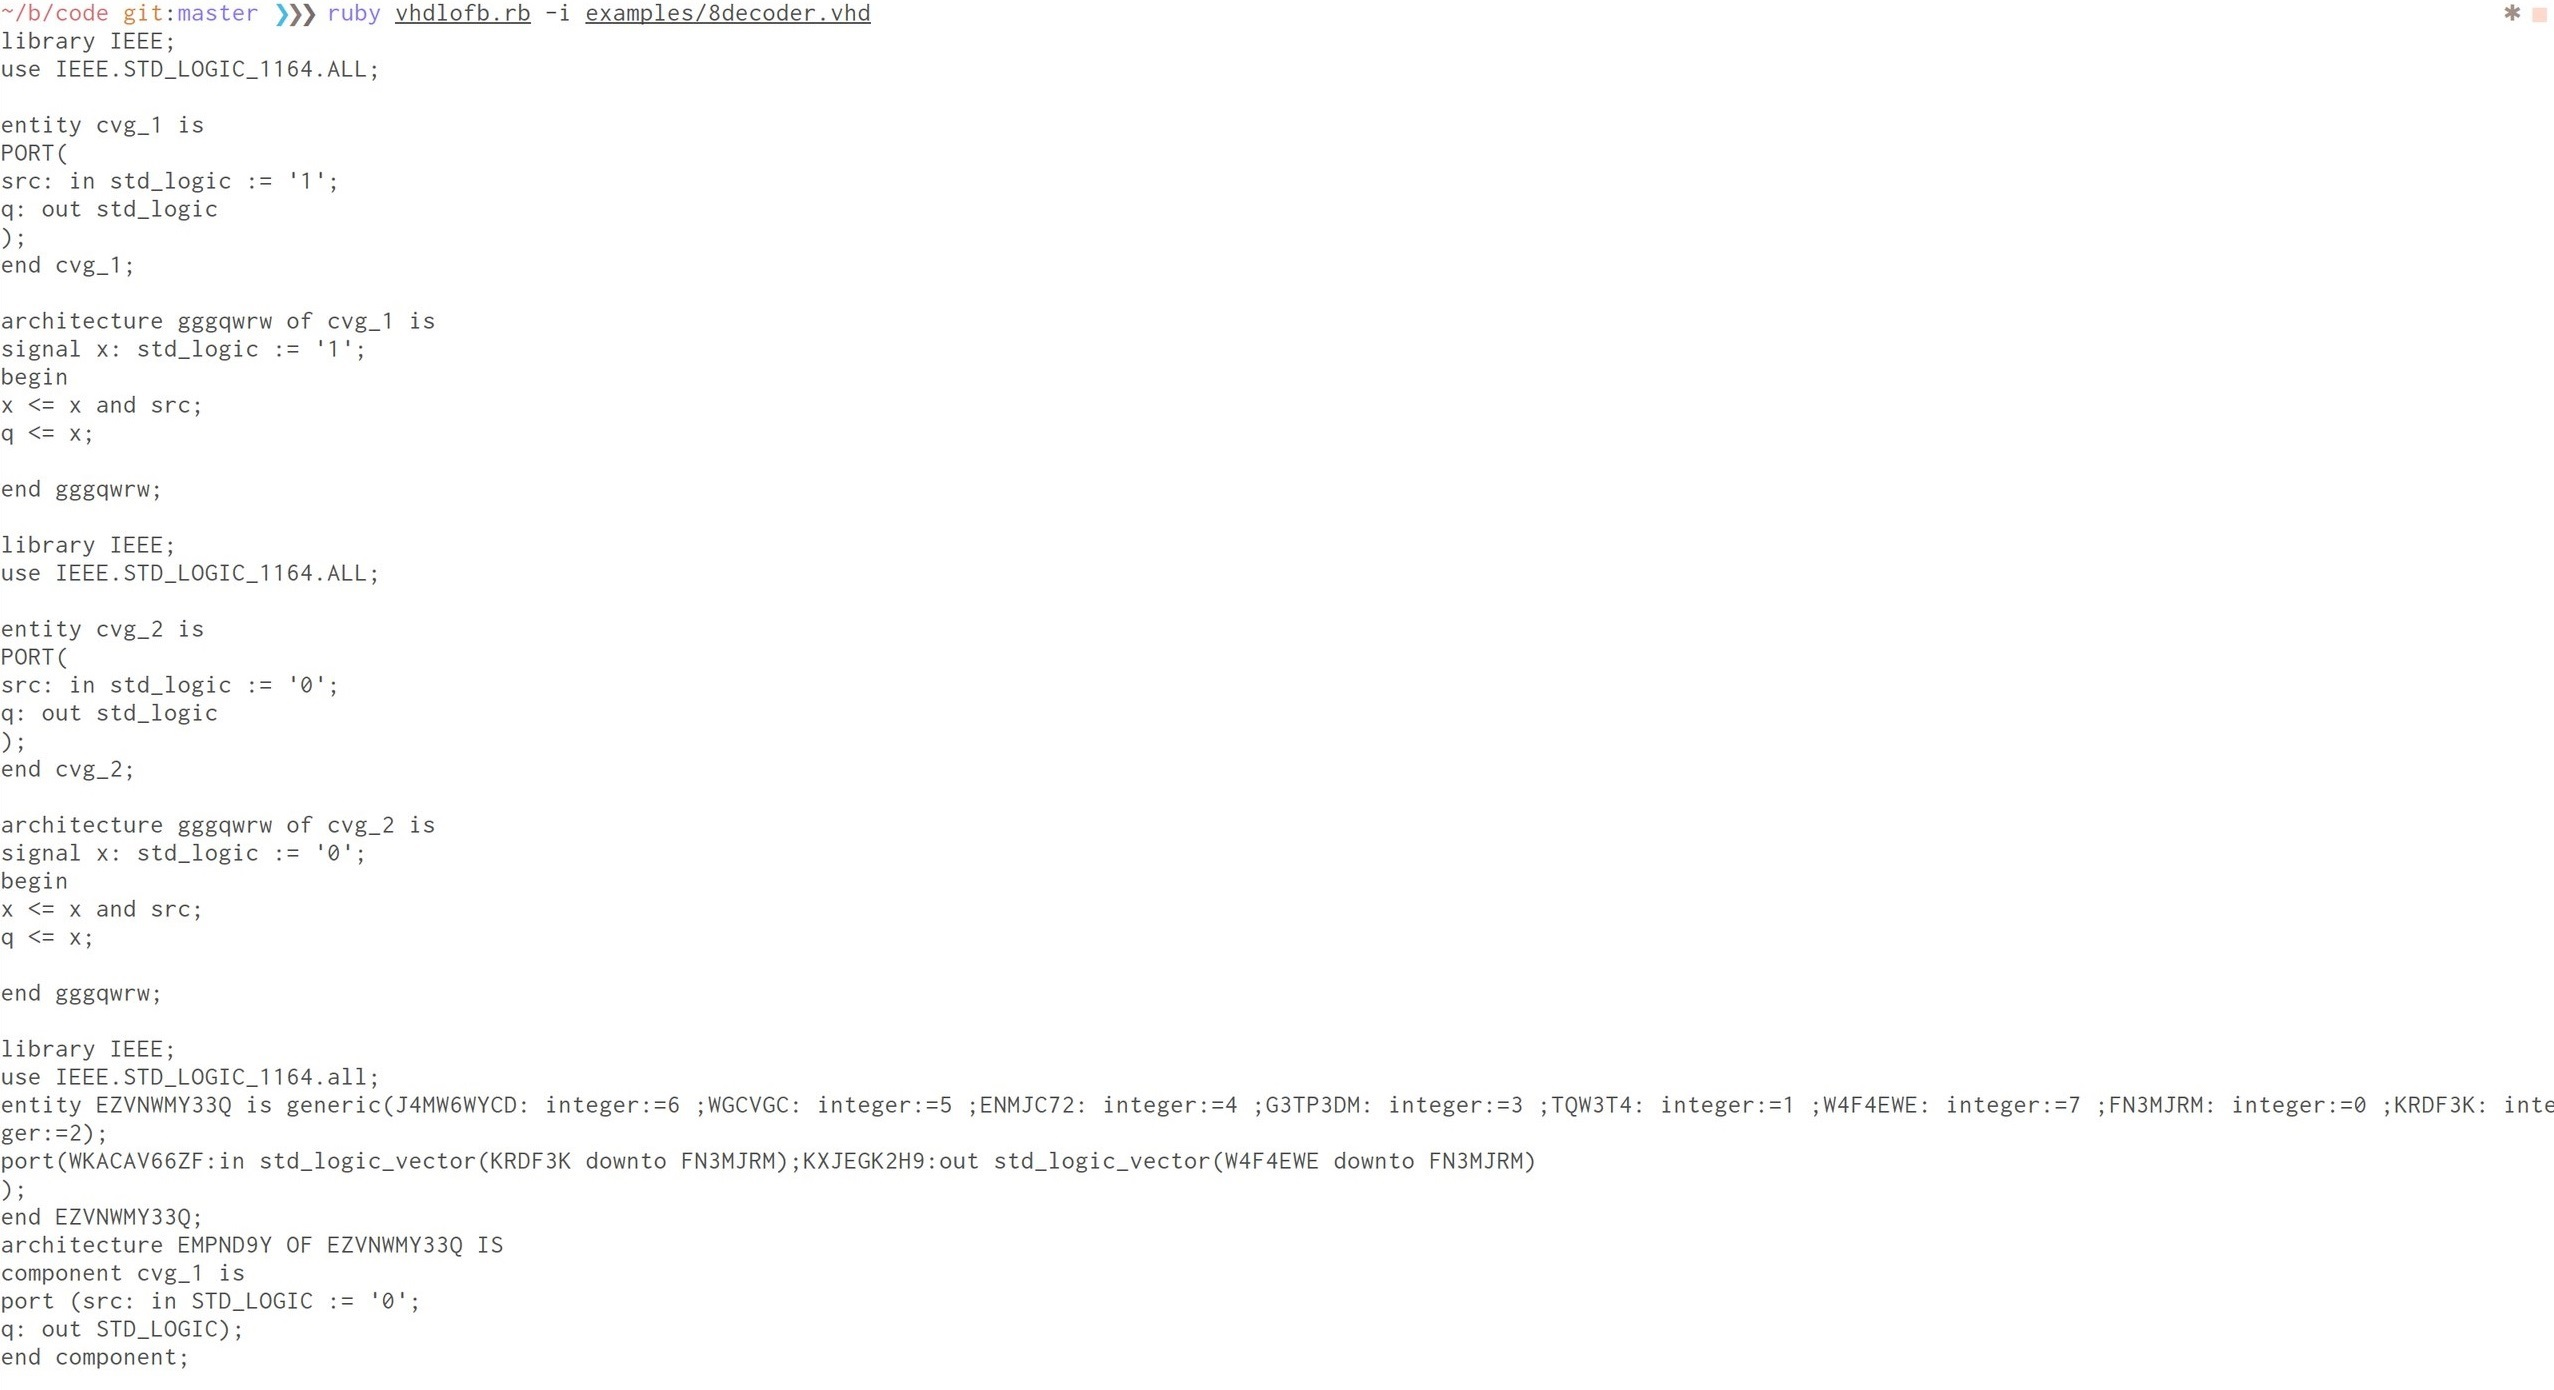
\includegraphics[scale=0.25]{without_output.jpg}
  \caption{ Запуск приложения без указания выходного файла }
  \label{fig:sec:usage:without_output}
\end{figure}
\end{landscape}

\clearpage


% \newcommand{\companyname}{\mbox{<<Техартгруп>>}}

\section{Охрана труда}

\subsection[Обеспечение пожарной безопасности на предприятии]{Обеспечение пожарной безопасности на предприятии малого бизнеса \companyname{}}


Целью дипломного проекта является реализация и анализ алгоритмов построения вероятностных сетей.
Вероятностная сеть является компактным и эффективным способом представления знаний.
Вероятностные сети используются в программном обеспечении для принятия решения в условиях недостаточной определенности.
Данный способ статистического моделирования показал свою пригодность в реальных условиях в сложных предметных областях: медицине, космической промышленности, финансовой сфере и других областях.
Первоначальные стадии разработки дипломного проекта выполнялись на предприятии ООО~\companyname{} во время прохождения преддипломной практики.
В настоящем разделе рассматриваются вопросы, связанные с обеспечением пожарной безопасности на предприятии.

Предприятие \companyname{} занимается предоставлением услуг по разработке информационных систем для иностранных предприятий. 
В минском офисе компании на данный момент работает более 200 человек. 
% TODO: Переписать абсолютный бред в оставшейся части абзаца.
Большое количество конкурирующих компаний, разрабатывающих программное обеспечение в Минске, способствует повышению общего уровня условий труда.
Это, в частности, сказывается на комфортабельности рабочих мест.
Работникам предоставляются светлые, проветриваемые, тихие кабинеты, гибкий график рабочего времени, специальные комнаты отдыха и т.\,д.
Современные компании негласно ориентируются на соответствие лучшим мировым практикам в области охраны труда и, в частности, пожарной безопасности.

На предприятии \companyname{} за пожарную безопасность отвечает директор компании.
Для каждого нового сотрудника производится инструктаж по пожарной безопасности и технике безопасности, а так же знакомство с планом эвакуации при возникновении черезвычайных ситуаций~\cite[\ignore{раздел~5.5.8,} с.~324]{michnuk_2009}.
За проведение инструктажа отвечает специальный человек из отдела материально"=технического снабжения предприятия.
В компании действует набор правил, обязательных для исполнения сотрудниками.
В целях повышения пожарной безопасности курение в здании офиса запрещено.
Все сотрудники обязаны в конце рабочего дня выключить свои персональные компьютеры и обесточить их.
В конце рабочего дня специальный сотрудник проверяет соблюдение данного правила в каждом рабочем кабинете, чтобы там были выключены все электрические приборы: компьютеры, электрические чайники, кондиционеры, освещение и т.\,д.
Все рабочие компьютеры подключены к источникам бесперебойного питания, которые подключены к сетевыми фильтрам, защищающим от скачков напряжения в электросети.

Офис компании расположен в центре города.
Здание офиса представляет собой монолитную железобетонную конструкцию высотой шесть этажей, офис компании находится на двух верхних этажах.
Конструкция здания предусматривает три способа эвакуации с этажа: выход в паркинг, лестничная клетка с выходом на улицу, лестничная клетка с выходом на первый этаж паркинга. 
В случае недоступности основных эвакуационных выходов из каждого кабинета можно через окно попасть на лоджию~\cite[\ignore{раздел~5.5.4,} с.~314\,--\,316]{michnuk_2009}.
Схемы эвакуации выдаются в виде электронного документа каждому новому сотруднику, а также находятся на специальном стенде в рабочих кабинетах.
Все кабинеты офиса расположены вдоль длинного коридора, который оборудован специальными аварийными светильниками и знаками, указывающими направление эвакуации.
На случай отключения электроэнергии компания имеет два дизельных"=генератора, обеспечивающих нужды предприятия на случай отключения электроэнергии.

Офис компании оборудован необходимыми средствами сигнализации о пожаре~\cite[с.~215]{sinilov_2010}. %\cite[с.~5\,--\,7]{sharovar_1979}. 
Каждый кабинет оборудован пожарным дымовым оптико"=электрическим точечным извещателем \mbox{ИП212-02М1} (рисунок~\ref{fig:fire_alarms}).
На предприятии производиться регулярный контроль и проверка работоспособности пожарных извещателей специальным человеком из отдела материально"=технического снабжения предприятия.
В коридорах дополнительно установлены ручные пожарные извещатели \mbox{ИП 5-2Р} (рисунок~\ref{fig:fire_alarms}).
Для извещения о пожаре также может быть использована корпоративная электронная почта, а также другие современные способы обмена информацией.

\begin{figure}[ht]
\centering
  \begin{subfigure}[b]{0.45\textwidth} 
    \centering
    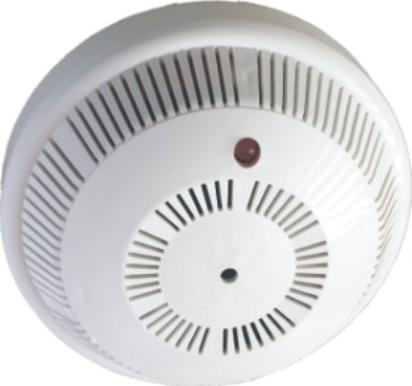
\includegraphics[scale=0.85]{avt_pozh_izv.jpg}  
    \caption{}
  \end{subfigure}
  \begin{subfigure}[b]{0.45\textwidth} 
    \centering
    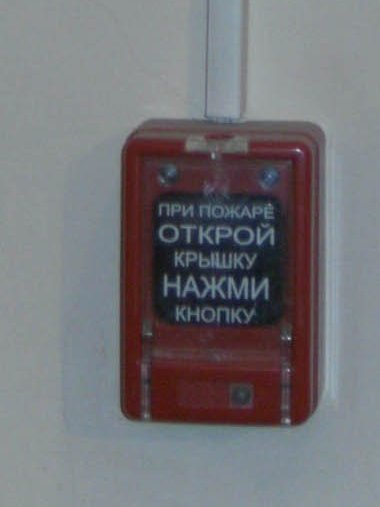
\includegraphics[scale=1.2]{ruch_pozh_izv.jpg}  
    \caption{}
  \end{subfigure}
  \caption{ а "--- автономный пожарный извещатель;
            б "--- ручной пожарный извещатель.}
  \label{fig:fire_alarms}
\end{figure}

На случай возникновения пожара в каждом рабочем кабинете находиться ручной порошковый огнетушитель \mbox{ОП-10}~(з)~МИГ~М (рисунок~\ref{fig:extinguishing_fire}), пригодный для тушения пожаров различного типа, в том числе для тушения электрических приборов~\cite[\ignore{раздел 5.5.7,} с.~221\,--\,323]{michnuk_2009}.
Каждый этаж здания офиса оборудован двумя пожарными кранами для тушения пожара.
Пожарные краны расположены в противоположных частях коридора, недалеко от эвакуационных выходов (рисунок~\ref{fig:extinguishing_fire}).
На случай воспламенения электрической проводки или другого электрического оборудования в каждом кабинете установлены электрические щитки, необходимые для отключения подачи электроэнергии в пределах кабинета.
Во всех помещениях офиса предприятия установлена оросительная система пожаротушения для ликвидации возгорания до приезда пожарной службы~\cite[\ignore{раздел~5.5.6,} с.~318\,--\,320]{michnuk_2009}.
При расследовании возможных причин возникновения пожара может быть задействована система видео"=наблюдения, установленная во всех помещениях предприятия.

\begin{figure}[ht]
\centering
  \begin{subfigure}[b]{0.45\textwidth} 
    \centering
    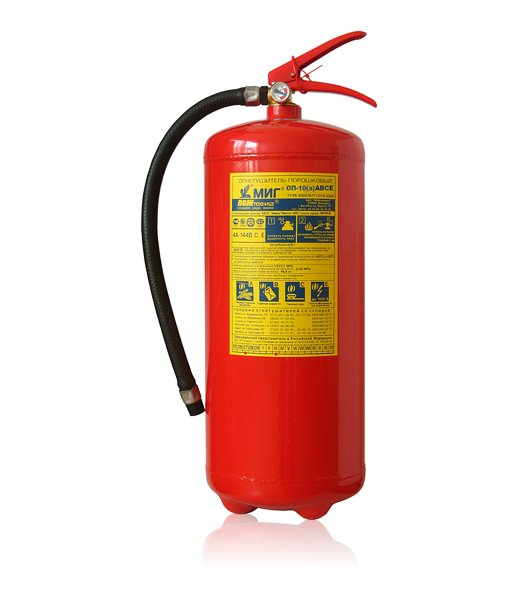
\includegraphics[scale=0.34]{ognetush.jpg}  
    \caption{}
  \end{subfigure}
  \begin{subfigure}[b]{0.45\textwidth} 
    \centering
    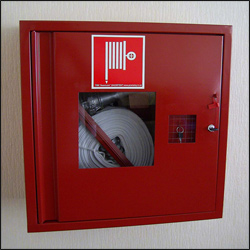
\includegraphics[scale=0.7]{pozh_kran.jpg}  
    \caption{}
  \end{subfigure}
  \caption{ а "--- порошковый огнетушитель \mbox{ОП-10}~(з)~МИГ~М;
            б "--- пожарный кран.}
  \label{fig:extinguishing_fire}
\end{figure}

Основной род деятельности на предприятии "--- разработка информационных систем "--- не предусматривает непосредственный контакт с горючими или легко"=воспламеняющимися веществами, что сильно снижает риски возникновения пожара на предприятии.
Наиболее вероятными причинами возникновения пожара, с учетом специфики предприятия, могут являться нарушение правил внутреннего распорядка "--- курение на рабочем месте, и неисправность электрического оборудования, которого в офисе компании достаточно~\cite[\ignore{раздел 5.5.1,} с.~312]{michnuk_2009}.
С целью снижения риска возникновения пожара по причине неисправности электрического оборудования в компании запрещено пользоваться неисправным оборудованием, а все исправное оборудование подключается в сеть через специальные сетевые фильтры и источники бесперебойного питания.
В целом правила распорядка на предприятии и высокая культура работы с электрическим оборудованием снижают риски возникновения пожара до минимума.

Большой проблемой в достижении максимальной пожарной безопасности предприятия является доступность подъезда пожарной техники к зданию офиса.
В будние дни прилегающие улицы, стоянки, пешеходные переходы заняты неправильно припаркованным личным транспортом.
Большую часть светлого времени суток движение по прилегающим улицам очень затруднено.
Данную проблему предприятие не в силах решить самостоятельно, проблема заключается в низкой культуре владельцев транспорта и игнорировании многочисленных нарушений правил дорожного движения  сотрудниками ГАИ.
% Заключительное предложение
Таким образом, изложенные выше предложения, не смотря на проблемы с подъездом пожарной техники, обеспечат пожарную безопасность на предприятии \companyname{}.


\newcommand{\byr}{Br}

\section{Технико-экономическое обоснование разработки ПС}

% Begin Calculations

\FPeval{\totalProgramSize}{16025}
\FPeval{\totalProgramSizeCorrected}{14490}

\FPeval{\normativeManDays}{306} %Tn

\FPeval{\additionalComplexity}{0.20} %Ksl
\FPeval{\complexityFactor}{clip(1 + \additionalComplexity)}

\FPeval{\stdModuleUsageFactor}{0.9} %Kt
\FPeval{\originalityFactor}{0.7} %Kn

\FPeval{\adjustedManDaysExact}{clip( \normativeManDays * \complexityFactor * \stdModuleUsageFactor * \originalityFactor )}
\FPround{\adjustedManDays}{\adjustedManDaysExact}{0}

\FPeval{\daysInYear}{366}
\FPeval{\redLettersDaysInYear}{6}
\FPeval{\weekendDaysInYear}{105}
\FPeval{\vocationDaysInYear}{24}
\FPeval{\workingDaysInYear}{ clip( \daysInYear - \redLettersDaysInYear - \weekendDaysInYear - \vocationDaysInYear ) }

\FPeval{\developmentTimeMonths}{6}
\FPeval{\developmentTimeYearsExact}{clip(\developmentTimeMonths / 12)}
\FPround{\developmentTimeYears}{\developmentTimeYearsExact}{2}
\FPeval{\requiredNumberOfProgrammersExact}{ clip( \adjustedManDays / (\developmentTimeYears * \workingDaysInYear) + 0.5 ) }

% тут должно получаться 2 ))
\FPtrunc{\requiredNumberOfProgrammers}{\requiredNumberOfProgrammersExact}{0}

\FPeval{\tariffRateFirst}{298000} %Tm1
\FPeval{\tariffFactorFst}{3.04}
\FPeval{\tariffFactorSnd}{3.48}


\FPeval{\employmentFstExact}{clip( \adjustedManDays / \requiredNumberOfProgrammers )}
\FPtrunc{\employmentFst}{\employmentFstExact}{0}

\FPeval{\employmentSnd}{clip(\adjustedManDays - \employmentFst)}


\FPeval{\workingHoursInMonth}{160} %Fr
\FPeval{\salaryPerHourFstExact}{clip( \tariffRateFirst * \tariffFactorFst / \workingHoursInMonth )}
\FPeval{\salaryPerHourSndExact}{clip( \tariffRateFirst * \tariffFactorSnd / \workingHoursInMonth )}
\FPround{\salaryPerHourFst}{\salaryPerHourFstExact}{0}
\FPround{\salaryPerHourSnd}{\salaryPerHourSndExact}{0}

\FPeval{\bonusRate}{1.5}
\FPeval{\workingHoursInDay}{8}
\FPeval{\totalSalaryExact}{clip( \workingHoursInDay * \bonusRate * ( \salaryPerHourFst * \employmentFst + \salaryPerHourSnd * \employmentSnd ) )}
\FPround{\totalSalary}{\totalSalaryExact}{0}

\FPeval{\additionalSalaryNormative}{20}

\FPeval{\additionalSalaryExact}{clip( \totalSalary * \additionalSalaryNormative / 100 )}
\FPround{\additionalSalary}{\additionalSalaryExact}{0}

\FPeval{\socialNeedsNormative}{0.5}
\FPeval{\socialProtectionNormative}{34.5}
\FPeval{\socialProtectionFund}{ clip(\socialNeedsNormative + \socialProtectionNormative) }

\FPeval{\socialProtectionCostExact}{clip( (\totalSalary + \additionalSalary) * \socialProtectionFund / 100 )}
\FPround{\socialProtectionCost}{\socialProtectionCostExact}{0}

\FPeval{\stuffNormative}{3}
\FPeval{\stuffCostExact}{clip( \totalSalary * \stuffNormative / 100 )}
\FPround{\stuffCost}{\stuffCostExact}{0}

\FPeval{\timeToDebugCodeNormative}{15}
%\FPeval{\reducingTimeToDebugFactor}{0.3} %?
\FPeval{\adjustedTimeToDebugCodeNormative}{\timeToDebugCodeNormative}

\FPeval{\oneHourMachineTimeCost}{2400}

\FPeval{\machineTimeCostExact}{ clip( \oneHourMachineTimeCost * \totalProgramSizeCorrected / 100 * \adjustedTimeToDebugCodeNormative ) }
\FPround{\machineTimeCost}{\machineTimeCostExact}{0}

\FPeval{\businessTripNormative}{15}
\FPeval{\businessTripCostExact}{ clip( \totalSalary * \businessTripNormative / 100 ) }
\FPround{\businessTripCost}{\businessTripCostExact}{0}

\FPeval{\otherCostNormative}{20}
\FPeval{\otherCostExact}{clip( \totalSalary * \otherCostNormative / 100 )}
\FPround{\otherCost}{\otherCostExact}{0}

\FPeval{\overheadCostNormative}{100}
\FPeval{\overallCostExact}{clip( \totalSalary * \overheadCostNormative / 100 )}
\FPround{\overheadCost}{\overallCostExact}{0}

\FPeval{\overallCost}{clip( \totalSalary + \additionalSalary + \socialProtectionCost + \stuffCost + \machineTimeCost + \businessTripCost + \otherCost + \overheadCost ) }

\FPeval{\supportNormative}{30}
\FPeval{\softwareSupportCostExact}{clip( \overallCost * \supportNormative / 100 )}
\FPround{\softwareSupportCost}{\softwareSupportCostExact}{0}


\FPeval{\baseCost}{ clip( \overallCost + \softwareSupportCost ) }

\FPeval{\profitability}{35}
\FPeval{\incomeExact}{clip( \baseCost / 100 * \profitability )}
\FPround{\income}{\incomeExact}{0}

\FPeval{\estimatedPrice}{clip( \income + \baseCost )}

\FPeval{\localRepubTaxNormative}{3.9}
\FPeval{\localRepubTaxExact}{clip( \estimatedPrice * \localRepubTaxNormative / (100 - \localRepubTaxNormative) )}
\FPround{\localRepubTax}{\localRepubTaxExact}{0}
%\FPeval{\localRepubTax}{0}

\FPeval{\ndsNormative}{20}
\FPeval{\ndsExact}{clip( (\estimatedPrice + \localRepubTax) / 100 * \ndsNormative )}
\FPround{\nds}{\ndsExact}{0}


\FPeval{\sellingPrice}{clip( \estimatedPrice + \localRepubTax + \nds )}

\FPeval{\taxForIncome}{18}
\FPeval{\incomeWithTaxesExact}{clip(\income * (1 - \taxForIncome / 100))}
\FPround{\incomeWithTaxes}{\incomeWithTaxesExact}{0}

% End Calculations

Целью дипломного проекта является создание программного средства для обфускации исходных кодов проектных описаний, написанныъ на языке VHDL.
Данное программное средство позволяет усложнить чтение злоумышленником как исходных кодов программы(лексическая обфускация), так и результата их синтеза(функциональная обфускация). Данное программное средство обладает рядом достоинств: позволяет проверять правильность исходного кода на предварительном этапе, имеет возможность интеграции с другими инструментами разработки, позволяет проводить только лексическую или только функциональную обфускацию, или обе сразу.

Расчеты выполнены на основе методического пособия ~\cite{palicyn_2006}.

\subsection{Расчёт сметы затрат и цены программного продукта}

Целесообразность создания коммерческого ПО требует проведения предварительной экономической оценки и расчета экономического эффекта.
Экономический эффект у разработчика ПО зависит от объёма инвестиций в разработку проекта, цены на готовый программный продукт и количества проданных копий, и проявляется в виде роста чистой прибыли.

Исходные данные для разрабатываемого проекта указаны в таблице~\ref{table:econ:initial_data}.

\begin{table}[!ht]
\caption{Исходные данные}
\label{table:econ:initial_data}
  \centering
  \begin{tabular}{| >{\raggedright}m{0.62\textwidth}
                  | >{\centering}m{0.17\textwidth}
                  | >{\centering\arraybackslash}m{0.13\textwidth}|}
    \hline
    {\begin{center}
      Наименование
    \end{center} } & Условное обозначение & Значение \\
    \hline
    Категория сложности & & 2 \\

    \hline
    Коэффициент сложности, ед. & $ \text{К}_\text{с} $ & \num{\complexityFactor} \\

    \hline
    Степень использования при разработке стандартных модулей, ед. & $ \text{К}_\text{т} $ & \num{\stdModuleUsageFactor} \\

    \hline
    Коэффициент новизны, ед. & $ \text{К}_\text{н} $ & \num{\originalityFactor} \\

    \hline
    Годовой эффективный фонд времени, дн. & $ \text{Ф}_\text{эф} $ & \num{\workingDaysInYear} \\

    \hline
    Продолжительность рабочего дня, ч. & $ \text{Т}_\text{ч} $ & \num{\workingHoursInDay} \\

    \hline
    Месячная тарифная ставка первого разряда, \byr{} & $ \text{Т}_{\text{м}_{1}}$ & \num{\tariffRateFirst} \\

    \hline
    Коэффициент премирования, ед. & $ \text{К} $ & \num{\bonusRate} \\

    \hline
    Норматив дополнительной заработной платы, ед. & $ \text{Н}_\text{д} $ & \num{\additionalSalaryNormative} \\

    \hline
    Норматив отчислений в ФСЗН и обязательное страхование, $\%$ & $ \text{Н}_\text{сз} $ & \num{\socialProtectionFund} \\

    \hline
    Норматив командировочных расходов, $\%$ & $ \text{Н}_\text{к} $ & \num{\businessTripNormative} \\

    \hline
    Норматив прочих затрат, $\%$ & $ \text{Н}_\text{пз} $ & \num{\otherCostNormative} \\

    \hline
    Норматив накладных расходов, $\%$ & $ \text{Н}_\text{рн} $ & \num{\overheadCostNormative} \\

    \hline
    Прогнозируемый уровень рентабельности, $\%$ & $ \text{У}_\text{рп} $ & \num{\profitability} \\

    \hline
    Норматив НДС, $\%$ & $ \text{Н}_\text{дс} $ & \num{\ndsNormative} \\

    \hline
    Норматив налога на прибыль, $\%$ & $ \text{Н}_\text{п} $ & \num{\taxForIncome} \\

    \hline
    Норматив расхода материалов, $\%$ & $ \text{Н}_\text{мз} $ & \num{\stuffNormative} \\

    \hline
    Норматив расхода машинного времени, ч. & $ \text{Н}_\text{мв} $ & \num{\adjustedTimeToDebugCodeNormative} \\

    \hline
    Цена одного часа машинного времени, \byr{} & $ \text{Н}_\text{мв} $ & \num{\oneHourMachineTimeCost} \\

    \hline
    Норматив расходов на сопровождение и адаптацию ПО, $\%$ & $ \text{Н}_\text{рса} $ & \num{\supportNormative} \\
    \hline
  \end{tabular}
\end{table}

На основании сметы затрат и анализа рынка ПО определяется плановая отпускаемая цена.
Для составления сметы затрат на создание ПО необходима предварительная оценка трудоемкости ПО и его объёма.
Расчет объёма программного продукта (количества строк исходного кода) предполагает определение типа программного обеспечения, всестороннее техническое обоснование функций ПО и определение объёма каждой функций.
Согласно классификации типов программного обеспечения~\cite[с.~59,~приложение 1]{palicyn_2006}, разрабатываемое ПО с наименьшей ошибкой можно классифицировать как ПО методo"=ориентированных расчетов.

В данном разделе рассмотрим экономическую эффективность программного средства. Программный комплекс относится ко 2-ой группе сложности. Категория новизны продукта - «В».
Для оценки экономической эффективности разработанного программного средства проводится расчет цены и прибыли от продажи одной системы(программы).

Общий объём программного продукта определяется исходя из количества и объёма функций, реализованных в программе:
\begin{equation}
  \label{eq:econ:total_program_size}
  V_{o} = \sum_{i = 1}^{n} V_{i} \text{\,,}
\end{equation}
\begin{explanation}
где & $ V_{i} $ & объём отдельной функции ПО, LoC; \\
    & $ n $ & общее число функций.
\end{explanation}

На стадии технико-экономического обоснования проекта рассчитать точный объём функций невозможно.
Вместо вычисления точного объёма функций применяются приблизительные оценки на основе данных по аналогичным проектам или по нормативам~\cite[с.~61,~приложение 2]{palicyn_2006}, которые приняты в организации.

\begin{table}[ht]
\caption{Перечень и объём функций программного модуля}
\label{table:econ:function_sizes}
\centering
  \begin{tabular}{| >{\centering}m{0.12\textwidth}
                  | >{\raggedright}m{0.40\textwidth}
                  | >{\centering}m{0.18\textwidth}
                  | >{\centering\arraybackslash}m{0.18\textwidth}|}

  \hline
         \multirow{2}{0.12\textwidth}[-0.5em]{\centering \No{} функции}
       & \multirow{2}{0.40\textwidth}[-0.55em]{\centering Наименование (содержание)}
       & \multicolumn{2}{c|}{\centering Объём функции, LoC} \tabularnewline

  \cline{3-4} &
       & { по каталогу ($ V_{i} $) }
       & { уточненный ($ V_{i}^{\text{у}} $) } \tabularnewline

  \hline
  101 & Организация ввода информации & \num{85} & \num{60} \tabularnewline

  \hline
  102 & Контроль, предварительная обработка и ввод информации & \num{300} & \num{250} \tabularnewline

  \hline
  103 & Анализ входного языка(синтаксический и семантический) & \num{700} & \num{690} \tabularnewline

  \hline
  107 & Синтаксический и семантический анализ входного языка и генерация кодов команд & \num{9000} & \num{7800} \tabularnewline

  \hline
  108 & Процессор языка & \num{3500} & \num{3200} \tabularnewline

  \hline
  109 & Организация ввода/вывода информации с интерактивном режиме & \num{200} & \num{150} \tabularnewline

  \hline
  305 & Обработка файлов & \num{300} & \num{2500} \tabularnewline

  \hline
  309 & Формирование файла & \num{1000} & \num{900} \tabularnewline

  \hline
  506 & Обработка ошибочных и сбойных ситуаций & \num{400} & \num{300} \tabularnewline

  \hline
  507 & Обеспечение интерфейса между компонентами & \num{900} & \num{890} \tabularnewline

  \hline

  % Уточенная оценка вычислялась с помощью R: (+ручной фикс)
  % set.seed(35)
  % locs <- c(100, 520, 2700, 520, 750, 1100, 430, 730, 460, 8370)
  % locs.which.corrected <- rbinom(length(locs), 1, 0.4)
  % locs.corrections <- rnorm(length(locs), mean = -0.25, sd=0.3)
  % locs.correction.factor <- 1 + locs.which.corrected * locs.corrections
  % locs.corrected <- signif(locs * locs.correction.factor, digits = 2)
  % locs.corrected
  % sum(locs)
  % sum(locs.corrected)

  Итог & & {\num{\totalProgramSize}} & {\num{\totalProgramSizeCorrected}} \tabularnewline

  \hline

  \end{tabular}
\end{table}

Перечень и объём функций программного модуля перечислен в таблице~\ref{table:econ:function_sizes}.
По приведенным данным уточненный объём некоторых функций изменился, и общий уточненный объём ПО $ V_{\text{у}} = \SI{\totalProgramSizeCorrected}{\text{LoC}} $.

\subsection{Расчёт нормативной трудоемкости}

На основании общего объема ПО определяется нормативная трудоемкость ($ \text{Т}_\text{н}$) с учетом сложности ПО. Для ПО 2-ой группы сложности, к которой относится разрабатываемый программный продукт, нормативная трудоемкость составит~$ \text{Т}_\text{н} = \SI{\normativeManDays}{\text{чел.} / \text{дн.}}  $

Нормативная трудоемкость служит основой для оценки общей трудоемкости~$ \text{Т}_\text{о} $.
Используем формулу (\ref{eq:econ:effort_common}) для оценки общей трудоемкости для небольших проектов:
\begin{equation}
  \label{eq:econ:effort_common}
  \text{Т}_\text{о} = \text{Т}_\text{н} \cdot
                      \text{К}_\text{с} \cdot
                      \text{К}_\text{т} \cdot
                      \text{К}_\text{н} \text{\,,}
\end{equation}
\begin{explanation}
где & $ \text{К}_\text{с} $ & коэффициент, учитывающий сложность ПО; \\
    & $ \text{К}_\text{т} $ & поправочный коэффициент, учитывающий степень использования при разработке стандартных модулей; \\
    & $ \text{К}_\text{н} $ & коэффициент, учитывающий степень новизны ПО.
\end{explanation}

Дополнительные затраты труда на разработку ПО учитываются через коэффициент сложности, который вычисляется по формуле
\begin{equation}
\label{eq:econ:complexity_coeff}
  \text{К}_{\text{с}} = 1 + \sum_{i = 1}^n \text{К}_{i} \text{\,,}
\end{equation}
\begin{explanation}
где & $ \text{К}_{i} $ & коэффициент, соответствующий степени повышения сложности ПО за счет конкретной характеристики; \\
    & $ n $ & количество учитываемых характеристик.
\end{explanation}

Наличие двух характеристик сложности позволяет~\cite[c.~66, приложение~4, таблица~П.4.2]{palicyn_2006} вычислить коэффициент сложности
\begin{equation}
\label{eq:econ:complexity_coeff_calc}
  \text{К}_{\text{с}} = \num{1} + \num{\additionalComplexity} = \num{\complexityFactor} \text{\,.}
\end{equation}

Разрабатываемое ПО использует стандартные компоненты. Согласно справочным данным~\cite[c.~68,~приложение~4, таблица~П.4.5]{palicyn_2006} коэффициент использования стандартных модулей для разрабатываемого приложения $ \text{К}_\text{т} = \num{\stdModuleUsageFactor} $.
Разрабатываемое ПО не является новым, существуют аналогичные более зрелые разработки у различных компаний и университетов по всему миру.
Влияние степени новизны на трудоемкость создания ПО определяется коэффициентом новизны~---~$ \text{К}_\text{н} $.
Согласно справочным данным~\cite[c.~67, приложение~4, таблица~П.4.4]{palicyn_2006} для разрабатываемого ПО $ \text{К}_\text{н} = \num{\originalityFactor} $.
Подставив приведенные выше коэффициенты для разрабатываемого ПО в формулу~(\ref{eq:econ:effort_common}) получим общую трудоемкость разработки
\begin{equation}
  \label{eq:econ:effort_common_calc}
  \text{Т}_\text{о} = \num{\normativeManDays} \times \num{\complexityFactor} \times \num{\stdModuleUsageFactor} \times \num{\originalityFactor} \approx \SI{\adjustedManDays}{\text{чел.}/\text{дн.}}
\end{equation}

На основе общей трудоемкости и требуемых сроков реализации проекта вычисляется плановое количество исполнителей.
Численность исполнителей проекта рассчитывается по формуле:
\begin{equation}
  \label{eq:econ:num_of_programmers}
  \text{Ч}_\text{р} = \frac{\text{Т}_\text{о}}{\text{Т}_\text{р} \cdot \text{Ф}_\text{эф}} \text{\,,}
\end{equation}
\begin{explanation}
где & $ \text{Т}_\text{о} $ & общая трудоемкость разработки проекта, $ \text{чел.}/\text{дн.} $; \\
    & $ \text{Ф}_\text{эф} $ & эффективный фонд времени работы одного работника в течение года, дн.; \\
    & $ \text{Т}_\text{р} $ & срок разработки проекта, лет.
\end{explanation}

Эффективный фонд времени работы одного разработчика вычисляется по формуле
\begin{equation}
  \label{eq:econ:effective_time_per_programmer}
  \text{Ф}_\text{эф} =
    \text{Д}_\text{г} -
    \text{Д}_\text{п} -
    \text{Д}_\text{в} -
    \text{Д}_\text{о} \text{\,,}
\end{equation}
\begin{explanation}
где & $ \text{Д}_\text{г} $ & количество дней в году, дн.; \\
    & $ \text{Д}_\text{п} $ & количество праздничных дней в году, не совпадающих с выходными днями, дн.; \\
    & $ \text{Д}_\text{в} $ & количество выходных дней в году, дн.; \\
    & $ \text{Д}_\text{п} $ & количество дней отпуска, дн.
\end{explanation}

Согласно данным, приведенным в производственном календаре для пятидневной рабочей недели в 2016 году для Беларуси~\cite{belcalendar_2016}, фонд рабочего времени составит
\begin{equation}
  \text{Ф}_\text{эф} = \num{\daysInYear} - \num{\redLettersDaysInYear} - \num{\weekendDaysInYear} - \num{\vocationDaysInYear} = \SI{\workingDaysInYear}{\text{дн.}}
\end{equation}

Учитывая срок разработки проекта $ \text{Т}_\text{р} = \SI{\developmentTimeMonths}{\text{мес.}} = \SI{\developmentTimeYears}{\text{года}} $, общую трудоемкость и фонд эффективного времени одного работника, вычисленные ранее, можем рассчитать численность исполнителей проекта
\begin{equation}
  \label{eq:econ:num_of_programmers_calc}
  \text{Ч}_\text{р} =
    \frac{\num{\adjustedManDays}}
         {\num{\developmentTimeYears} \times \num{\workingDaysInYear}}
    \approx \SI{\requiredNumberOfProgrammers}{\text{рабочих}}.
\end{equation}

Вычисленные оценки показывают, что для выполнения запланированного проекта в указанные сроки необходимо два рабочих.

\subsection{Расчёт основной заработной платы исполнителей}

Информация о работниках перечислена в таблице~\ref{table:econ:programmers}.
\begin{table}[ht]
  \caption{Работники, занятые в проекте}
  \label{table:econ:programmers}
  \begin{tabular}{| >{\centering}m{0.4\textwidth}
                  | >{\centering}m{0.15\textwidth}
                  | >{\centering}m{0.18\textwidth}
                  | >{\centering\arraybackslash}m{0.15\textwidth}|}
   \hline
   Исполнители & Разряд & Тарифный коэффициент & \mbox{Чел./дн.} занятости \\
   \hline
   Программист \Rmnum{1}-категории & $ \num{13} $ & $ \num{\tariffFactorFst} $ & $ \num{\employmentFst} $ \\
   \hline
   Ведущий программист & $ \num{15} $ & $ \num{\tariffFactorSnd} $ & $ \num{\employmentSnd} $ \\
   \hline
  \end{tabular}
\end{table}

Месячная тарифная ставка одного работника вычисляется по формуле
\begin{equation}
  \label{eq:econ:month_salary}
  \text{Т}_\text{ч} =
    \frac {\text{Т}_{\text{м}_{1}} \cdot \text{Т}_{\text{к}} }
          {\text{Ф}_{\text{р}} }  \text{\,,}
\end{equation}
\begin{explanation}
где & $ \text{Т}_{\text{м}_{1}} $ & месячная тарифная ставка 1-го разряда, \byr; \\
    & $ \text{Т}_{\text{к}} $ & тарифный коэффициент, соответствующий установленному тарифному разряду; \\
    & $ \text{Ф}_{\text{р}} $ & среднемесячная норма рабочего времени, час.
\end{explanation}




Подставив данные из таблицы~\ref{table:econ:programmers} в формулу~(\ref{eq:econ:month_salary}), приняв значение тарифной ставки 1-го разряда $ \text{Т}_{\text{м}_{1}} = \SI{\tariffRateFirst}{\text{\byr}} $ и среднемесячную норму рабочего времени $ \text{Ф}_{\text{р}} = \SI{\workingHoursInMonth}{\text{часов}} $ получаем
\begin{equation}
  \label{eq:econ:month_salary_calc1}
  \text{Т}_{\text{ч}}^{\text{прогр. \Rmnum{1}-разр.}} = \frac{ \num{\tariffRateFirst} \times \num{\tariffFactorFst} } { \num{\workingHoursInMonth} } = \SI{\salaryPerHourFst}{\text{\byr}/\text{час;}}
\end{equation}
\begin{equation}
  \label{eq:econ:month_salary_calc2}
  \text{Т}_{\text{ч}}^{\text{вед. прогр.}} = \frac{ \num{\tariffRateFirst} \times \num{\tariffFactorSnd} } { \num{\workingHoursInMonth} } = \SI{\salaryPerHourSnd}{\text{\byr}/\text{час.}}
\end{equation}

Основная заработная плата исполнителей на конкретное ПО рассчитывается по формуле
\begin{equation}
  \label{eq:econ:total_salary}
  \text{З}_{\text{о}} = \sum^{n}_{i = 1}
                        \text{Т}_{\text{ч}}^{i} \cdot
                        \text{Т}_{\text{ч}} \cdot
                        \text{Ф}_{\text{п}} \cdot
                        \text{К}
                          \text{\,,}
\end{equation}
\begin{explanation}
где & $ \text{Т}_{\text{ч}}^{i} $ & часовая тарифная ставка \mbox{$ i $-го} исполнителя, \byr$/$час; \\
    & $ \text{Т}_{\text{ч}} $ & количество часов работы в день, час; \\
    & $ \text{Ф}_{\text{п}} $ & плановый фонд рабочего времени \mbox{$ i $-го} исполнителя, дн.; \\
    & $ \text{К} $ & коэффициент премирования.
\end{explanation}

Подставив ранее вычисленные значения и данные из таблицы~\ref{table:econ:programmers} в формулу~(\ref{eq:econ:total_salary}) и приняв коэффициент премирования $ \text{К} = \num{\bonusRate} $ получим
\begin{equation}
  \label{eq:econ:total_salary_calc}
  \text{З}_{\text{о}} = (\salaryPerHourFst \times \num{\employmentFst} + \salaryPerHourSnd \times \num{\employmentSnd}) \times \num{\workingHoursInDay} \times \num{\bonusRate} = \SI{\totalSalary}{\text{\byr}} \text{\,.}
\end{equation}

Дополнительная заработная плата включает выплаты предусмотренные законодательством от труде и определяется по нормативу в процентах от основной заработной платы
\begin{equation}
  \label{eq:econ:additional_salary}
  \text{З}_{\text{д}} =
    \frac {\text{З}_{\text{о}} \cdot \text{Н}_{\text{д}}}
          {100\%} \text{\,,}
\end{equation}
\begin{explanation}
  где & $ \text{Н}_{\text{д}} $ & норматив дополнительной заработной платы, $ \% $.
\end{explanation}

Приняв норматив дополнительной заработной платы $ \text{Н}_{\text{д}} = \num{\additionalSalaryNormative\%} $ и подставив известные данные в формулу~(\ref{eq:econ:additional_salary}) получим
\begin{equation}
  \label{eq:econ:additional_salary_calc}
  \text{З}_{\text{д}} =
    \frac{\num{\totalSalary} \times 20\%}
         {100\%} \approx \SI{\additionalSalary}{\text{\byr}} \text{\,.}
\end{equation}

Расчеты общей суммы расходов и прогнозируемой цены ПО, а также его себестоимости сведены в таблицу~\ref{table:econ:calculation_cost_and_price}.

\begin{longtable}{| >{\raggedright}m{0.27\textwidth}
                  | >{\centering}m{0.16\textwidth}
                  | >{\centering}m{0.35\textwidth}
                  | >{\centering\arraybackslash}m{0.15\textwidth}|}
  \caption{Расчет себестоимости и отпускной цены ПО}
  \label{table:econ:calculation_cost_and_price}

  \hline
    {\begin{center}
       Наименование статей
    \end{center} } & \mbox{Норматив,} \% & Методика расчета & \mbox{Значение,} руб. \\
   \hline
   Отчисления в фонд социальной защиты и обязательного страхования
   & $ \text{Н}_{\text{сз}} = \num{\socialProtectionFund} $
   & $ \text{З}_{\text{сз}} = (\text{З}_{\text{о}} + \text{З}_{\text{д}}) \cdot \text{Н}_{\text{сз}} / {\num{100}} $
   & \num{\socialProtectionCost}\\
   \hline
   Материалы и комплектующие
   & $ \text{Н}_{\text{мз}} = \num{\stuffNormative} $
   & $\text{М} = { \text{З}_{\text{о}} \cdot \text{Н}_{\text{мз}} } / { \num{100} } $
   & \num{\stuffCost} \\
   \hline
   Машинное время
   &
   & $ \text{Р}_{\text{м}} = \text{Ц}_{\text{м}} \cdot \text{V}_{\text{о}} / \num{100} \cdot \text{Н}_{\text{мв}} $
   $ \text{Н}_{\text{мв}} = \num{\timeToDebugCodeNormative}{\text{ машино-часов}}$
   $ \text{Ц}_{\text{м}} = \SI{\oneHourMachineTimeCost}{\text{\byr}} $
   & \num{\machineTimeCost} \\
   \hline
   Расходы на научные командировки
   & $ \text{Н}_{\text{к}} = \num{\businessTripNormative} $
   & $  \text{Р}_{\text{к}} = { \text{З}_{\text{о}} \cdot \text{Н}_{\text{к}} } / \num{100} $
   & \num{\businessTripCost} \\
   \hline
   Прочие прямые расходы
   & $ \text{Н}_{\text{пз}} = \num{\otherCostNormative} $
   & $  \text{П}_{\text{з}} = { \text{З}_{\text{о}} \cdot \text{Н}_{\text{пз}} } / \num{100} $
   & \num{\otherCost} \\
   \hline
   Накладные расходы
   & $ \text{Н}_{\text{рн}} = \num{\overheadCostNormative} $
   & $  \text{Р}_{\text{н}} = { \text{З}_{\text{о}} \cdot \text{Н}_{\text{рн}} } / \num{100} $
   & \num{\overheadCost}\\
   \hline
   Общая сумма расходов по смете
   &
   & $  \text{С}_{\text{р}} = \text{З}_{\text{о}} + \text{З}_{\text{д}} + \text{З}_{\text{сз}} + \text{М} + \text{Р}_{\text{м}} + \text{Р}_{\text{к}} + \text{П}_{\text{з}} + \text{Р}_{\text{н}} $
   & \num{\overallCost}\\
   \hline
   Сопровождение и адаптация ПО
   & $ \text{Н}_{\text{рса}} = \num{\supportNormative} $
   & $  \text{Р}_{\text{са}} = {\text{С}_{\text{р}} \cdot \text{Н}_{\text{рса}} } / { \num{100} } $
   & \num{\softwareSupportCost} \\
   \hline
   Полная себестоимость ПО
   &
   & $ \text{С}_{\text{п}} = \text{С}_{\text{р}} + \text{Р}_{\text{са}} $
   & \num{\baseCost} \\
   \hline
   Прогнозируемая прибыль
   & $ \text{У}_{\text{рп}} = \num{\profitability} $
   & $  \text{П}_{\text{с}} = { \text{С}_{\text{п}} \cdot \text{У}_{\text{рп}} } / \num{100} $
   & \num{\income} \\

   %-----------------------------------------
  \caption*{Продолжение таблицы~\ref{table:econ:calculation_cost_and_price}}
  \hline
    {\begin{center}
       Наименование статей
    \end{center} } & \mbox{Норматив,} \% & Методика расчета & \mbox{Значение,} руб. \\
   \hline
   Прогнозируемая цена без налогов
   &
   & $ \text{Ц}_{\text{п}} = \text{С}_{\text{п}} + \text{П}_{\text{с}}$
   & \num{\estimatedPrice} \\
   \hline
   Отчисления и налоги в местный и республиканский бюджеты
   & $ \text{Н}_{\text{мр}} = \num{\localRepubTaxNormative} $
   & $ \text{О}_{\text{мр}} = { \text{Ц}_{\text{п}} \cdot \text{Н}_{\text{мр}} } / { \num{100} - \text{Н}_{\text{мр}} } $
   & \num{\localRepubTax} \\
   \hline
   Налог на добавленную стоимость
   & $ \text{Н}_{\text{дс}} = \num{\ndsNormative} $
   & $ \text{НДС}_{\text{}} = { (\text{Ц}_{\text{п}} + \text{О}_{\text{мр}}) \cdot \text{Н}_{\text{дс}} } / \num{100} $
   & \num{\nds} \\
   \hline
   Прогнозируемая отпускная цена
   &
   & $ \text{Ц}_{\text{о}} = \text{Ц}_{\text{п}} + \text{О}_{\text{мр}} + \text{НДС} $
   & \num{\sellingPrice} \\
   \hline
\end{longtable}

\subsection{Расчёт экономической эффективности у разработчика}

Важная задача при выборе проекта для финансирования это расчет экономической эффективности проектов и выбор наиболее выгодного проекта.
Разрабатываемое ПО является заказным, т.е. разрабатывается для одного заказчика на заказ. На основании анализа рыночных условий и договоренности с заказчиком об отпускной цене прогнозируемая рентабельность проекта составит $ \text{У}_{\text{рп}} = \num{\profitability\%} $.

Чистую прибыль от реализации проекта можно рассчитать по формуле
\begin{equation}
  \label{eq:econ:income_with_taxes}
  \text{П}_\text{ч} =
    \text{П}_\text{c} \cdot
    \left(1 - \frac{ \text{Н}_\text{п} }{ \num{100\%} } \right) \text{\,,}
\end{equation}
\begin{explanation}
  где & $ \text{Н}_{\text{п}} $ & величина налога на прибыль,~$\%$.
\end{explanation}

Приняв значение налога на прибыль $ \text{Н}_{\text{н}} = \num{\taxForIncome\%} $ и подставив известные данные в формулу~(\ref{eq:econ:income_with_taxes}) получаем чистую прибыль
\begin{equation}
  \label{eq:econ:income_with_taxes_calc}
  \text{П}_\text{ч} =
    \num{\income} \times \left( 1 - \frac{\num{\taxForIncome\%}}{100\%} \right) = \SI{\incomeWithTaxes}{\text{\byr}} \text{\,.}
\end{equation}

Программное обеспечение разрабатывалось для одного заказчика в связи с этим экономическим эффектом разработчика будет являться чистая прибыль от реализации~$ \text{П}_\text{ч} $.
Рассчитанные данные приведены в таблице~\ref{table:econ:calculated_data}.

\begin{table}[!ht]
\caption{Рассчитанные данные}
\label{table:econ:calculated_data}
  \centering
  \begin{tabular}{| >{\raggedright}m{0.60\textwidth}
                  | >{\centering}m{0.17\textwidth}
                  | >{\centering\arraybackslash}m{0.15\textwidth}|}
    \hline
    {\begin{center}
      Наименование
    \end{center} } & Условное обозначение & Значение \\
    \hline
    Нормативная трудоемкость, чел.$/$дн. & $ \text{Т}_\text{н} $ & \num{\normativeManDays} \\

    \hline
    Общая трудоемкость разработки, чел.$/$дн. & $ \text{Т}_\text{о} $ & \num{\adjustedManDays} \\

    \hline
    Численность исполнителей, чел. & $ \text{Ч}_\text{р} $ & \num{\requiredNumberOfProgrammers} \\

    \hline
    Часовая тарифная ставка программиста \Rmnum{1}-разряда, \byr{}$/$ч. & $ \text{Т}_{\text{ч}}^{\text{прогр. \Rmnum{1}-разр.}} $ & \num{\salaryPerHourFst} \\

    \hline
    Часовая тарифная ставка ведущего программиста, \byr{}$/$ч. & $ \text{Т}_{\text{ч}}^{\text{вед. прогр.}} $ & \num{\salaryPerHourSnd} \\

    \hline
    Основная заработная плата, \byr{} & $ \text{З}_\text{о} $ & \num{\totalSalary} \\

    \hline
    Дополнительная заработная плата, \byr{} & $ \text{З}_\text{д}$ & \num{\additionalSalary} \\

    \hline
    Отчисления в фонд социальной защиты, \byr{} & $ \text{З}_\text{сз} $ & \num{\socialProtectionCost} \\

    \hline
    Затраты на материалы, \byr{} & $ \text{М} $ & \num{\stuffCost} \\

    \hline
    Расходы на машинное время, \byr{} & $ \text{Р}_\text{м} $ & \num{\machineTimeCost} \\

    \hline
    Расходы на командировки, \byr{} & $ \text{Р}_\text{к} $ & \num{\businessTripCost} \\

    \hline
    Прочие затраты, \byr{} & $ \text{П}_\text{з} $ & \num{\otherCost} \\

    \hline
    Накладные расходы, \byr{} & $ \text{Р}_\text{н} $ & \num{\overheadCost} \\

    \hline
    Общая сумма расходов по смете, \byr{} & $ \text{С}_\text{р} $ & \num{\overallCost} \\

    \hline
    Расходы на сопровождение и адаптацию, \byr{} & $ \text{Р}_\text{са} $ & \num{\softwareSupportCost} \\

    \hline
    Полная себестоимость, \byr{} & $ \text{С}_\text{п} $ & \num{\baseCost} \\

    \hline
    Прогнозируемая прибыль, \byr{} & $ \text{П}_\text{с} $ & \num{\income} \\

    \hline
    НДС, \byr{} & $ \text{НДС} $ & \num{\nds} \\

    \hline
    Прогнозируемая отпускная цена ПО, \byr{} & $ \text{Ц}_\text{о} $ & \num{\sellingPrice} \\

    \hline
    Чистая прибыль, \byr{} & $ \text{П}_\text{ч} $ & \num{\incomeWithTaxes} \\

    \hline
  \end{tabular}
\end{table}

\subsection{Выводы по технико-экономическому обоснованию}

Программное средство лексической и функциональной обфускации проектных описаний цифровых устройств является выгодным программным продуктом.
Чистая прибыль от реализации ПС ($ \text{П}_\text{ч} $ \num{\incomeWithTaxes} рублей) остается организации-разработчику и представляет собой экономический эффект от создания нового программного средства.
Прогнозируемая отпускная цена ($\text{Ц}_\text{о}$) составляет \num{\sellingPrice} рублей. Таким образом, данная разработка является экономически целесообразной.
В итоге было произведено технико-экономическое обоснование разрабатываемого проекта, составлена смета затрат и рассчитана прогнозируемая прибыль, а также показана экономическая целесообразность разработки.

\hfill
\clearpage

\sectioncentered*{Заключение}
\addcontentsline{toc}{section}{Заключение}

В данном дипломном проекте был рассмотрен вопрос лексического и синтаксического анализа языка VHDL, также различные методики запутывания, как исходного кода, так и результата синтеза этого кода. В рамках дипломного проекта была разработана библиотека кода для анализа и обфускации исходных кодов на языке VHDL.
В разработанном проекте был использован генератор парсеров YACC для создания анализатора языка, а так же произвольный набор правил, построенный на основе BNF-грамматики языка и обфускатор, представленный наборов классов.

В целом получены хорошие результаты обработки и обфускации на ряде исходных кодов. Время работы приложения является линейным и зависит от объёма входных данных. Результаты работы реализованных в проекте функций замены различных типов литералов в большинстве случаев превосходят по качеству функциональность уже существующих открытых аналогов.

В итоге получилось раскрыть тему дипломного проекта и создать в его рамках программное обеспечение.
Но за рамками рассматриваемой темы осталось еще много других алгоритмов синтаксического и лексического анализа, а также различных приёмов обфускации.

В дальнейшем планируется развивать и довести существующее ПО до полноценной библиотеки, способной решать более широкий класс задач, возникающих в области защиты интеллектуальной собственности и запутывания кода.

% Зачем: Изменение надписи для списка литературы
% Почему: Пункт 2.8.1 Требований по оформлению пояснительной записки.
\renewcommand{\bibsection}{\sectioncentered*{Cписок использованных источников}}
\phantomsection\pagebreak% исправляет нумерацию в документе и исправляет гиперссылки в pdf
\addcontentsline{toc}{section}{Cписок использованных источников}

% Зачем: Печать списка литературы. База данных литературы - файл bibliography_database.bib
\bibliography{bibliography_database}




\sectioncentered*{ПРИЛОЖЕНИЕ А}
\addcontentsline{toc}{section}{Приложение А Исходный код программного средства.}
\begin{center}
\vspace{-1em}
\textbf{ (обязательное)}

\textbf{Исходный код программного средства}
\end{center}


  \begin{lstlisting}[language=Ruby, style=rubystyle]
class VHDLParser


rule

vhdl : design_file {result = val}

abstract_literal :
  DECIMAL_LITERAL {result = DecimalLiteral.new(val[0]);LiteralRepository.add(result);}
  | BASED_LITERAL {result = val[0]}

access_type_definition :
  ACCESS subtype_indication {result = val}

actual_designator :
  expression {result = val[0]}
  | signal_name {result = val[0]}
  | variable_name {result = val[0]}
  | file_name {result = val[0]}
  | OPEN {result = val[0]}

actual_parameter_part :
  parameter_association_list {result = val}

actual_part :
  actual_designator {result = val[0];}
  | function_name '(' actual_designator ')' {result = val;}
  | type_mark '(' actual_designator ')' {result = val;}

adding_operator :
  '+' {result = val}
  | '-' {result = val}
  | '&' {result = val}

aggregate :
  '(' element_association aggregate_loop0 ')' {result = Aggregate.new(val[1..2].flatten);}

aggregate_loop0 :
  ',' element_association aggregate_loop0 {result = val}
  | {result = val}

alias_declaration :
  ALIAS alias_designator ':' subtype_indication IS name signature ';' {result = val}
  | ALIAS alias_designator IS name signature ';' {result = val}
  | ALIAS alias_designator ':' subtype_indication IS name ';' {result = val}
  | ALIAS alias_designator IS name ';' {result = val}

alias_designator :
  identifier {result = val}
  | CHARACTER_LITERAL {result = CharacterLiteral.new(val[0]); ConstantValueRepository.add(result); }
  | operator_symbol {result = val}

allocator :
  NEW subtype_indication {result = val}
  | NEW qualified_expression {result = val}

architecture_body :
    ARCHITECTURE identifier OF type_name IS architecture_declarative_part BEGIN architecture_statement_part END ARCHITECTURE identifier ';' {InitializeRepository.add(val[1]); result = ArchitectureDeclaration.new(val[1], val[3], val[5], val[7],val[9...val.length-1]);}
  | ARCHITECTURE identifier OF type_name IS architecture_declarative_part BEGIN architecture_statement_part END identifier ';' {InitializeRepository.add(val[1]); result = ArchitectureDeclaration.new(val[1], val[3], val[5], val[7],val[9...val.length-1]); }
  | ARCHITECTURE identifier OF type_name IS architecture_declarative_part BEGIN architecture_statement_part END ARCHITECTURE ';' {InitializeRepository.add(val[1]);result = ArchitectureDeclaration.new(val[1], val[3], val[5], val[7],val[9...val.length-1]);}
  | ARCHITECTURE identifier OF type_name IS architecture_declarative_part BEGIN architecture_statement_part END ';' {InitializeRepository.add(val[1]);result = ArchitectureDeclaration.new(val[1], val[3], val[5], val[7],val[9...val.length-1]);}

architecture_declarative_part :
  architecture_declarative_part_loop0 {result = val[0];}

architecture_declarative_part_loop0 :
  block_declarative_item architecture_declarative_part_loop0 {result = val.flatten.compact;}
  | {result = val}

architecture_statement_part :
  architecture_statement_part_loop0 {result = val}

architecture_statement_part_loop0 :
  concurrent_statement architecture_statement_part_loop0 {result = val}
  | {result = val;}

array_type_definition :
  unconstrained_array_definition {result = val}
  | constrained_array_definition {result = val}

assertion :
  ASSERT condition REPORT expression SEVERITY expression {result = val}
  | ASSERT condition SEVERITY expression {result = val}
  | ASSERT condition REPORT expression {result = val}
  | ASSERT condition {result = val}

assertion_statement :
  LABEL ':' assertion ';' {result = val}
  | assertion ';' {result = val}

association_element :
  formal_part '=>' actual_part {result = AssociationElement.new(val[0], val[2]);}
  | actual_part {result = AssociationElement.new(nil, val[0])}

association_list :
  association_element association_list_loop0 {result = AssociationList.new(val.flatten)}

association_list_loop0 :
  ',' association_element association_list_loop0 {result = val[1..2];}
  | {result = val;}

attribute_declaration :
  ATTRIBUTE identifier ':' type_mark ';' {result = val}

attribute_designator :
  attribute_simple_name {result = val}

attribute_name :
  prefix signature '\'' attribute_designator '(' expression ')' {result = val; }
  | prefix '\'' attribute_designator '(' expression ')' {result = val}
  | prefix signature '\'' attribute_designator {result = val}
  | prefix '\'' attribute_designator {result = val}

attribute_simple_name :
  label {result = val[0]; InitializeRepository.add(result)}

attribute_specification :
  ATTRIBUTE attribute_designator OF entity_specification IS expression ';' {result = val}

base_unit_declaration :
  identifier ';' {result = val}

basic_character :
  basic_graphic_character {result = val}
  | format_effector {result = val}

basic_graphic_character :
  upper_case_letter {result = val}
  | digit {result = val}
  | special_character {result = val}
  | space_character {result = val}

binding_indication :
  USE entity_aspect generic_map_aspect port_map_aspect {result = val}
  | generic_map_aspect port_map_aspect {result = val}
  | USE entity_aspect port_map_aspect {result = val}
  | port_map_aspect {result = val}
  | USE entity_aspect generic_map_aspect {result = val}
  | generic_map_aspect {result = val}
  | USE entity_aspect {result = val}
  | {result = val}

block_configuration :
  FOR block_specification block_configuration_loop0 block_configuration_loop1 END FOR ';' {result = val}

block_configuration_loop0 :
  use_clause block_configuration_loop0 {result = val}
  | {result = val}

block_configuration_loop1 :
  configuration_item block_configuration_loop1 {result = val}
  | {result = val}

block_declarative_item :
  subprogram_declaration {result = val}
  | subprogram_body {result = val}
  | type_declaration {result = val}
  | subtype_declaration {result = val}
  | constant_declaration {result = val[0]; }
  | signal_declaration {result = val[0]; result.type.append_semicolon = true}
  | shared_variable_declaration {result = val}
  | file_declaration {result = val}
  | alias_declaration {result = val}
  | component_declaration {result = val}
  | attribute_declaration {result = val}
  | attribute_specification {result = val}
  | configuration_specification {result = val}
  | disconnection_specification {result = val}
  | use_clause {result = val}
  | group_template_declaration {result = val}
  | group_declaration {result = val}

block_declarative_part :
  block_declarative_part_loop0 {result = val}

block_declarative_part_loop0 :
  block_declarative_item block_declarative_part_loop0 {result = val}
  | {result = val}

block_header :
  generic_clause generic_map_aspect ';' port_clause port_map_aspect ';' {result = val}
  | generic_clause port_clause port_map_aspect ';' {result = val}
  | port_clause port_map_aspect ';' {result = val}
  | generic_clause generic_map_aspect ';' port_clause {result = val}
  | generic_clause port_clause {result = val}
  | port_clause {result = val}
  | generic_clause generic_map_aspect ';' {result = val}
  | generic_clause {result = val}
  | {result = val}

block_specification :
  architecture_name {result = val}
  | block_statement_label {result = val}
  | generate_statement_label '(' index_specification ')' {result = val}
  | generate_statement_label {result = val}

block_statement :
  block_label ':' BLOCK '(' guard_expression ')' IS block_header block_declarative_part BEGIN block_statement_part END BLOCK block_label ';' {result = val}
  | block_label ':' BLOCK IS block_header block_declarative_part BEGIN block_statement_part END BLOCK block_label ';' {result = val}
  | block_label ':' BLOCK '(' guard_expression ')' block_header block_declarative_part BEGIN block_statement_part END BLOCK block_label ';' {result = val}
  | block_label ':' BLOCK block_header block_declarative_part BEGIN block_statement_part END BLOCK block_label ';' {result = val}
  | block_label ':' BLOCK '(' guard_expression ')' IS block_header block_declarative_part BEGIN block_statement_part END BLOCK ';' {result = val}
  | block_label ':' BLOCK IS block_header block_declarative_part BEGIN block_statement_part END BLOCK ';' {result = val}
  | block_label ':' BLOCK '(' guard_expression ')' block_header block_declarative_part BEGIN block_statement_part END BLOCK ';' {result = val}
  | block_label ':' BLOCK block_header block_declarative_part BEGIN block_statement_part END BLOCK ';' {result = val}

block_statement_part :
  block_statement_part_loop0 {result = val}

block_statement_part_loop0 :
  concurrent_statement block_statement_part_loop0 {result = val}
  | {result = val}

case_statement :
  case_label ':' CASE expression IS case_statement_alternative case_statement_loop0 END CASE case_label ';' {result = val;}
  | CASE expression IS case_statement_alternative case_statement_loop0 END CASE case_label ';' {result = val;}
  | case_label ':' CASE expression IS case_statement_alternative case_statement_loop0 END CASE ';' {result = val;}
  | CASE expression IS case_statement_alternative case_statement_loop0 END CASE ';' {result = val.join(' ');}

case_statement_alternative :
  WHEN choices '=>' sequence_of_statements {result = val;}

case_statement_loop0 :
  case_statement_alternative case_statement_loop0 {result = val}
  | {result = val}

choice :
  simple_expression {result = val}
  | discrete_range {result = val}
  | element_simple_name {result = val}
  | OTHERS {result = val}

choices :
  choice choices_loop0 {result = val[0]}

choices_loop0 :
  '|' choice choices_loop0 {result = val}
  | {result = val}

component_configuration :
  FOR component_specification binding_indication ';' block_configuration END FOR ';' {result = val}
  | FOR component_specification block_configuration END FOR ';' {result = val}
  | FOR component_specification binding_indication ';' END FOR ';' {result = val}
  | FOR component_specification END FOR ';' {result = val}

component_declaration :
  COMPONENT identifier IS local_generic_clause formal_port_clause END COMPONENT component_simple_name ';' {result = val}
  | COMPONENT identifier local_generic_clause formal_port_clause END COMPONENT component_simple_name ';' {result = val}
  | COMPONENT identifier IS formal_port_clause END COMPONENT component_simple_name ';' {result = val}
  | COMPONENT identifier formal_port_clause END COMPONENT component_simple_name ';' {result = val}
  | COMPONENT identifier IS local_generic_clause END COMPONENT component_simple_name ';' {result = val}
  | COMPONENT identifier local_generic_clause END COMPONENT component_simple_name ';' {result = val}
  | COMPONENT identifier IS END COMPONENT component_simple_name ';' {result = val}
  | COMPONENT identifier END COMPONENT component_simple_name ';' {result = val}
  | COMPONENT identifier IS local_generic_clause formal_port_clause END COMPONENT ';' {result = val}
  | COMPONENT identifier local_generic_clause formal_port_clause END COMPONENT ';' {result = val}
  | COMPONENT identifier IS formal_port_clause END COMPONENT ';' {result = val}
  | COMPONENT identifier formal_port_clause END COMPONENT ';' {result = val}
  | COMPONENT identifier IS local_generic_clause END COMPONENT ';' {result = val}
  | COMPONENT identifier local_generic_clause END COMPONENT ';' {result = val}
  | COMPONENT identifier IS END COMPONENT ';' {result = val}
  | COMPONENT identifier END COMPONENT ';' {result = val}

component_instantiation_statement :
  attribute_simple_name ':' instantiated_unit generic_map_aspect port_map_aspect ';' {result = ComponentInstantiation.new(val[0], val[2], val[3], val[4]);}
  | attribute_simple_name ':' instantiated_unit port_map_aspect ';' {result = ComponentInstantiation.new(val[0], val[2], nil, val[3]);}
  | attribute_simple_name ':' instantiated_unit generic_map_aspect ';' {result = ComponentInstantiation.new(val[0], val[2], val[3], nil); }
  | attribute_simple_name ':' instantiated_unit ';' {result = ComponentInstantiation.new(val[0], val[2], nil, nil); }

component_specification :
  instantiation_list ':' type_name {result = val;}

composite_type_definition :
  array_type_definition {result = val}
  | record_type_definition {result = val}

concurrent_assertion_statement :
  LABEL ':' POSTPONED assertion ';' {result = val}
  | POSTPONED assertion ';' {result = val}
  | LABEL ':' assertion ';' {result = val}
  | assertion ';' {result = val}

concurrent_procedure_call_statement :
  LABEL ':' POSTPONED procedure_call ';' {result = val}
  | POSTPONED procedure_call ';' {result = val}
  | LABEL ':' procedure_call ';' {result = val}
  | procedure_call ';' {result = val}

concurrent_signal_assignment_statement :
  LABEL ':' POSTPONED conditional_signal_assignment {result = val}
  | POSTPONED conditional_signal_assignment {result = val}
  | LABEL ':' conditional_signal_assignment {result = val}
  | conditional_signal_assignment {result = val}
  | LABEL ':' POSTPONED selected_signal_assignment {result = val}
  | POSTPONED selected_signal_assignment {result = val}
  | LABEL ':' selected_signal_assignment {result = val}
  | selected_signal_assignment {result = val}

concurrent_statement :
  block_statement {result = val; }
  | component_instantiation_statement {result = val;}
  | concurrent_procedure_call_statement {result = val; }
  | concurrent_assertion_statement {result = val; }
  | concurrent_signal_assignment_statement {result = val;}
  | process_statement {result = val[0]}
  | generate_statement {result = val;}
  | signal_assignment_statement {result = val[0]}
  |conditional_signal_assignment {result = val[0]}


condition :
  boolean_expression {result = val;}
  | function_call {result = ConditionalStatement.new(val[0], nil, nil);}
  | expression relational_operator expression {result=ConditionalStatement.new(val[0], val[1], val[2]);val;}
  | expression {result=ConditionalStatement.new(val[0], nil, nil);}
  | relation { val = val.flatten; result = ConditionalStatement.new(val[0], val[1], val[2]);val; }

condition_clause :
  UNTIL condition {result = val}

conditional_signal_assignment :
  target '<=' options conditional_waveforms ';' {result = val.flatten.join(' ')}
  | target '<=' conditional_waveforms ';'{result = val.flatten.join(' ')}
  | function_call '<=' conditional_waveforms ';' {result = val.flatten.join(' ')}

conditional_waveforms :
  conditional_waveforms_loop0 waveform WHEN condition {result = val; ; }
  | conditional_waveforms_loop0 waveform {result = val; }
  | conditional_waveforms_loop0 {result = val; }

conditional_waveforms_loop0 :
  waveform WHEN condition ELSE conditional_waveforms_loop0 {result = val.flatten}
  | waveform {result = val[0]}
  | {result = val;}

configuration_declaration :
  CONFIGURATION identifier OF type_name IS configuration_declarative_part block_configuration END CONFIGURATION configuration_simple_name ';' {result = val}
  | CONFIGURATION identifier OF type_name IS configuration_declarative_part block_configuration END configuration_simple_name ';' {result = val}
  | CONFIGURATION identifier OF type_name IS configuration_declarative_part block_configuration END CONFIGURATION ';' {result = val}
  | CONFIGURATION identifier OF type_name IS configuration_declarative_part block_configuration END ';' {result = val}

configuration_declarative_item :
  use_clause {result = val}
  | attribute_specification {result = val}
  | group_declaration {result = val}

configuration_declarative_part :
  configuration_declarative_part_loop0 {result = val}

configuration_declarative_part_loop0 :
  configuration_declarative_item configuration_declarative_part_loop0 {result = val}
  | {result = val}

configuration_item :
  block_configuration {result = val}
  | component_configuration {result = val}

configuration_specification :
  FOR component_specification binding_indication ';' {result = val}

constant_declaration :
  CONSTANT identifier_list ':' subtype_indication ':=' expression ';' {result = ConstantDeclaration.new(val[1], val[3], val[5]); }
  | CONSTANT identifier_list ':' subtype_indication ';' {result = ConstantDeclaration.new(val[1], val[3], nil);}

constrained_array_definition :
  ARRAY index_constraint OF element_subtype_indication {result = val}

constraint :
  range_constraint {result = val}
  | index_constraint {result = val}

context_clause :
  context_clause_loop0 {result = val}

context_clause_loop0 :
  context_item context_clause_loop0 {result = val}
  | {result = val}

context_item :
  library_clause {result = val.flatten;}
  | use_clause {result = val.flatten;}

declaration :
  type_declaration {result = val}
  | subtype_declaration {result = val}
  | object_declaration {result = val}
  | interface_declaration {result = val}
  | alias_declaration {result = val}
  | attribute_declaration {result = val}
  | component_declaration {result = val}
  | group_template_declaration {result = val}
  | group_declaration {result = val}
  | entity_declaration {result = val}
  | configuration_declaration {result = val}
  | subprogram_declaration {result = val}
  | package_declaration {result = val}

delay_mechanism :
  TRANSPORT {result = val}
  | REJECT time_expression INERTIAL {result = val}
  | INERTIAL {result = val}

design_file :
  design_unit design_file_loop0 {result = DesignFile.new(val.flatten)}

design_file_loop0 :
  design_unit design_file_loop0 {result = val}
  | {result = val}

design_unit :
  context_clause library_unit  {result = val}

designator :
  identifier {result = val}
  | operator_symbol {result = val}

direction :
  TO {result = val;}
  | DOWNTO {result = val}

disconnection_specification :
  DISCONNECT guarded_signal_specification AFTER time_expression ';' {result = val}

discrete_range :
  discrete_subtype_indication {result = val}
  | range_expression {result = val}

element_association :
  choices '=>' expression {val[2] = val[2].as_value;result = ElementAssociation.new(val[0], val[2]);}
  | expression {result = ElementAssociation.new([val[0]], val[2]);}

element_declaration :
  identifier_list ':' element_subtype_definition ';' {result = val}

element_subtype_definition :
  subtype_indication {result = val}

entity_aspect :
  ENTITY type_name '(' architecture_identifier ')' {result = val}
  | ENTITY type_name {result = val}
  | CONFIGURATION configuration_name {result = val}
  | OPEN {result = val}

entity_class :
  ENTITY {result = val}
  | ARCHITECTURE {result = val}
  | CONFIGURATION {result = val}
  | PROCEDURE {result = val}
  | FUNCTION {result = val}
  | PACKAGE {result = val}
  | TYPE {result = val}
  | SUBTYPE {result = val}
  | CONSTANT {result = val}
  | SIGNAL {result = val}
  | VARIABLE {result = val}
  | COMPONENT {result = val}
  | LABEL {result = val}
  | LITERAL {result = val}
  | UNITS {result = val}
  | GROUP {result = val}
  | FILE {result = val}

entity_class_entry :
  entity_class '<>' {result = val}
  | entity_class {result = val}

entity_class_entry_list :
  entity_class_entry entity_class_entry_list_loop0 {result = val}

entity_class_entry_list_loop0 :
  ',' entity_class_entry entity_class_entry_list_loop0 {result = val}
  | {result = val}

entity_declaration :
  ENTITY identifier IS entity_header entity_declarative_part BEGIN entity_statement_part END ENTITY type_name ';' { InitializeRepository.add(val[1]) ;result = EntityDeclaration.new(val[1], val[3], val[4].flatten);}
  | ENTITY identifier IS entity_header entity_declarative_part END ENTITY type_name ';' { InitializeRepository.add(val[1]) ;result = EntityDeclaration.new(val[1], val[3], val[4].flatten);}
  | ENTITY identifier IS entity_header entity_declarative_part BEGIN entity_statement_part END type_name ';' { InitializeRepository.add(val[1]) ;result = EntityDeclaration.new(val[1], val[3], val[4].flatten);}
  | ENTITY identifier IS entity_header entity_declarative_part END type_name ';' { InitializeRepository.add(val[1]) ;result = EntityDeclaration.new(val[1], val[3], val[4].flatten);}
  | ENTITY identifier IS entity_header entity_declarative_part BEGIN entity_statement_part END ENTITY ';' { InitializeRepository.add(val[1]) ;result = EntityDeclaration.new(val[1], val[3], val[4].flatten);}
  | ENTITY identifier IS entity_header entity_declarative_part END ENTITY ';' { InitializeRepository.add(val[1]) ;result = EntityDeclaration.new(val[1], val[3], val[4].flatten);}
  | ENTITY identifier IS entity_header entity_declarative_part BEGIN entity_statement_part END ';' { InitializeRepository.add(val[1]) ;result = EntityDeclaration.new(val[1], val[3], val[4].flatten);}
  | ENTITY identifier IS entity_header entity_declarative_part END ';' { InitializeRepository.add(val[1]) ;result = EntityDeclaration.new(val[1], val[3], val[4].flatten);}

entity_declarative_item :
  subprogram_declaration {result = val}
  | subprogram_body {result = val}
  | type_declaration {result = val}
  | subtype_declaration {result = val}
  | constant_declaration {result = val[0] }
  | signal_declaration {result = va[0]}
  | shared_variable_declaration {result = val}
  | file_declaration {result = val}
  | alias_declaration {result = val}
  | attribute_declaration {result = val}
  | attribute_specification {result = val}
  | disconnection_specification {result = val}
  | use_clause {result = val}
  | group_template_declaration {result = val}
  | group_declaration {result = val}

entity_declarative_part :
  entity_declarative_part_loop0 {result = val}

entity_declarative_part_loop0 :
  entity_declarative_item entity_declarative_part_loop0 {result = val}
  | {result = val}

entity_designator :
  entity_tag signature {result = val}
  | entity_tag {result = val}

entity_header :
  formal_generic_clause formal_port_clause {result = val}
  | formal_port_clause {result = val; }
  | formal_generic_clause {result = val;}
  | {result = val}

formal_generic_clause :
  generic_clause {result = val[0];}
entity_name_list :
  entity_designator entity_name_list_loop0 {result = val;}
  | OTHERS {result = val;}
  | ALL {result = val}

entity_name_list_loop0 :
  ',' entity_designator entity_name_list_loop0 {result = val}
  | {result = val}

entity_specification :
  entity_name_list ':' entity_class {result = val;}

entity_statement :
  concurrent_assertion_statement {result = val}
  | passive_concurrent_procedure_call_statement {result = val}
  | passive_process_statement {result = val}

entity_statement_part :
  entity_statement_part_loop0 {result = val}

entity_statement_part_loop0 :
  entity_statement entity_statement_part_loop0 {result = val}
  | {result = val}

entity_tag :
  label {result = val}
  | CHARACTER_LITERAL {result = CharacterLiteral.new(val[0]);ConstantValueRepository.add(result);}
  | operator_symbol {result = val}

enumeration_literal :
  identifier {result = val[0];}
  | CHARACTER_LITERAL {result = CharacterLiteral.new(val[0]); ConstantValueRepository.add(result); }

enumeration_type_definition :
  '(' enumeration_literal enumeration_type_definition_loop0 ')' {result = val}

enumeration_type_definition_loop0 :
  ',' enumeration_literal enumeration_type_definition_loop0 {result = val}
  | {result = val}

exit_statement :
  LABEL ':' EXIT loop_label WHEN condition ';' {result = val}
  | EXIT loop_label WHEN condition ';' {result = val}
  | LABEL ':' EXIT WHEN condition ';' {result = val}
  | EXIT WHEN condition ';' {result = val}
  | LABEL ':' EXIT loop_label ';' {result = val}
  | EXIT loop_label ';' {result = val}
  | LABEL ':' EXIT ';' {result = val}
  | EXIT ';' {result = val}

expression :
  relation expression_loop0 {result = Expression.new(val.flatten);}
  | STRING_LITERAL {result = StringLiteral.new(val[0]);}
  | relation expression_loop1 {result =  Expression.new(val.flatten);}
  | relation expression_loop2 {result =  Expression.new(val.flatten);}
  | relation NAND relation {result =  Expression.new(val.flatten);}
  | relation NOR relation {result =  Expression.new(val.flatten);}
  | relation expression_loop3 {result =  Expression.new(val.flatten);}

expression_loop0 :
  AND relation expression_loop0 {result = val;}
  | {result = val}

expression_loop1 :
  OR relation expression_loop1 {result = val}
  | {result = val}

expression_loop2 :
  XOR relation expression_loop2 {result = val}
  | {result = val}

expression_loop3 :
  XNOR relation expression_loop3 {result = val}
  | {result = val}

extended_digit :
  digit {result = val}
  | letter {result = val}

factor :
  primary '**' primary {result = val;}
  | primary {result = val[0];}
  | ABS primary {result = val}
  | NOT primary {result = val; }


file_declaration :
  FILE identifier_list ':' subtype_indication file_open_information ';' {result = val}
  | FILE identifier_list ':' subtype_indication ';' {result = val}

file_logical_name :
  string_expression {result = val}

file_open_information :
  OPEN file_open_kind_expression IS file_logical_name {result = val}
  | IS file_logical_name {result = val}

file_type_definition :
  FILE OF type_mark floating_type_definition ':=' range_constraint {result = val}

formal_designator :
  type_name {result = val[0]}
  | identifier {result = val[0]}

formal_parameter_list :
  parameter_interface_list {result = val}

function_name :
  identifier {result = val}
formal_part :
  formal_designator {result = val[0]}
  | function_call {result = val[0];}
  | type_mark '(' formal_designator ')' {result = val}


formal_port_clause :
  port_clause {result = val[0];}

full_type_declaration :
  TYPE identifier IS type_definition ';' {result = val}

function_call :
  identifier '(' identifier_list ')' {result = FunctionCall.new(val[0], val[2]);}
  | identifier '(' numeric_literal ')' {result = FunctionCall.new(val[0], val[2]);}
  | identifier '(' range_expression ')'{val[2].ignore_braces = true;result = FunctionCall.new(val[0], val[2]);}
  | identifier '(' simple_expression ')'{result = FunctionCall.new(val[0], val[2]);}


generate_statement :
  generate_label ':' generation_scheme GENERATE generate_statement_loop0 BEGIN generate_statement_loop1 END GENERATE generate_label ';' {result = val}
  | generate_label ':' generation_scheme GENERATE generate_statement_loop1 END GENERATE generate_label ';' {result = val}
  | generate_label ':' generation_scheme GENERATE generate_statement_loop0 BEGIN generate_statement_loop1 END GENERATE ';' {result = val}
  | generate_label ':' generation_scheme GENERATE generate_statement_loop1 END GENERATE ';' {result = val}

generate_statement_loop0 :
  block_declarative_item generate_statement_loop0 {result = val}
  | {result = val}

generate_statement_loop1 :
  concurrent_statement generate_statement_loop1 {result = val}
  | {result = val}

generation_scheme :
  FOR generate_parameter_specification {result = val}
  | IF condition {result = val;}

generic_association_list :
  association_list {result = val[0];}

generic_clause :
  GENERIC '(' generic_list ')' ';' {result = GenericClause.new(val[2]);}

generic_list :
  port_interface_list {result = val[0]; }

generic_map_aspect :
  GENERIC MAP '(' generic_association_list ')' {val[3].elements.each  {|el| el.actual_part = el.actual_part.as_value }; result = PortMap.new('GENERIC', val[3]);}

group_constituent :
  name {result = val}
  | CHARACTER_LITERAL {result = CharacterLiteral.new(val[0]);ConstantValueRepository.add(result);}

group_constituent_list :
  group_constituent group_constituent_list_loop0 {result = val}

group_constituent_list_loop0 :
  ',' group_constituent group_constituent_list_loop0 {result = val}
  | {result = val}

group_declaration :
  GROUP identifier ':' group_template_name '(' group_constituent_list ')' ';' {result = val}

group_template_declaration :
  GROUP identifier IS '(' entity_class_entry_list ')' ';' {result = val}

guarded_signal_specification :
  guarded_signal_list ':' type_mark {result = val}

identifier :
  BASIC_IDENTIFIER {result = Identifier.new(val[0]);}
  | EXTENDED_IDENTIFIER {result = Identifier.new(val[0])}

identifier_list :
  identifier identifier_list_loop0 {result = val = IdentifierList.new(val.flatten); InitializeRepository.add(result.identifiers) }

identifier_list_loop0 :
  ',' identifier identifier_list_loop0 {result = val - [',']}
  | {result = val}

if_statement :
  if_label ':' IF condition THEN sequence_of_statements if_statement_loop0 ELSE sequence_of_statements END IF if_label ';' {result = IfStatement.new(val[0], val[3], val[5..6], val[8], val[9...val.length-1])}
  | IF condition THEN sequence_of_statements if_statement_loop0 ELSE sequence_of_statements END IF if_label ';' {result = IfStatement.new(nil, val[1], val[3..4], val[6], val[7...val.length-1])}
  | if_label ':' IF condition THEN sequence_of_statements if_statement_loop0 END IF if_label ';' {result = IfStatement.new(val[0], val[3], val[5..6], nil, val[9...val.length-1])}
  | IF condition THEN sequence_of_statements if_statement_loop0 END IF if_label ';' {result = IfStatement.new(nil, val[1], val[3..4], nil, val[5...val.length-1])}
  | if_label ':' IF condition THEN sequence_of_statements if_statement_loop0 ELSE sequence_of_statements END IF ';' {result = IfStatement.new(val[0], val[3], val[5..6], val[8], val[9...val.length-1])}
  | IF condition THEN sequence_of_statements if_statement_loop0 ELSE sequence_of_statements END IF ';' {result = IfStatement.new(nil, val[1], val[3..4], val[6], val[7...val.length-1])}
  | if_label ':' IF condition THEN sequence_of_statements if_statement_loop0 END IF ';' {result = IfStatement.new(val[0], val[3], val[5..6], nil, val[7...val.length-1])}
  | IF condition THEN sequence_of_statements if_statement_loop0 END IF ';' {result = IfStatement.new(nil, val[1], val[3..4], nil, val[5...val.length-1])}
  | IF '(' condition ')' THEN sequence_of_statements if_statement_loop0 END IF ';' {result = IfStatement.new(nil, val[2], val[5..6], nil, val[7...val.length-1]);}
  | IF '(' condition ')' THEN sequence_of_statements if_statement_loop0 ELSE sequence_of_statements END IF ';' {result = IfStatement.new(nil, val[2], val[5..6], val[8], val[9...val.length-1]);}

if_statement_loop0 :
  ELSIF condition THEN sequence_of_statements if_statement_loop0 {result = val;}
  | {result = val}

incomplete_type_declaration :
  TYPE identifier ';' {result = val}

index_constraint :
  '(' discrete_range index_constraint_loop0 ')' {result = val}

index_constraint_loop0 :
  ',' discrete_range index_constraint_loop0 {result = val}
  | {result = val}

index_specification :
  discrete_range {result = val}
  | static_expression {result = val}

index_subtype_definition :
  type_mark RANGE '<>' {result = val}

indexed_name :
  prefix '(' expression indexed_name_loop0 ')' {result = val}

indexed_name_loop0 :
  ',' expression indexed_name_loop0 {result = val}
  | {result = val}

instantiated_unit :
  COMPONENT type_name {result = val}
  | type_name {result = val[0];}
  | identifier {result = val[0]; }
  | ENTITY type_name '(' architecture_identifier ')' {result = val}
  | ENTITY type_name {result = val}
  | CONFIGURATION configuration_name {result = val}

instantiation_list :
  attribute_simple_name instantiation_list_loop0 {result = val;}
  | OTHERS {result = val}
  | ALL {result = val}

instantiation_list_loop0 :
  ',' attribute_simple_name instantiation_list_loop0 {result = val}
  | {result = val}

integer_type_definition :
  range_constraint {result = val}

interface_constant_declaration :
  CONSTANT identifier_list ':' IN subtype_indication ':=' static_expression {result = SignalDeclaration.new(val[1], val[3][0]);  }
  | CONSTANT identifier_list ':' subtype_indication ':=' static_expression {result = SignalDeclaration.new(val[1], val[3][0]);  }
  | CONSTANT identifier_list ':' IN subtype_indication {result = SignalDeclaration.new(val[1], val[3][0]);  }
  | CONSTANT identifier_list ':' subtype_indication {result = SignalDeclaration.new(val[1], nil);  }


interface_declaration :
  interface_signal_declaration {result = val}
  | interface_variable_declaration {result = val}
  | interface_file_declaration {result = val}
  | interface_constant_declaration {result = val;}

interface_element :
  interface_declaration {result = val[0];}

interface_file_declaration :
  FILE identifier_list ':' subtype_indication {result = val}

interface_list :
  interface_element interface_list_loop0 {result = val.flatten; result.last.type.append_semicolon = false; }

interface_list_loop0 :
  ';' interface_element interface_list_loop0 {result = val[1..2]}
  | {result = val}

interface_signal_declaration :
  SIGNAL identifier_list ':' mode subtype_indication BUS ':=' static_expression {val[4].append_semicolon = true ;result = SignalDeclaration.new(val[0],val[1], val[3], val[4], val[7]);  }
  | identifier_list ':' mode subtype_indication BUS ':=' static_expression {val[3].append_semicolon = true ;result = SignalDeclaration.new(nil, val[0], val[2], val[3], val[6]);  }
  | SIGNAL identifier_list ':' subtype_indication BUS ':=' static_expression {val[3].append_semicolon = true ;result = SignalDeclaration.new(val[0],val[1], nil, val[3], val[6]);  }
  | identifier_list ':' subtype_indication BUS ':=' static_expression {val[2].append_semicolon = true ;result = SignalDeclaration.new(nil, val[0], nil, val[2], val[5] ); }
  | SIGNAL identifier_list ':' mode subtype_indication ':=' static_expression {val[4].append_semicolon = true ;result = SignalDeclaration.new(val[0],val[1], val[3], val[4], val[6]);  }
  | identifier_list ':' mode subtype_indication ':=' static_expression {val[3].append_semicolon = true ;result = SignalDeclaration.new(nil, val[0], val[2], val[3], val[5]);  }
  | SIGNAL identifier_list ':' subtype_indication ':=' static_expression {val[3].append_semicolon = true ;result = SignalDeclaration.new(val[0], val[1], nil, val[3],val[5]);  }
  | identifier_list ':' subtype_indication ':=' static_expression {val[2].append_semicolon = true ;result = SignalDeclaration.new(nil, val[0], nil, val[2], val[4]);  }
  | SIGNAL identifier_list ':' mode subtype_indication BUS {val[4].append_semicolon = true ;result = SignalDeclaration.new(val[0], val[1], val[3], val[4]);  }
  | identifier_list ':' mode subtype_indication BUS {val[3].append_semicolon = true ;result = SignalDeclaration.new(nil, val[0], val[2], val[3]);  }
  | SIGNAL identifier_list ':' subtype_indication BUS {val[3].append_semicolon = true ;result = SignalDeclaration.new(val[0], val[1], nil, val[3]);  }
  | identifier_list ':' subtype_indication BUS {val[2].append_semicolon = true ;result = SignalDeclaration.new(nil, val[0], nil, val[2]);  }
  | SIGNAL identifier_list ':' mode subtype_indication {val[4].append_semicolon = true ;result = SignalDeclaration.new(val[0], val[1], val[3], val[4]);  }
  | identifier_list ':' mode subtype_indication {val[3].append_semicolon = true ;result = SignalDeclaration.new(nil, val[0], val[2], val[3]);}
  | SIGNAL identifier_list ':' subtype_indication {val[3].append_semicolon = true ;result = SignalDeclaration.new(val[0], val[1], nil, val[3]); }
  | identifier_list ':' subtype_indication {val[2].append_semicolon = true ;result = SignalDeclaration.new(nil, val[0], nil, val[2]);  }

interface_variable_declaration :
  VARIABLE identifier_list ':' mode subtype_indication ':=' static_expression {result = val}
  | identifier_list ':' mode subtype_indication ':=' static_expression {result = val; }
  | VARIABLE identifier_list ':' subtype_indication ':=' static_expression {result = val; }
  | identifier_list ':' subtype_indication ':=' static_expression {result = val; }
  | VARIABLE identifier_list ':' mode subtype_indication {result = val; }
  | identifier_list ':' mode subtype_indication {result = val; }
  | VARIABLE identifier_list ':' subtype_indication {result = val}
  | identifier_list ':' subtype_indication {result = val; }

iteration_scheme :
  WHILE condition {result = val}
  | FOR loop_parameter_specification {result = val}

label :
  identifier {result = val[0]; }

library_clause :
  LIBRARY logical_name_list ';' {result = LibraryWrapper.new(val[1].flatten);}

library_unit :
  primary_unit {result = val}
  | secondary_unit {result = val}

literal_expression :
  numeric_literal {result = val[0]}
  | enumeration_literal {result = val[0]}
  | STRING_LITERAL {result = StringLiteral.new(val[0]);}
  | BIT_STRING_LITERAL {result = val[0];}
  | NULL {result = val[0];}

local_generic_clause :
  generic_clause {result = val}

logical_name_list :
  label logical_name_list_loop0 {result = val}

logical_name_list_loop0 :
  ',' label logical_name_list_loop0 {result = val}
  | {result = val}

logical_operator :
  AND {result = val}
  | OR {result = val}
  | NAND {result = val}
  | NOR {result = val}
  | XOR {result = val}
  | XNOR {result = val}

loop_statement :
  loop_label ':' iteration_scheme LOOP sequence_of_statements END LOOP loop_label ';' {result = val;}
  | iteration_scheme LOOP sequence_of_statements END LOOP loop_label ';' {result = val;}
  | loop_label ':' LOOP sequence_of_statements END LOOP loop_label ';' {result = val;}
  | LOOP sequence_of_statements END LOOP loop_label ';' {result = val;}
  | loop_label ':' iteration_scheme LOOP sequence_of_statements END LOOP ';' {result = val;}
  | iteration_scheme LOOP sequence_of_statements END LOOP ';' {result = val;}
  | loop_label ':' LOOP sequence_of_statements END LOOP ';' {result = val;}
  | LOOP sequence_of_statements END LOOP ';' {result = val;}

miscellaneous_operator :
  '**' {result = val}
  | ABS {result = val}
  | NOT {result = val}

mode :
  IN {result = val[0]}
  | OUT {result = val[0]}
  | INOUT {result = val[0]}
  | BUFFER {result = val[0]}
  | LINKAGE {result = val[0]}

multiplying_operator :
  '*' {result = val}
  | '/' {result = val}
  | MOD {result = val}
  | REM {result = val}

name :
  label {result = val[0]}
  | operator_symbol {result = val[0]}
  | selected_name {result = val[0]}
  | indexed_name {result = val[0]}
  | slice_name {result = val[0]}
  | attribute_name {result = val[0]}

next_statement :
  LABEL ':' NEXT loop_label WHEN condition ';' {result = val}
  | NEXT loop_label WHEN condition ';' {result = val}
  | LABEL ':' NEXT WHEN condition ';' {result = val}
  | NEXT WHEN condition ';' {result = val}
  | LABEL ':' NEXT loop_label ';' {result = val}
  | NEXT loop_label ';' {result = val}
  | LABEL ':' NEXT ';' {result = val}
  | NEXT ';' {result = val}

null_statement :
  LABEL ':' NULL ';' {result = val}
  | NULL ';' {result = val}

numeric_literal :
  abstract_literal {result = val[0]}
  | physical_literal {result = val}

object_declaration :
  constant_declaration {result = val[0]}
  | signal_declaration {result = val}
  | variable_declaration {result = val}
  | file_declaration {result = val}

operator_symbol :
  STRING_LITERAL {result = StringLiteral.new(val[0]);}

options :
  GUARDED delay_mechanism {result = val}
  | delay_mechanism {result = val}
  | GUARDED {result = val}
  | {result = val}

package_body :
  PACKAGE BODY package_simple_name IS package_body_declarative_part END PACKAGE BODY package_simple_name ';' {result = val}
  | PACKAGE BODY package_simple_name IS package_body_declarative_part END package_simple_name ';' {result = val}
  | PACKAGE BODY package_simple_name IS package_body_declarative_part END PACKAGE BODY ';' {result = val}
  | PACKAGE BODY package_simple_name IS package_body_declarative_part END ';' {result = val}

package_body_declarative_item :
  subprogram_declaration {result = val}
  | subprogram_body {result = val}
  | type_declaration {result = val}
  | subtype_declaration {result = val}
  | constant_declaration {result = val[0]}
  | shared_variable_declaration {result = val}
  | file_declaration {result = val}
  | alias_declaration {result = val}
  | use_clause {result = val}
  | group_template_declaration {result = val}
  | group_declaration {result = val}

package_body_declarative_part :
  package_body_declarative_part_loop0 {result = val}

package_body_declarative_part_loop0 :
  package_body_declarative_item package_body_declarative_part_loop0 {result = val}
  | {result = val}

package_declaration :
  PACKAGE identifier IS package_declarative_part END PACKAGE package_simple_name ';' {result = val}
  | PACKAGE identifier IS package_declarative_part END package_simple_name ';' {result = val}
  | PACKAGE identifier IS package_declarative_part END PACKAGE ';' {result = val}
  | PACKAGE identifier IS package_declarative_part END ';' {result = val}

package_declarative_item :
  subprogram_declaration {result = val}
  | type_declaration {result = val}
  | subtype_declaration {result = val}
  | constant_declaration {result = val[0]}
  | signal_declaration {result = val}
  | shared_variable_declaration {result = val}
  | file_declaration {result = val}
  | alias_declaration {result = val}
  | component_declaration {result = val}
  | attribute_declaration {result = val}
  | attribute_specification {result = val}
  | disconnection_specification {result = val}
  | use_clause {result = val}
  | group_template_declaration {result = val}
  | group_declaration {result = val}

package_declarative_part :
  package_declarative_part_loop0 {result = val}

package_declarative_part_loop0 :
  package_declarative_item package_declarative_part_loop0 {result = val}
  | {result = val}

parameter_specification :
  identifier IN discrete_range {result = val}

physical_literal :
  abstract_literal unit_name {result = val}
  | unit_name {result = val}

physical_type_definition :
  range_constraint UNITS base_unit_declaration physical_type_definition_loop0 END UNITS physical_type_simple_name {result = val}
  | range_constraint UNITS base_unit_declaration physical_type_definition_loop0 END UNITS {result = val}

physical_type_definition_loop0 :
  secondary_unit_declaration physical_type_definition_loop0 {result = val}
  | {result = val}

port_clause :
  PORT '(' generic_list ')' ';' {result = PortClause.new(val[2].flatten);}

port_interface_list :
  interface_list {result = val[0]}

port_map_aspect :
  PORT MAP '(' generic_association_list ')' {result = PortMap.new('PORT', val[3]);}

prefix :
  name {result = val[0]}
  | function_call {result = val[0];}

primary :
  name {result = val[0];}
  | literal_expression {result = val[0];}
  | aggregate {result = val[0];}
  | function_call {result = val[0];}
  | qualified_expression {result = val;}
  | type_conversion {result = val;}
  | allocator {result = val;}
  | '(' expression ')' {result = val;}

primary_unit :
  entity_declaration {result = val}
  | configuration_declaration {result = val}
  | package_declaration {result = val}

procedure_call :
  procedure_name '(' actual_parameter_part ')' {result = val}
  | procedure_name {result = val}

procedure_call_statement :
  LABEL ':' procedure_call ';' {result = val}
  | procedure_call ';' {result = val}

process_declarative_item :
  subprogram_declaration {result = val}
  | subprogram_body {result = val}
  | type_declaration {result = val}
  | subtype_declaration {result = val}
  | constant_declaration {result = val[0]}
  | variable_declaration {result = val}
  | file_declaration {result = val}
  | alias_declaration {result = val}
  | attribute_declaration {result = val}
  | attribute_specification {result = val}
  | use_clause {result = val}
  | group_template_declaration {result = val}
  | group_declaration {result = val}

process_declarative_part :
  process_declarative_part_loop0 {result = val}

process_declarative_part_loop0 :
  process_declarative_item process_declarative_part_loop0 {result = val}
  | {result = val}


process_statement :
  PROCESS_NAME ':' POSTPONED PROCESS '(' sensitivity_list ')' IS process_declarative_part BEGIN process_statement_part END POSTPONED PROCESS identifier ';' {result = ProcessDeclaration.new(nil, val[0], ); }
  | POSTPONED PROCESS '(' sensitivity_list ')' IS process_declarative_part BEGIN process_statement_part END POSTPONED PROCESS identifier ';' {result = ProcessDeclaration.new(nil, val[0], ); }
  | PROCESS_NAME ':' PROCESS '(' sensitivity_list ')' IS process_declarative_part BEGIN process_statement_part END POSTPONED PROCESS identifier ';' {result = ProcessDeclaration.new(nil, val[0], ); }
  | PROCESS '(' sensitivity_list ')' IS process_declarative_part BEGIN process_statement_part END POSTPONED PROCESS identifier ';' {result = ProcessDeclaration.new(nil, val[0], ); }
  | PROCESS_NAME ':' POSTPONED PROCESS IS process_declarative_part BEGIN process_statement_part END POSTPONED PROCESS identifier ';' {result = ProcessDeclaration.new(nil, val[0], ); }
  | POSTPONED PROCESS IS process_declarative_part BEGIN process_statement_part END POSTPONED PROCESS identifier ';' {result = ProcessDeclaration.new(nil, val[0], ); }
  | PROCESS_NAME ':' PROCESS IS process_declarative_part BEGIN process_statement_part END POSTPONED PROCESS identifier ';' {result = ProcessDeclaration.new(nil, val[0], ); }
  | PROCESS IS process_declarative_part BEGIN process_statement_part END POSTPONED PROCESS identifier ';' {result = ProcessDeclaration.new(nil, val[0], ); }
  | PROCESS_NAME ':' POSTPONED PROCESS '(' sensitivity_list ')' process_declarative_part BEGIN process_statement_part END POSTPONED PROCESS identifier ';' {result = ProcessDeclaration.new(nil, val[0], ); }
  | POSTPONED PROCESS '(' sensitivity_list ')' process_declarative_part BEGIN process_statement_part END POSTPONED PROCESS identifier ';' {result = ProcessDeclaration.new(nil, val[0], ); }
  | PROCESS_NAME ':' PROCESS '(' sensitivity_list ')' process_declarative_part BEGIN process_statement_part END POSTPONED PROCESS identifier ';' {result = ProcessDeclaration.new(nil, val[0], ); }
  | PROCESS '(' sensitivity_list ')' process_declarative_part BEGIN process_statement_part END POSTPONED PROCESS identifier ';' {result = ProcessDeclaration.new(nil, val[0], ); }
  | PROCESS_NAME ':' POSTPONED PROCESS process_declarative_part BEGIN process_statement_part END POSTPONED PROCESS identifier ';' {result = ProcessDeclaration.new(nil, val[0], ); }
  | POSTPONED PROCESS process_declarative_part BEGIN process_statement_part END POSTPONED PROCESS identifier ';' {result = ProcessDeclaration.new(nil, val[0], ); }
  | PROCESS_NAME ':' PROCESS process_declarative_part BEGIN process_statement_part END POSTPONED PROCESS identifier ';' {result = ProcessDeclaration.new(nil, val[0], ); }
  | PROCESS process_declarative_part BEGIN process_statement_part END POSTPONED PROCESS identifier ';' {result = ProcessDeclaration.new(nil, val[0], ); }
  | PROCESS_NAME ':' POSTPONED PROCESS '(' sensitivity_list ')' IS process_declarative_part BEGIN process_statement_part END PROCESS identifier ';' {result = ProcessDeclaration.new(nil, val[0], ); }
  | POSTPONED PROCESS '(' sensitivity_list ')' IS process_declarative_part BEGIN process_statement_part END PROCESS identifier ';' {result = ProcessDeclaration.new(nil, val[0], ); }
  | PROCESS_NAME ':' PROCESS '(' sensitivity_list ')' IS process_declarative_part BEGIN process_statement_part END PROCESS identifier ';' {result = ProcessDeclaration.new(nil, val[0], ); }
  | PROCESS '(' sensitivity_list ')' IS process_declarative_part BEGIN process_statement_part END PROCESS identifier ';' {result = ProcessDeclaration.new(nil, val[0], ); }
  | PROCESS_NAME ':' POSTPONED PROCESS IS process_declarative_part BEGIN process_statement_part END PROCESS identifier ';' {result = ProcessDeclaration.new(nil, val[0], ); }
  | POSTPONED PROCESS IS process_declarative_part BEGIN process_statement_part END PROCESS identifier ';' {result = ProcessDeclaration.new(nil, val[0], ); }
  | PROCESS_NAME ':' PROCESS IS process_declarative_part BEGIN process_statement_part END PROCESS identifier ';' {result = ProcessDeclaration.new(nil, val[0], ); }
  | PROCESS IS process_declarative_part BEGIN process_statement_part END PROCESS identifier ';' {result = ProcessDeclaration.new(nil, val[0], ); }
  | PROCESS_NAME ':' POSTPONED PROCESS '(' sensitivity_list ')' process_declarative_part BEGIN process_statement_part END PROCESS identifier ';' {result = ProcessDeclaration.new(nil, val[0], ); }
  | POSTPONED PROCESS '(' sensitivity_list ')' process_declarative_part BEGIN process_statement_part END PROCESS identifier ';' {result = ProcessDeclaration.new(nil, val[0], ); }
  | PROCESS_NAME ':' PROCESS '(' sensitivity_list ')' process_declarative_part BEGIN process_statement_part END PROCESS identifier ';' {result = ProcessDeclaration.new(nil, val[0], ); }
  | PROCESS '(' sensitivity_list ')' process_declarative_part BEGIN process_statement_part END PROCESS identifier ';' {result = ProcessDeclaration.new(nil, val[0], ); }
  | PROCESS_NAME ':' POSTPONED PROCESS process_declarative_part BEGIN process_statement_part END PROCESS identifier ';' {result = ProcessDeclaration.new(nil, val[0], ); }
  | POSTPONED PROCESS process_declarative_part BEGIN process_statement_part END PROCESS identifier ';' {result = ProcessDeclaration.new(nil, val[0], ); }
  | PROCESS_NAME ':' PROCESS process_declarative_part BEGIN process_statement_part END PROCESS identifier ';' {result = ProcessDeclaration.new(nil, val[0], ); }
  | PROCESS process_declarative_part BEGIN process_statement_part END PROCESS identifier ';' {result = ProcessDeclaration.new(nil, val[0], ); }
  | PROCESS_NAME ':' POSTPONED PROCESS '(' sensitivity_list ')' IS process_declarative_part BEGIN process_statement_part END POSTPONED PROCESS ';' {result = ProcessDeclaration.new(nil, val[0], ); }
  | POSTPONED PROCESS '(' sensitivity_list ')' IS process_declarative_part BEGIN process_statement_part END POSTPONED PROCESS ';' {result = ProcessDeclaration.new(nil, val[0], ); }
  | PROCESS_NAME ':' PROCESS '(' sensitivity_list ')' IS process_declarative_part BEGIN process_statement_part END POSTPONED PROCESS ';' {result = ProcessDeclaration.new(nil, val[0], ); }
  | PROCESS '(' sensitivity_list ')' IS process_declarative_part BEGIN process_statement_part END POSTPONED PROCESS ';' {result = ProcessDeclaration.new(nil, val[0], ); }
  | PROCESS_NAME ':' POSTPONED PROCESS IS process_declarative_part BEGIN process_statement_part END POSTPONED PROCESS ';' {result = ProcessDeclaration.new(nil, val[0], ); }
  | POSTPONED PROCESS IS process_declarative_part BEGIN process_statement_part END POSTPONED PROCESS ';' {result = ProcessDeclaration.new(nil, val[0], ); }
  | PROCESS_NAME ':' PROCESS IS process_declarative_part BEGIN process_statement_part END POSTPONED PROCESS ';' {result = ProcessDeclaration.new(nil, val[0], ); }
  | PROCESS IS process_declarative_part BEGIN process_statement_part END POSTPONED PROCESS ';' {result = ProcessDeclaration.new(nil, val[0], ); }
  | PROCESS_NAME ':' POSTPONED PROCESS '(' sensitivity_list ')' process_declarative_part BEGIN process_statement_part END POSTPONED PROCESS ';' {result = ProcessDeclaration.new(nil, val[0], ); }
  | POSTPONED PROCESS '(' sensitivity_list ')' process_declarative_part BEGIN process_statement_part END POSTPONED PROCESS ';' {result = ProcessDeclaration.new(nil, val[0], ); }
  | PROCESS_NAME ':' PROCESS '(' sensitivity_list ')' process_declarative_part BEGIN process_statement_part END POSTPONED PROCESS ';' {result = ProcessDeclaration.new(nil, val[0], ); }
  | PROCESS '(' sensitivity_list ')' process_declarative_part BEGIN process_statement_part END POSTPONED PROCESS ';' {result = ProcessDeclaration.new(nil, val[0], ); }
  | PROCESS_NAME ':' POSTPONED PROCESS process_declarative_part BEGIN process_statement_part END POSTPONED PROCESS ';' {result = ProcessDeclaration.new(nil, val[0], ); }
  | POSTPONED PROCESS process_declarative_part BEGIN process_statement_part END POSTPONED PROCESS ';' {result = ProcessDeclaration.new(nil, val[0], ); }
  | PROCESS_NAME ':' PROCESS process_declarative_part BEGIN process_statement_part END POSTPONED PROCESS ';' {result = ProcessDeclaration.new(nil, val[0], ); }
  | PROCESS process_declarative_part BEGIN process_statement_part END POSTPONED PROCESS ';' {result = ProcessDeclaration.new(nil, val[0], ); }
  | PROCESS_NAME ':' POSTPONED PROCESS '(' sensitivity_list ')' IS process_declarative_part BEGIN process_statement_part END PROCESS ';' {result = ProcessDeclaration.new(nil, val[0], ); }
  | POSTPONED PROCESS '(' sensitivity_list ')' IS process_declarative_part BEGIN process_statement_part END PROCESS ';' {result = ProcessDeclaration.new(nil, val[0], ); }
  | PROCESS_NAME ':' PROCESS '(' sensitivity_list ')' IS process_declarative_part BEGIN process_statement_part END PROCESS ';' {result = ProcessDeclaration.new(nil, val[0], ); }
  | PROCESS '(' sensitivity_list ')' IS process_declarative_part BEGIN process_statement_part END PROCESS ';' {result = ProcessDeclaration.new(nil, val[0], ); }
  | PROCESS_NAME ':' POSTPONED PROCESS IS process_declarative_part BEGIN process_statement_part END PROCESS ';' {result = ProcessDeclaration.new(nil, val[0], ); }
  | POSTPONED PROCESS IS process_declarative_part BEGIN process_statement_part END PROCESS ';' {result = ProcessDeclaration.new(nil, val[0], ); }
  | PROCESS_NAME ':' PROCESS IS process_declarative_part BEGIN process_statement_part END PROCESS ';' {result = ProcessDeclaration.new(nil, val[0], ); }
  | PROCESS IS process_declarative_part BEGIN process_statement_part END PROCESS ';' {result = ProcessDeclaration.new(nil, val[0], ); }
  | PROCESS_NAME ':' POSTPONED PROCESS '(' sensitivity_list ')' process_declarative_part BEGIN process_statement_part END PROCESS ';' {result = ProcessDeclaration.new(nil, val[0], ); }
  | POSTPONED PROCESS '(' sensitivity_list ')' process_declarative_part BEGIN process_statement_part END PROCESS ';' {result = ProcessDeclaration.new(nil, val[0], ); }
  | PROCESS_NAME ':' PROCESS '(' sensitivity_list ')' process_declarative_part BEGIN process_statement_part END PROCESS ';' {result =  ProcessDeclaration.new(nil, val[0], val[4], val[6], val[8], val[9...val.length-1]); }
  | PROCESS '(' sensitivity_list ')' BEGIN process_statement_part END PROCESS ';' {result = ProcessDeclaration.new(nil, nil, val[2], [], val[5], val[6...val.length-1]); }
  | PROCESS '(' sensitivity_list ')' process_declarative_part BEGIN process_statement_part END PROCESS ';' {result = ProcessDeclaration.new(nil, nil, val[2], val[4], val[6], val[7...val.length-1]); }
  | PROCESS_NAME ':' POSTPONED PROCESS process_declarative_part BEGIN process_statement_part END PROCESS ';' {result = ProcessDeclaration.new(nil, val[0], ); }
  | POSTPONED PROCESS process_declarative_part BEGIN process_statement_part END PROCESS ';' {result = ProcessDeclaration.new(nil, val[0], ); }
  | PROCESS_NAME ':' PROCESS process_declarative_part BEGIN process_statement_part END PROCESS ';' {result = ProcessDeclaration.new(nil, val[0], ); }
  | PROCESS process_declarative_part BEGIN process_statement_part END PROCESS ';' {result = ProcessDeclaration.new(nil, val[0], );; }


process_name :
  PROCESS_NAME {resul}
  identifier {result = val[0]}

process_statement_part :
  process_statement_part_loop0 {result = val}

process_statement_part_loop0 :
  sequential_statement process_statement_part_loop0 {result = val}
  | {result = val}

pure_impure :
  PURE {result = val}
  | IMPURE {result = val}

qualified_expression :
  type_mark '\'' '(' expression ')' {result = val}
  | type_mark '\'' aggregate {result = val}

range_constraint :
  RANGE range_expression {result = val}

range_expression :
  range_attribute_name {result = val}
  | simple_expression direction simple_expression {result = RangeExpression.new(val[1], val[0], val[2]);}

record_type_definition :
  RECORD element_declaration record_type_definition_loop0 END RECORD record_type_simple_name {result = val}
  | RECORD element_declaration record_type_definition_loop0 END RECORD {result = val}

record_type_definition_loop0 :
  element_declaration record_type_definition_loop0 {result = val}
  | {result = val}

relation :
  shift_expression relational_operator shift_expression {result = Relation.new(val[0], val[1], val[2]);}
  | function_call relational_operator function_call {result = Relation.new(val[0], val[1], val[2]);}
  | shift_expression {result = Relation.new(val[0]);}
  | '('shift_expression ')' {result = Relation.new(val[0]);}




relational_operator :
  '=' {result = val[0]}
  | '/=' {result = val[0]}
  | '<' {result = val[0]}
  | '<=' {result = val[0]}
  | '>' {result = val[0]}
  | '>=' {result = val[0]}

report_statement :
  LABEL ':' REPORT expression SEVERITY expression ';' {result = val}
  | REPORT expression SEVERITY expression ';' {result = val}
  | LABEL ':' REPORT expression ';' {result = val}
  | REPORT expression ';' {result = val}

return_statement :
  LABEL ':' RETURN expression ';' {result = val}
  | RETURN expression ';' {result = val}
  | LABEL ':' RETURN ';' {result = val}
  | RETURN ';' {result = val}

scalar_type_definition :
  enumeration_type_definition {result = val}
  | integer_type_definition {result = val}
  | floating_type_definition {result = val}
  | physical_type_definition {result = val}

secondary_unit :
  architecture_body {result = val}
  | package_body {result = val}

secondary_unit_declaration :
  identifier '=' physical_literal ';' {result = val}

selected_name :
  prefix '.' suffix {result = val}

selected_signal_assignment :
  WITH expression SELECT target '<=' options selected_waveforms ';' {result = val}

selected_waveforms :
  selected_waveforms_loop0 waveform WHEN choices {result = val; }

selected_waveforms_loop0 :
  waveform WHEN choices ',' selected_waveforms_loop0 {result = val;}
  | {result = val;}

sensitivity_clause :
  ON sensitivity_list {result = val}

sensitivity_list :
  identifier_list {result = val[0]}

sensitivity_list_loop0 :
  ',' signal_name sensitivity_list_loop0 {result = val}
  | ',' label sensitivity_list_loop0 {result = val}

  | {result = val}

sequence_of_statements :
  sequence_of_statements_loop0 {result = val.flatten}

sequence_of_statements_loop0 :
  sequential_statement sequence_of_statements_loop0 {result = val;}
  | {result = val}

sequential_statement :
  wait_statement {result = val; }
  | assertion_statement {result = val; }
  | report_statement {result = val; }
  | signal_assignment_statement {result = val[0]}
  | variable_assignment_statement {result = val[0]; }
  | procedure_call_statement {result = val; }
  | if_statement {result = val[0]; }
  | case_statement {result = val[0]; }
  | loop_statement {result = val[0]; }
  | next_statement {result = val[0]; }
  | exit_statement {result = val[0]; }
  | return_statement {result = val[0]; }
  | null_statement {result = val[0]; }

shift_expression :
  simple_expression shift_operator simple_expression {result = val}
  | simple_expression {result = val[0];}
  | function_call {result = val[0]; }

shift_operator :
  SLL {result = val}
  | SRL {result = val}
  | SLA {result = val}
  | SRA {result = val}
  | ROL {result = val}
  | ROR {result = val}

sign :
  '+' {result = val}
  | '-' {result = val}

signal_assignment_statement :
  LABEL ':' target '<=' delay_mechanism waveform ';' {result = SignalAssignmentStatement.new(val[0],  val[2], val[4] )}
  | target '<=' delay_mechanism waveform ';' {result = SignalAssignmentStatement.new(nil, val[0], val[2])}
  | LABEL ':' target '<=' waveform ';' {result = SignalAssignmentStatement.new(val[0],val[2], val[4] )}
  | target '<=' waveform ';' {result = SignalAssignmentStatement.new(nil,val[0], val[2] );}
  | target '<=' target ';' {result = SignalAssignmentStatement.new(nil,val[0], val[2] ); ;}
  | function_call '<=' expression ';' {result = SignalAssignmentStatement.new(nil,val[0], val[2]); ;}
  | identifier '<=' expression ';' {result = SignalAssignmentStatement.new(nil,val[0], val[2]); ;}
  | target '<=' identifier ';' {result = SignalAssignmentStatement.new(nil,val[0], val[2] ); ;}
  | target '<=' function_call ';' {result = SignalAssignmentStatement.new(nil,val[0], val[2] );}



signal_declaration :
  SIGNAL identifier_list ':' subtype_indication signal_kind ':=' expression ';' {result = SignalDeclaration.new('SIGNAL', val[1],nil, val[3], val[6]);}
  | SIGNAL identifier_list ':' subtype_indication ':=' expression ';' {result = SignalDeclaration.new('SIGNAL', val[1],nil, val[3], val[5]);}
  | SIGNAL identifier_list ':' subtype_indication signal_kind ';' {result = SignalDeclaration.new('SIGNAL', val[1],nil, val[3], nil)}
  | SIGNAL identifier_list ':' subtype_indication ';' {result = SignalDeclaration.new('SIGNAL', val[1],nil, val[3], nil)}

signal_kind :
  REGISTER {result = val}
  | BUS {result = val}

signal_list :
  signal_name signal_list_loop0 {result = val;}
  | OTHERS {result = val;}
  | ALL {result = val}

signal_list_loop0 :
  ',' signal_name signal_list_loop0 {result = val}
  | {result = val}

signature :
  type_mark signature_loop0 RETURN type_mark {result = val}
  | RETURN type_mark {result = val}
  | type_mark signature_loop0 {result = val}
  | {result = val}

signature_loop0 :
  ',' type_mark signature_loop0 {result = val}
  | {result = val}

simple_expression :
  sign term simple_expression_loop0 {result = val;}
  | term simple_expression_loop0 {result = SimpleExpression.new(nil, val[0], val[1]); }
  | '(' term simple_expression_loop0 ')' {result = SimpleExpression.new(nil, val[1], val[2], true);}
  | '(' term ')' simple_expression_loop0 {result = SimpleExpression.new(nil, val[1], val[2], true);}


simple_expression_loop0 :
  adding_operator term simple_expression_loop0 {result = val; }
  | {result = val;}

slice_name :
  prefix '(' discrete_range ')' {result = val;}

static_expression :
  expression {result = val[0]}

subprogram_body :
  subprogram_specification IS subprogram_declarative_part BEGIN subprogram_statement_part END subprogram_kind designator ';' {result = val}
  | subprogram_specification IS subprogram_declarative_part BEGIN subprogram_statement_part END designator ';' {result = val}
  | subprogram_specification IS subprogram_declarative_part BEGIN subprogram_statement_part END subprogram_kind ';' {result = val}
  | subprogram_specification IS subprogram_declarative_part BEGIN subprogram_statement_part END ';' {result = val}

subprogram_declaration :
  subprogram_specification ';' {result = val}

subprogram_declarative_part :
  subprogram_declarative_part_loop0 {result = val}

subprogram_declarative_part_loop0 :
  process_declarative_item subprogram_declarative_part_loop0 {result = val}
  | {result = val}

subprogram_kind :
  PROCEDURE {result = val}
  | FUNCTION {result = val}

subprogram_specification :
  PROCEDURE designator '(' formal_parameter_list ')' {result = val}
  | PROCEDURE designator {result = val}
  | pure_impure FUNCTION designator '(' formal_parameter_list ')' RETURN type_mark {result = val}
  | FUNCTION designator '(' formal_parameter_list ')' RETURN type_mark {result = val}
  | pure_impure FUNCTION designator RETURN type_mark {result = val}
  | FUNCTION designator RETURN type_mark {result = val}

subprogram_statement_part :
  subprogram_statement_part_loop0 {result = val}

subprogram_statement_part_loop0 :
  sequential_statement subprogram_statement_part_loop0 {result = val}
  | {result = val}

subtype_declaration :
  SUBTYPE identifier IS subtype_indication ';' {result = val}

subtype_indication :
  resolution_function_name type_mark constraint {result = val}
  | type_mark constraint {result = TypeWrapper.new(val[0], nil, false);}
  | type_mark '(' range_expression ')' {result = TypeWrapper.new(val[0], val[2], false); }
  | identifier '(' range_expression ')' {result = TypeWrapper.new(val[0], val[2], false);}
  | resolution_function_name type_mark {result = val; }
  | type_mark {result = TypeWrapper.new(val[0], nil, false); }

suffix :
  label {result = val[0]}
  | CHARACTER_LITERAL {result = CharacterLiteral.new(val[0]);ConstantValueRepository.add(result);}
  | operator_symbol {result = val[0]}
  | ALL {result = val[0]}

target :
  name {result = val[0]; }
  | aggregate {result = val[0]; }

term :
  factor term_loop0 {result = val.flatten;}
  | '(' factor term_loop0 ')' {result = val.flatten;}

term_loop0 :
  multiplying_operator factor term_loop0 {result = val; binding.pry}
  | {result = nil;}

timeout_clause :
  FOR time_expression {result = val}

type_conversion :
  type_mark '(' expression ')' {result = val}

type_declaration :
  full_type_declaration {result = val}
  | incomplete_type_declaration {result = val}

type_definition :
  scalar_type_definition {result = val}
  | composite_type_definition {result = val}
  | access_type_definition {result = val}
  | file_type_definition {result = val}

type_mark :
  type_name {result = val[0]}
  | subtype_name {result = val[0]}

type_name :
  name {result = val[0]}

unconstrained_array_definition :
  ARRAY '(' index_subtype_definition unconstrained_array_definition_loop0 ')' OF element_subtype_indication {result = val}

unconstrained_array_definition_loop0 :
  ',' index_subtype_definition unconstrained_array_definition_loop0 {result = val}
  | {result = val}

use_clause :
  USE selected_name use_clause_loop0 ';' {result = UseClauseWrapper.new(val[1,2].flatten.compact);}

use_clause_loop0 :
  ',' selected_name use_clause_loop0 {result = val}
  | {result = val[0]}

variable_assignment_statement :
  LABEL ':' target ':=' expression ';' {result = VariableAssignmentStatement.new(val[0], val[2], val[4])}
  | target ':=' expression ';' {result = VariableAssignmentStatement.new(nil, val[0], val[2])}

variable_declaration :
  SHARED VARIABLE identifier_list ':' subtype_indication ':=' expression ';' {result = val}
  | VARIABLE identifier_list ':' subtype_indication ':=' expression ';' {result = val; }
  | SHARED VARIABLE identifier_list ':' subtype_indication ';' {result = val}
  | VARIABLE identifier_list ':' subtype_indication ';' {result = val;}

wait_statement :
  LABEL ':' WAIT sensitivity_clause condition_clause timeout_clause ';' {result = val}
  | WAIT sensitivity_clause condition_clause timeout_clause ';' {result = val}
  | LABEL ':' WAIT condition_clause timeout_clause ';' {result = val}
  | WAIT condition_clause timeout_clause ';' {result = val}
  | LABEL ':' WAIT sensitivity_clause timeout_clause ';' {result = val}
  | WAIT sensitivity_clause timeout_clause ';' {result = val}
  | LABEL ':' WAIT timeout_clause ';' {result = val}
  | WAIT timeout_clause ';' {result = val}
  | LABEL ':' WAIT sensitivity_clause condition_clause ';' {result = val}
  | WAIT sensitivity_clause condition_clause ';' {result = val}
  | LABEL ':' WAIT condition_clause ';' {result = val}
  | WAIT condition_clause ';' {result = val}
  | LABEL ':' WAIT sensitivity_clause ';' {result = val}
  | WAIT sensitivity_clause ';' {result = val}
  | LABEL ':' WAIT ';' {result = val}
  | WAIT ';' {result = val}

waveform :
  waveform_element waveform_loop0 {result = val}
  | UNAFFECTED {result = val}

waveform_element :
  value_expression AFTER time_expression {result = val}
  | value_expression {result = val}
  | identifier {result = val[0];}
  | function_call {result = val[0];}
  | NULL AFTER time_expression {result = val}
  | NULL {result = val}

waveform_loop0 :
  ',' waveform_element waveform_loop0 {result = val}
  |  {result = val}


racc_goto_pointer = [
   nil,   155,   159, -1039,  -233,  1376, -1152,  1884,  -540, -1046,
   nil,  2810,   nil,  2023,   -92,  -108,   -59,    94,  2160,    -2,
    -9,    -5,   nil,   159,   240,    55,    -8,  -204,  -106,  -252,
  -342,  -434,  -144,  -142,  -123,   123,   773,   nil,  -949,   nil,
   nil, -1043,   -48,   108,   171,   nil,   nil,    35,   -44,   -92,
  -357,   nil,   nil,  -457,  -278,  -656,  -592,  -377,   nil,  -504,
  -648,    74,   nil,   -39,  -105,   -36,    78,   224,    86,   306,
   235,   nil,   174,   437,   452,  -977,  -878,  -854,   -21,  -833,
  -406,   nil, -1115, -1070,   nil, -1025, -1151, -1220,  -538,    44,
   -23,   -34,   -92,   nil,  -367,  -151,    -8,   nil,  -342,   nil,
   -12,    -9,  -295,   nil,  -341,   nil,  -525,  -501,   nil,   nil,
  -428,  1190,  -104,    73,  -774,   731,  -845,  -487,  -931,  -724,
   422,   173,   nil,  -115,  1770,  -116,    97,  -416,   nil,   432,
   nil,   nil,   nil,   nil,   nil,   429,   433,  -708,   446,   165,
   441,  -170,   nil,   306,    90,  -101,  -405,  -211,  -482,  -105,
  -650,   393,   328,    71,   nil,    -4,  -312,   nil,   397,    51,
  -468,   nil,  -202,  -474,    42,  -650,   nil,   128,   130,   133,
   134,   nil,   -61,    54,   -62,  -648,    57,  -784,  -253,   nil,
    59,     8,  -260,  -968,  -985,  -743,   -79,   nil,  -660,  -209,
  -838,   127,   nil, -1201,   nil,  -383,  -717,  -643,   nil,    12,
  -404,    64,   nil,   nil,   nil,   nil,   -19,   nil,  -329,  -205,
  -480,   487,   489,   490,   nil,   145,   nil,   nil,   nil,   nil,
   139,   nil,   nil,   nil,  -713,   nil,   495,   368,   nil,     4,
   440,   nil,   260,   nil,    85,  -742,   nil,   nil,   nil,  -238,
   799,  -238,  -645,   883,   nil,   nil,  -593,  -624,   nil,  -564,
   -63,   nil,   nil,    94,   467,  -845, -1300,  -754,   nil,  -450,
   nil,   nil,   nil,   nil,   -39,   nil,   nil,    55,   -58,    -2,
   266,   136,  -109,  -456,  -237,  -551,   -17,  -802,  -831,   194,
  -554,  -846 ]

racc_goto_default = [
   nil,   nil,   nil,    94,   nil,   nil,  1118,   632,   nil,  1122,
  1119,   104,   240,   100,   181,   nil,   498,   nil,    97,   nil,
    82,    35,   103,   101,   nil,    61,   nil,   nil,   nil,  1229,
   nil,  1436,   nil,   nil,   nil,   782,   nil,   800,  1123,  1121,
  1128,   nil,   499,   300,   591,    39,    32,    34,   500,   nil,
   nil,   nil,   nil,   nil,   nil,   617,   618,   945,   624,   nil,
   nil,   501,   944,   491,   492,   493,   494,   495,   371,   497,
   375,   378,   379,   502,   503,   nil,  1228,   nil,  1057,   138,
   nil,   597,   nil,  1435,   806,  1407,   nil,   187,   nil,   186,
   321,   183,   nil,   946,   nil,   nil,   nil,   598,   nil,   469,
   nil,   nil,   600,   599,   796,   601,   595,   596,   602,   603,
   802,    98,   214,    84,   nil,   812,   899,   900,   901,   916,
   nil,   nil,   390,   nil,   931,   334,   337,   333,     8,     3,
     4,     5,   nil,   nil,   403,   nil,   nil,  1074,    14,   nil,
   nil,   nil,   225,   nil,    81,   863,   nil,   715,   nil,   nil,
   nil,   nil,   nil,   nil,   276,   nil,   nil,   526,   nil,   nil,
   nil,   487,   nil,    91,   nil,   nil,   809,   197,   198,   199,
   202,   nil,   113,    86,   nil,   nil,   nil,  1126,   nil,   176,
   nil,    90,   nil,   nil,   nil,   nil,   nil,   397,   nil,   nil,
   nil,   250,   805,   nil,   177,   nil,   nil,   nil,    37,   nil,
   nil,   nil,   402,   399,   400,   401,   405,   409,   nil,   nil,
   791,   nil,   nil,   nil,    99,   nil,   nil,   807,   nil,   247,
    56,    38,   808,   811,    95,   496,   nil,   nil,   294,   nil,
   nil,   167,   nil,   nil,   nil,   nil,  1039,   102,   804,   750,
   nil,   749,   nil,   nil,   nil,   nil,  1108,  1109,   173,   nil,
   107,   801,   810,   nil,   nil,   nil,   nil,   nil,   nil,   978,
   799,   803,   226,   110,   nil,   nil,   nil,   nil,   111,   nil,
   277,   nil,   nil,   nil,   nil,   nil,   nil,   nil,   nil,   nil,
   911,   nil ]


---- header
require 'strscan'
require 'stringio'
require 'pry'
require_relative 'initializer_repository.rb'
require_relative 'literal_repository.rb'
require_relative 'constant_value_repository.rb'

Dir[File.dirname(__FILE__) + '/wrappers/*.rb'].each {|file| require file}

---- inner
UPPERCASE_LETTERS = 'A-Z'
DIGITS = '0-9'
SPECIAL_CHARS = '\s#&\'\(\)*+,-\.\/\:\;<=>\[\]_|'
SPACE_CHARS = ' '

LOWERCASE_LETTERS = 'a-z'
OTHER_SPECIAL_CHARS = '!$%@?\\^`{}~'
FORMAT_EFFECTOR = '\t\x0B\r\n\x0C'

BASIC_GRAPHIC_CHAR = "#{UPPERCASE_LETTERS}#{DIGITS}#{SPECIAL_CHARS}#{SPACE_CHARS}"
GRAPHIC_CHARS = "#{BASIC_GRAPHIC_CHAR}#{LOWERCASE_LETTERS}#{OTHER_SPECIAL_CHARS}"
BASIC_CHARS = "#{BASIC_GRAPHIC_CHAR}#{FORMAT_EFFECTOR}"

BASIC_IDENT_RE = /[A-Za-z][A-Za-z0-9_]*/
EXTENDED_IDENT_RE = /\\([#{GRAPHIC_CHARS}]+)\\/

INTEGER = '[0-9][0-9_]*'
EXPONENT = 'E[+-]?[0-9][0-9_]*'
BASED_INTEGER  = '[0-9A-Za-z][0-9A-Za-z_]*'
BIT_VALUE = '[0-9A-Za-z][0-9A-Za-z_]*'

DECIMAL_LITERAL_RE = /#{INTEGER}(?:\.#{INTEGER})?(?:#{EXPONENT})?/
BASED_LITERAL_RE = /#{INTEGER}#(?:#{BASED_INTEGER})(?:\.#{BASED_INTEGER})?#(?:#{EXPONENT})?/
CHAR_LITERAL_RE = /'([#{GRAPHIC_CHARS}])'/
STRING_LITERAL_RE = /"([#{GRAPHIC_CHARS}]*)"/
BIT_STRING_LITERAL_RE = /[BOX]"#{BIT_VALUE}"/
COMMENT_RE = /--.*[\r\n]*/

DELIMITER = '=>|\*\*|:=|\/=|>=|<=|<>|\Z|[&\'()*+,-.\/\:;<=>|\[\]]'
DELIMITER_RE = /(?:#{DELIMITER})/

def parse(str)
  @yydebug = true
  s = StringScanner.new(str)
  def s.collect_token
    tokens = []
    until eos?
      token = yield(self)
      tokens << token if token
    end
    tokens
  end
  @tokens = s.collect_token{|scanner|
    case
    when scanner.skip(/\s+/)
      # ignore
    when scanner.skip(COMMENT_RE)
      # ignore
    when scanner.scan(EXTENDED_IDENT_RE)
      [:EXTENDED_IDENTIFIER, scanner[1]]
    when scanner.scan(BASED_LITERAL_RE)
      [:BASED_LITERAL, scanner[0]]
    when scanner.scan(DECIMAL_LITERAL_RE)
      [:DECIMAL_LITERAL, scanner[0]]
    when scanner.scan(CHAR_LITERAL_RE)
      [:CHARACTER_LITERAL, scanner[1]]
    when scanner.scan(STRING_LITERAL_RE)
      [:STRING_LITERAL, scanner[1]]
    when scanner.scan(BIT_STRING_LITERAL_RE)
      [:BIT_STRING_LITERAL, scanner[0]]
    when scanner.scan(DELIMITER_RE)
      [scanner[0], scanner[0]]
    else
      before = scanner.pos
      scanner.check_until(/\s|#{DELIMITER}/)
      v = scanner.pre_match[before..-1]
      scanner.pos += v.size
      case v
      when /^abs$/i then
        [:ABS, "abs"]
      when /^access$/i then
        [:ACCESS, "access"]
      when /^after$/i then
        [:AFTER, "after"]
      when /^alias$/i then
        [:ALIAS, "alias"]
      when /^all$/i then
        [:ALL, "all"]
      when /^and$/i then
        [:AND, "and"]
      when /^arch$/i then
        [:ARCH, "arch"]
      when /^architecture$/i then
        [:ARCHITECTURE, "architecture"]
      when /^array$/i then
        [:ARRAY, "array"]
      when /^assert$/i then
        [:ASSERT, "assert"]
      when /^attr$/i then
        [:ATTR, "attr"]
      when /^attribute$/i then
        [:ATTRIBUTE, "attribute"]
      when /^begin$/i then
        [:BEGIN, "begin"]
      when /^block$/i then
        [:BLOCK, "block"]
      when /^body$/i then
        [:BODY, "body"]
      when /^buffer$/i then
        [:BUFFER, "buffer"]
      when /^bus$/i then
        [:BUS, "bus"]
      when /^case$/i then
        [:CASE, "case"]
      when /^comp$/i then
        [:COMP, "comp"]
      when /^component$/i then
        [:COMPONENT, "component"]
      when /^cond$/i then
        [:COND, "cond"]
      when /^conditional$/i then
        [:CONDITIONAL, "conditional"]
      when /^conf$/i then
        [:CONF, "conf"]
      when /^configuration$/i then
        [:CONFIGURATION, "configuration"]
      when /^cons$/i then
        [:CONS, "cons"]
      when /^constant$/i then
        [:CONSTANT, "constant"]
      when /^disconnect$/i then
        [:DISCONNECT, "disconnect"]
      when /^downto$/i then
        [:DOWNTO, "downto"]
      when /^else$/i then
        [:ELSE, "else"]
      when /^elseif$/i then
        [:ELSEIF, "elseif"]
      when /^elsif$/i then
        [:ELSIF, "elsif"]
      when /^end$/i then
        [:END, "end"]
      when /^entity$/i then
        [:ENTITY, "entity"]
      when /^exit$/i then
        [:EXIT, "exit"]
      when /^file$/i then
        [:FILE, "file"]
      when /^for$/i then
        [:FOR, "for"]
      when /^func$/i then
        [:FUNC, "func"]
      when /^function$/i then
        [:FUNCTION, "function"]
      when /^generic$/i then
        [:GENERIC, "generic"]
      when /^generate$/i then
        [:GENERATE, "generate"]
      when /^group$/i then
        [:GROUP, "group"]
      when /^guarded$/i then
        [:GUARDED, "guarded"]
      when /^if$/i then
        [:IF, "if"]
      when /^impure$/i then
        [:IMPURE, "impure"]
      when /^in$/i then
        [:IN, "in"]
      when /^inertial$/i then
        [:INERTIAL, "inertial"]
      when /^inout$/i then
        [:INOUT, "inout"]
      when /^inst$/i then
        [:INST, "inst"]
      when /^instance$/i then
        [:INSTANCE, "instance"]
      when /^is$/i then
        [:IS, "is"]
      when /^label$/i then
        [:LABEL, "label"]
      when /^library$/i then
        [:LIBRARY, "library"]
      when /^linkage$/i then
        [:LINKAGE, "linkage"]
      when /^literal$/i then
        [:LITERAL, "literal"]
      when /^loop$/i then
        [:LOOP, "loop"]
      when /^map$/i then
        [:MAP, "map"]
      when /^mod$/i then
        [:MOD, "mod"]
      when /^nand$/i then
        [:NAND, "nand"]
      when /^new$/i then
        [:NEW, "new"]
      when /^next$/i then
        [:NEXT, "next"]
      when /^nor$/i then
        [:NOR, "nor"]
      when /^not$/i then
        [:NOT, "not"]
      when /^null$/i then
        [:NULL, "null"]
      when /^of$/i then
        [:OF, "of"]
      when /^on$/i then
        [:ON, "on"]
      when /^open$/i then
        [:OPEN, "open"]
      when /^or$/i then
        [:OR, "or"]
      when /^others$/i then
        [:OTHERS, "others"]
      when /^out$/i then
        [:OUT, "out"]
      when /^pack$/i then
        [:PACK, "pack"]
      when /^package$/i then
        [:PACKAGE, "package"]
      when /^port$/i then
        [:PORT, "port"]
      when /^postponed$/i then
        [:POSTPONED, "postponed"]
      when /^procedure$/i then
        [:PROCEDURE, "procedure"]
      when /^process$/i then
        [:PROCESS, "process"]
      when /^pure$/i then
        [:PURE, "pure"]
      when /^range$/i then
        [:RANGE, "range"]
      when /^record$/i then
        [:RECORD, "record"]
      when /^register$/i then
        [:REGISTER, "register"]
      when /^reject$/i then
        [:REJECT, "reject"]
      when /^rem$/i then
        [:REM, "rem"]
      when /^report$/i then
        [:REPORT, "report"]
      when /^return$/i then
        [:RETURN, "return"]
      when /^rol$/i then
        [:ROL, "rol"]
      when /^ror$/i then
        [:ROR, "ror"]
      when /^select$/i then
        [:SELECT, "select"]
      when /^severity$/i then
        [:SEVERITY, "severity"]
      when /^shared$/i then
        [:SHARED, "shared"]
      when /^sig$/i then
        [:SIG, "sig"]
      when /^signal$/i then
        [:SIGNAL, "signal"]
      when /^sla$/i then
        [:SLA, "sla"]
      when /^sll$/i then
        [:SLL, "sll"]
      when /^sra$/i then
        [:SRA, "sra"]
      when /^srl$/i then
        [:SRL, "srl"]
      when /^subtype$/i then
        [:SUBTYPE, "subtype"]
      when /^then$/i then
        [:THEN, "then"]
      when /^to$/i then
        [:TO, "to"]
      when /^transport$/i then
        [:TRANSPORT, "transport"]
      when /^type$/i then
        [:TYPE, "type"]
      when /^unaffected$/i then
        [:UNAFFECTED, "unaffected"]
      when /^units$/i then
        [:UNITS, "units"]
      when /^until$/i then
        [:UNTIL, "until"]
      when /^use$/i then
        [:USE, "use"]
      when /^var$/i then
        [:VAR, "var"]
      when /^variable$/i then
        [:VARIABLE, "variable"]
      when /^wait$/i then
        [:WAIT, "wait"]
      when /^when$/i then
        [:WHEN, "when"]
      when /^while$/i then
        [:WHILE, "while"]
      when /^with$/i then
        [:WITH, "with"]
      when /^xnor$/i then
        [:XNOR, "xnor"]
      when /^xor$/i then
        [:XOR, "xor"]
      else
        [:BASIC_IDENTIFIER, v]
      end
    end
  }
  @tokens.each_index.select {|i| @tokens[i][0] == :PROCESS}.each do |process_index|
    if @tokens[process_index-2][0] == :BASIC_IDENTIFIER && @tokens[process_index-1][0] == ':'
      @tokens[process_index-2][0] = :PROCESS_NAME
    end
  end
  do_parse
end

def next_token
  @tokens.shift
end

---- footer
VERSION = '0.3.2';
parser = VHDLParser::new
begin
  if ARGV.length == 0
    usage = <<DOCOPT
      Vhdl obfuscator v.#{VERSION}
      Eugene Shadura. Belarussian State University of Informatics and Radioelectronics

      Usage:
      ruby #{__FILE__} -i <path to input file>...
      ruby #{__FILE__} -i <path to input file> -a
      ruby #{__FILE__} -i <path to input file> -o <path to output file>
      ruby #{__FILE__} -i <path to input file> [—-lexical-only | --functional-only]
      ruby #{__FILE__} -h | —help
      ruby #{__FILE__} —version

      Options:
      -h —help Show this screen.
      —version Show version.
      -i select input file
      -a analyze code correctness without obfuscation
      -o print result to file
      —-lexical-only obfuscate literal names only without adding complexity to RTL level
      --functional-only obfuscale RTL level synthesis by adding primitives without changing literal names

DOCOPT
    puts usage
  else
    if ARGV.include? '-i'
      if ARGV.include? '-a'
        puts "Starting code checking..."
      end
      $lexical_obfuscation_mode = true
      ast = parser.parse(open(ARGV[1]).read)
      unless ARGV.include? '-a'
        puts ast
      else
        ast[0].statements.select{|el| el.class.name=="EntityDeclaration"}.each do |entity|
          puts "Code check for entity '#{entity.name.name}' completed."
        end
        puts "Code correct"
      end
    end
  end
rescue ParseError => e
puts $!
end


  \end{lstlisting}



% \includepdf позволяет включить в результирующий pdf документ часть другого pdf документа, сделанного
% например не с помощью TeX. Бывает полезно, если какие-то диаграммны нарисованы, например, с помощью
% Microoft Office и сохранены в pdf.
%\includepdf[pages={-}]{documents_list.pdf}

\end{document}